% !TeX spellcheck = hu_HU
% !TeX encoding = UTF-8
% % !TeX program = xelatex
% TODO Change language to en_GB (recommended) or en_US for English documents
\documentclass[11pt,a4paper,oneside]{report}             % Single-side
%\documentclass[11pt,a4paper,twoside,openright]{report}  % Duplex

% thanks to http://tex.stackexchange.com/a/47579/71109
\usepackage{t1enc}
\usepackage{ifxetex}
\usepackage{ifluatex}
\newif\ifxetexorluatex % a new conditional starts as false
\ifnum 0\ifxetex 1\fi\ifluatex 1\fi>0
   \xetexorluatextrue
\fi

\ifxetexorluatex
  \usepackage{fontspec}
\else
  \usepackage[T1]{fontenc}
  \usepackage[utf8]{inputenc}
  \usepackage[lighttt]{lmodern}
\fi

\usepackage[english,magyar]{babel} % Alapértelmezés szerint utoljára definiált nyelv lesz aktív, de később külön beállítjuk az aktív nyelvet.

%\usepackage{cmap}
\usepackage{amsfonts,amsmath,amssymb} % Mathematical symbols.
\usepackage[ruled,boxed,resetcount,linesnumbered,]{algorithm2e}
\renewcommand*{\algorithmcfname}{Algoritmus}
\SetKwInput{KwData}{Input}
\SetKwInput{KwResult}{Output}
%\SetKwInput{While}{amíg}
%\SetKwInput{If}{ha}
%\SetKwInput{Then}{akkor}
%\SetKwInput{Else}{különben}

 % For pseudocodes. % beware: this is not compatible with LuaLaTeX, see http://tex.stackexchange.com/questions/34814/lualatex-and-algorithm2e
\usepackage{booktabs} % For publication quality tables for LaTeX
\usepackage{graphicx}

%\usepackage{fancyhdr}
%\usepackage{lastpage}

\usepackage{anysize}
%\usepackage{sectsty}
\usepackage{setspace} % For setting line spacing

\usepackage[unicode]{hyperref} % For hyperlinks in the generated document.
\usepackage{xcolor}
\usepackage{listings} % For source code snippets.

\usepackage[amsmath,thmmarks]{ntheorem} % Theorem-like environments.

\usepackage[hang]{caption}
\usepackage{subcaption}

\singlespacing

\newcommand{\selecthungarian}{
	\selectlanguage{magyar}
	\setlength{\parindent}{2em}
	\setlength{\parskip}{0em}
	\frenchspacing
}

\newcommand{\selectenglish}{
	\selectlanguage{english}
	\setlength{\parindent}{0em}
	\setlength{\parskip}{0.5em}
	\nonfrenchspacing
	\renewcommand{\figureautorefname}{Figure}
	\renewcommand{\tableautorefname}{Table}
	\renewcommand{\partautorefname}{Part}
	\renewcommand{\chapterautorefname}{Chapter}
	\renewcommand{\sectionautorefname}{Section}
	\renewcommand{\subsectionautorefname}{Section}
	\renewcommand{\subsubsectionautorefname}{Section}
}

% megjegyzésekhez
\newcommand{\todo}[2][]{}
%\usepackage{todonotes}

% G cikkének képleteihez
% thanks to http://tex.stackexchange.com/a/47579/71109
\usepackage{ifxetex}
\usepackage{ifluatex}
\newif\ifxetexorluatex % a new conditional starts as false
\ifnum 0\ifxetex 1\fi\ifluatex 1\fi>0
   \xetexorluatextrue
\fi

\ifxetexorluatex
  \usepackage{fontspec}
\else
  \usepackage[T1]{fontenc}
  \usepackage[utf8]{inputenc}
%  \usepackage[lighttt]{lmodern}
\fi

\usepackage{amsmath}
\usepackage{amssymb}
\usepackage{etoolbox}
\usepackage{xspace}
\newtoggle{textualoperators}

\usepackage{tikz}
% Using the forest package, there is a known issue that edges sometimes cut through child nodes.
% See the package documentation on CTAN (https://www.ctan.org/pkg/forest), section 6.2. "Known bugs", "Edges cutting through sibling nodes":
% While it would be possible to fix the situation after child alignment (at least for some child alignment methods), I have decided against that, since the distances between siblings would soon become too large. [...] The bottomline is, please use manual adjustment to fix such situations.
\usepackage{forest}

\usetikzlibrary{arrows,shapes.arrows,automata}

\tikzset{every node/.style={draw}}

\usepackage{tensor}

\usepackage{fp}

% \dashuline-hoz
\usepackage[normalem]{ulem}
% középre
\usepackage{adjustbox}

\usepackage{algorithmic}
\usepackage{csquotes}
\usepackage{multirow}
\usepackage{array}
\usepackage{autobreak}
\usepackage{arydshln}
\usepackage{mathtools}
\usepackage{ifsym}
\usepackage{tabularx}
\usepackage{MnSymbol}
\usepackage{rotating}
%\usepackage{fixltx2e}
\usepackage{colortbl}
\usepackage{enumitem}

\usepackage[numbers]{natbib}
\usepackage{makecell}
% Színek
\definecolor{lightblue}{rgb}{0.68, 0.85, 0.9}
\definecolor{apricot}{rgb}{0.98, 0.73, 0.51}
\definecolor{fullblue}{rgb}{0.0, 0.0, 0.99}

% Megjegyzések személyekre
\newcommand{\kovi}[1]{\todo[color=green]{\textbf{Kovi:} #1}}
\newcommand{\koviLine}[1]{\todo[inline,color=green]{#1}}

\newcommand{\szarnyasg}[1]{\todo[color=lightblue]{\textbf{G:} #1}}
\newcommand{\szarnyasgLine}[1]{\todo[inline,color=lightblue]{#1}}

%--------------------------------------------------------------------------------------
% Redefine reference style
%--------------------------------------------------------------------------------------
\newcommand{\figref}[1]{\ref{fig:#1}.}
\renewcommand{\eqref}[1]{(\ref{eq:#1}).}
\newcommand{\listref}[1]{\ref{listing:#1}.}
\newcommand{\secref}[1]{\ref{sec:#1}.}
\newcommand{\tabref}[1]{\ref{tab:#1}.}
\newcommand{\exref}[1]{\ref{example:#1}.}

\newcommand{\afigref}[1]{\aref{fig:#1}.}
\newcommand{\aeqref}[1]{(\aref{eq:#1}).}
\newcommand{\alistref}[1]{\aref{listing:#1}.}
\newcommand{\asecref}[1]{\aref{sec:#1}.}
\newcommand{\atabref}[1]{\aref{tab:#1}.}
\newcommand{\aexref}[1]{\aref{example:#1}.}

\newcommand{\Afigref}[1]{\Aref{fig:#1}.}
\newcommand{\Aeqref}[1]{(\Aref{eq:#1}).}
\newcommand{\Alistref}[1]{\Aref{listing:#1}.}
\newcommand{\Asecref}[1]{\Aref{sec:#1}.}
\newcommand{\Atabref}[1]{\Aref{tab:#1}.}
\newcommand{\Aexref}[1]{\Aref{example:#1}.}

\newcommand{\retescale}{0.45}
\newcommand{\patternscale}{0.28}
\newcommand{\diagramscale}{0.75}
\newcommand{\phasesscale}{0.5}

\newcommand{\mysf}[1]{$\mathsf{#1}$}
\newcommand{\query}[1]{\mysf{#1}\xspace}

\newcommand{\connectedsegments}{\query{ConnectedSegments}}
\newcommand{\poslength}{\query{PosLength}}
\newcommand{\routesensor}{\query{RouteSensor}}
\newcommand{\switchmonitored}{\query{SwitchMonitored}}
\newcommand{\switchset}{\query{SwitchSet}}
\newcommand{\semaphoreneighbor}{\query{SemaphoreNeighbor}}

\newcommand{\pglong}{property graph\xspace}
\newcommand{\pg}{PG\xspace}

\newcommand{\ingraph}{\mbox{ingraph}\xspace}
\newcommand{\lftj}{LFTJ\xspace}
\newcommand{\lftjlong}{Leapfrog Triejoin\xspace}

\newcommand{\gcore}{\mbox{G-CORE}\xspace}

\newcommand{\rete}{\mbox{Rete}\xspace}
\newcommand{\treat}{\mbox{TREAT}\xspace}
\newcommand{\atreat}{\mbox{A-TREAT}\xspace}
\newcommand{\gator}{\mbox{Gator}\xspace}

\newcommand{\trainbenchmark}{Train Benchmark\xspace}

\newcommand{\dbtoaster}{DBToaster\xspace}
\newcommand{\graphflow}{Graphflow\xspace}
\newcommand{\iq}{\mbox{\textsc{IncQuery}}\xspace}
\newcommand{\iqd}{\mbox{\textsc{IncQuery-D}}\xspace}
\newcommand{\eiq}{\mbox{\textsc{EMF-IncQuery}}\xspace}
\newcommand{\viatra}{\mbox{\textsc{Viatra}}\xspace}
\newcommand{\viatraquery}{\mbox{\textsc{Viatra} Query}\xspace}
\newcommand{\vql}{\mbox{\textsc{Viatra} Query Language}\xspace}
\newcommand{\tb}{Train Benchmark\xspace}
\newcommand{\saphana}{SAP \mbox{HANA}\xspace}
\newcommand{\opencypher}{\mbox{openCypher}\xspace}
\newcommand{\cypher}{\mbox{Cypher}\xspace}
\newcommand{\sql}{\mbox{SQL}\xspace}
\newcommand{\sparql}{\mbox{SPARQL}\xspace}

\newcommand{\ldbc}{LDBC\xspace}
\newcommand{\ldbcsnb}{LDBC SNB\xspace}

\newcommand{\queryplanscale}{0.9}

\newcommand{\fig}[4]{
	\centerline{\includegraphics[scale=#4]{#1}}
	\captionof{figure}{#3.}\label{fig:#2}
}

\newcommand{\eg}{e.g.\xspace}
\newcommand{\ie}{i.e.\xspace}
\newcommand{\etal}{et al.\xspace}
\newcommand{\wrt}{w.r.t.\xspace}
\newcommand{\etc}{etc.\xspace}

% http://colorbrewer2.org/#type=qualitative&scheme=Set1&n=9
\definecolor{self}{HTML}{4daf4a}
\definecolor{read}{HTML}{377eb8}
\definecolor{prog}{HTML}{ff7f00}
\definecolor{todo}{HTML}{e41a1c}

\newcommand{\gra}{GRA\xspace}
\newcommand{\nra}{NRA\xspace}
\newcommand{\fra}{FRA\xspace}
\newcommand{\sqlplan}{SQL~algebra\xspace}

\newcommand*{\mydots}{\ifmmode\mathellipsis\else.\kern-0.13em.\kern-0.13em.\fi} % touching at \kern-0.1725em

\newcommand{\op}[2]{\mathrm{#1}\left(#2\right)}

\newcommand{\vertexlabelfunction}{\mathit{lbl}}
\newcommand{\edgelabelfunction}{\mathit{typ}}

\newcommand{\vertexlabels}{L}
\newcommand{\edgelabels}{T}

\newcommand{\verticestoedges}{\mathit{st}}
\newcommand{\propertyfunction}[2]{\atom{#1}(#2)}

\newcommand{\vertexproperties}{P_v}
\newcommand{\edgeproperties}{P_e}

\newcommand{\breakable}[2][c]{\begin{tabular}[#1]{@{}l@{}}#2\end{tabular}}

\newcommand{\attr}[1]{\mathrm{attr}(#1)}
\newcommand{\dom}[1]{\mathrm{dom}(#1)}

%\newcommand{\yes}{$\CIRCLE$\xspace}
%\newcommand{\maybe}{$\LEFTcircle$\xspace}
%\newcommand{\no}{$\Circle$\xspace}
\newcommand{\yes}{$\bigotimes$\xspace}
\newcommand{\maybe}{$\bigoslash$\xspace}
\newcommand{\no}{$\bigcirc$\xspace}

\newcommand{\nfii}{NF\textsuperscript{2}\xspace}

\newcommand{\yedscale}{0.33}

\newcommand{\smallexamplespacing}{\vspace{-0.2ex}}
\newcommand{\examplespacing}{\vspace{0.6ex}}

%%%%%%%%%%%%%%%%%%%%%%%%%%%%%%%%%%%%%%%%%%%%%%%%%%
\newcommand{\cypherexamplenoquery}[4]{
	\examplespacing
	\noindent\begin{minipage}{\linewidth}
		\rule{\linewidth}{0.8pt}
		{\bf Example.} {\it #4}
		
		\vspace{-1.5ex}\rule{\linewidth}{0.4pt}\examplespacing
		
		\centering\input{relalg/#3-gra}

		\smallexamplespacing\rule{\linewidth}{0.8pt}
	\end{minipage}
}
%%%%%%%%%%%%%%%%%%%%%%%%%%%%%%%%%%%%%%%%%%%%%%%%%%
\newcommand{\sqlexample}[4]{
  \examplespacing
  \noindent\begin{minipage}{\linewidth}
  \rule{\linewidth}{0.8pt}
  {\bf Példa.} {\it #4}
  
  \vspace{-1.5ex}\rule{\linewidth}{0.4pt}
  
  \centering
  \begin{minipage}{#1\textwidth}
  \lstinputlisting[]{queries/#3.cypher}
  \end{minipage}
  \begin{minipage}{#2\textwidth}
  \footnotesize\input{output/#3}
  \end{minipage}

  \rule{\linewidth}{0.4pt}\examplespacing
 
  \centering\input{relalg/#3}
  
  \rule{\linewidth}{0.4pt}\examplespacing
  
  \begin{minipage}{\textwidth}
  	\lstinputlisting[language=SQL, numbers=left, morekeywords={WITH}]{queries/#3.sql}
  \end{minipage}
    
  \smallexamplespacing\rule{\linewidth}{0.8pt}
  \end{minipage}
}
%%%%%%%%%%%%%%%%%%%%%%%%%%%%%%%%%%%%%%%%%%%%%%%%%%
\newcommand{\nraexample}[3]{
  \noindent\begin{minipage}{\linewidth}
  \rule{\linewidth}{0.8pt}
  \texttt{\gra:} \input{relalg/#1-gra}
  
  %\vspace{-1.5ex}

  \texttt{\nra:} \input{relalg/#1-nra}
  
  \vspace{-0.5ex}\rule{\linewidth}{0.8pt}
  \end{minipage}
}
%%%%%%%%%%%%%%%%%%%%%%%%%%%%%%%%%%%%%%%%%%%%%%%%%%
\newcommand{\fraexample}[3]{
  \noindent\begin{minipage}{\linewidth}
  \rule{\linewidth}{0.8pt}
  %\texttt{\nra:}
  \input{relalg/#1-nra}
  
  %\vspace{-1.5ex}
  \rule{\linewidth}{0.4pt}
  
  %\texttt{\fra:}
  \input{relalg/#1-fra}
  
  \vspace{-0.5ex}\rule{\linewidth}{0.8pt}
  \end{minipage}
}
%%%%%%%%%%%%%%%%%%%%%%%%%%%%%%%%%%%%%%%%%%%%%%%%%%

\newcommand{\labelscell}{0.8cm}

\newcommand{\propstablewidth}{2.0cm}
\newcommand{\propscelli}{0.7cm}
\newcommand{\propscellii}{0.75cm}

%\newcommand{\propscellnarrowi}{0.5cm}
%\newcommand{\propscellnarrowii}{0.45cm}
\newcommand{\myvspace}{\vspace*{0.8ex}}

\newcommand{\metadata}{\scriptsize \sf}

%%%%%%%%%%%%%%%%%%%%%%%%%%%%%%%%%%%%%%%%%%%%%%%%%%
\newcommand{\labelsi}[1]{
  \begin{tabular}{|p{\labelscell}|}
		\hline
		\metadata #1    \\ \hline
	\end{tabular}
}
\newcommand{\labelsii}[2]{
  \begin{tabular}{|p{\labelscell}|}
		\hline
		\metadata #1 \\ \hline
		\metadata #2 \\ \hline
	\end{tabular}
}

%%%%%%%%%%%%%%%%%%%%%%%%%%%%%%%%%%%%%%%%%%%%%%%%%%%%%%%%

\newcommand{\propsi}[2]{
  \begin{minipage}{\propstablewidth}
  \myvspace
  \centering
  \begin{tabular}{|p{\propscelli}|p{\propscellii}|}
  	\hline
  	\scriptsize \sf #1 & #2 \\ \hline
  \end{tabular}
  \myvspace
  \end{minipage}
}

\newcommand{\propsii}[4]{
  \begin{minipage}{\propstablewidth}
  \myvspace
  \centering
	\begin{tabular}{|p{\propscelli}|p{\propscellii}|}
		\hline
		\scriptsize \sf #1 & #2 \\ \hline
		\scriptsize \sf #3 & #4 \\ \hline
	\end{tabular}
  \myvspace
  \end{minipage}
}

\newcommand{\propsiii}[6]{
  \begin{minipage}{\propstablewidth}
  \myvspace
  \centering
  \begin{tabular}{|p{\propscelli}|p{\propscellii}|}
  	\hline
  	\scriptsize \sf #1 & #2 \\ \hline
  	\scriptsize \sf #3 & #4 \\ \hline
  	\scriptsize \sf #5 & #6 \\ \hline
  \end{tabular}
  \myvspace
  \end{minipage}
}

%%%%%%%%%%%%%%%%%%%%%%%%%%%%%%%%%%%%%%%%%%%%%%%%%%%%%%%%

\newcommand{\itemsi}[1]{
%  \ensuremath{
%  \begin{tabular}{|l|l|}
%		\hline
%		\bf i & \bf item \\ \hline
%		1 & \sf #1   \\ \hline
%	\end{tabular}
%  }
  [#1]
}
\newcommand{\itemsii}[2]{
%  \ensuremath{
%	\begin{tabular}{|l|l|}
%		\hline
%		\bf i & \bf item \\ \hline
%		1 & \sf #1   \\ \hline
%		2 & \sf #2   \\ \hline
%	\end{tabular}
%  }
  [#1, #2]
}

%%%%%%%%%%%%%%%%%%%%%%%%%%%%%%%%%%%%%%%%%%%%%%%%%%%%%%%%

\newcommand{\vertextablewidth}{4.5cm}
\newcommand{\vertextablewidthii}{4.8cm}
\newcommand{\vertexrow}[3]{
		$#1$ & #2 & \multicolumn{2}{c|}{#3}
}

%%%%%%%%%%%%%%%%%%%%%%%%%%%%%%%%%%%%%%%%%%%%%%%%%%%%%%%%

\newcommand{\edgetablewidth}{3.6cm}
\newcommand{\edgetablewidthii}{3.9cm}
\newcommand{\edgerow}[5]{
    #1 & $#2$ & $#3$ & \sf #4 & \multicolumn{2}{c|}{#5}
}

\newcolumntype{P}[1]{>{\centering\arraybackslash}p{#1}}

\expandafter\let\expandafter\pnewline\csname\string\ \endcsname

\newcommand{\mynotecolor}[3]{
     \textcolor{#3}{%
       \fbox{\bfseries\sffamily\scriptsize#1}%
       {\small$\blacktriangleright$\textsf{\emph{#2}}$\blacktriangleleft$}%
     }%
}
\newcommand{\mynote}[2]{\mynotecolor{#1}{\footnotesize #2}{red}}
\newcommand\g[1]{\mynote{TODO}{#1}}

\newcommand{\grv}{\mathsf{V}}
\newcommand{\gre}{\mathsf{E}}

\newcommand{\set}[1]{$S_#1$}
\newcommand{\rel}[1]{$r$}
\newcommand{\keyword}[1]{\textcolor{blue}{\MakeUppercase{\tt \textbf{#1}}}}

\newcommand{\virtuoso}{SDB1\xspace}
\newcommand{\stardog}{SDB2\xspace}
\newcommand{\assign}{\rightarrow}

\newcommand{\lxor}{\oplus}

\newcommand{\asc}{\uparrow}
\newcommand{\desc}{\downarrow}

\newcommand{\tuple}[1]{\langle #1 \rangle}
\newcommand{\schematuple}[1]{\left\langle #1 \right\rangle}
\newcommand{\concatenation}{\Vert}

\newcommand{\literal}[1]{\mathsf{#1}}
\newcommand{\atom}[1]{\mathsf{#1}}

\newcommand{\colonseparator}{:}

\newcommand{\var}[1]{\mathit{#1}}
%\newcommand{\edgevariable}[2]{\var{#1}\ifstrempty{#2}{}{\hspace{-0.6ex}\colonseparator\hspace{-0.6ex}{\atom{#2}}}}
\newcommand{\edgevariable}[2]{\var{#1}\ifstrempty{#2}{}{\colonseparator{\atom{#2}}}}
\newcommand{\vertexvariable}[2]{(\var{#1}\ifstrempty{#2}{}{\colonseparator{\atom{#2}}})}

% see http://tug.ctan.org/info/symbols/comprehensive/symbols-a4.pdf

%%%%%%%%%%%%%%%%%%%%% operator symbols %%%%%%%%%%%%%%%%%%%%%

% Join symbols in TikZ

% https://tex.stackexchange.com/a/20069
\newcommand{\tikzunit}{1.5ex}

% https://tex.stackexchange.com/a/15037
\FPpow\triangleheight{3}{0.5}
\FPdiv\triangleheight{\triangleheight}{2}

\newtoggle{leftouterjoin}
\newtoggle{semijoin}
\newtoggle{antijoin}

\newcommand{\tikzjointemplate}[1]{%
	{% INTENTIONAL BRACES to limit the scope of toogle settings in #1
	#1
	\text{\,%
		% X axis is scaled with sqrt(3)/2
		\tikz[baseline, x=\tikzunit*\triangleheight, y=\tikzunit, join=round, cap=round]{
			%\draw[help lines] (-2, 0) grid[step=1] (2, 1);
			%
			% left triangle
			\draw (-1,0) -- (0,0.5) -- (-1,1) -- cycle;
			% right triangle without horizontal edge
			\draw (+1,0) -- (0,0.5) -- (+1,1);
			%
			% right horizontal edge
			\ifboolexpr{ not ( togl {semijoin} or togl {antijoin} ) }
			{
				\draw (+1,0) -- (+1,1);
			}{}
			%
			\iftoggle{leftouterjoin}
			{
				\draw (-1,0) -- (-1.5,0);
				\draw (-1,1) -- (-1.5,1);
			}{}
			%
			\iftoggle{antijoin}
			{
				\draw (-1.2,1.2) -- (+1.2,1.2);
			}{}
		}%
\,%
}}}

\newcommand{\joinsymbol}{%
	\tikzjointemplate{}%
}
\newcommand{\antijoinsymbol}{%
	\tikzjointemplate{\toggletrue{antijoin}}%
}
\newcommand{\leftouterjoinsymbol}{%
	\tikzjointemplate{\toggletrue{leftouterjoin}}%
}
\newcommand{\semijoinsymbol}{%
	\tikzjointemplate{\toggletrue{semijoin}}%
}

% based on http://tex.stackexchange.com/questions/20740/symbols-for-outer-joins
%\newcommand{\leftouterjoinwhiskerwidth}{.26em}
%\newcommand{\leftouterjoinwhiskerthickness}{.4pt}

%\def\ojoin{\setbox0=\hbox{$\Join$}\rule[0.1ex]{.27em}{.4pt}\llap{\rule[1.3ex]{.27em}{.4pt}}}

%\def\leftouterjoin{\mathbin{\ojoin\mkern-5.8mu\Join}}
%\def\rightouterjoin{\mathbin{\Join\mkern-5.8mu\ojoin}}
%\def\fullouterjoin{\mathbin{\ojoin\mkern-5.8mu\Join\mkern-5.8mu\ojoin}}

%\def\ojoin{\setbox0=\hbox{$\Join$}\rule[0.1ex]{\leftouterjoinwhiskerwidth}{\leftouterjoinwhiskerthickness}\llap{\rule[1.4ex]{\leftouterjoinwhiskerwidth}{\leftouterjoinwhiskerthickness}}}
%\newcommand{\leftouterjoinsymbol}{\mathbin{\ojoin\mkern-6.4mu\Join}} %bowtie

%\newcommand{\joinsymbol}         {{\tiny \,\textifsym{|><|} \,}}
%\newcommand{\joinsymbol}         {\bowtie}
%\newcommand{\antijoinsymbol}     {{\tiny \,\textifsym{|>}   \,}}
%\newcommand{\leftouterjoinsymbol}{{\tiny \,\textifsym{d|><|b}\,}}
%\newcommand{\semijoinsymbol}     {{\tiny \,\textifsym{|><}  \,}}

%\newcommand{\joinsymbol}{\bowtie}
%\newcommand{\antijoinsymbol}{\triangleright}
%\newcommand{\leftouterjoinsymbol}{{\tiny \,\textifsym{d|><|}\,}}
%\newcommand{\semijoinsymbol}{\ltimes}

%%%%%%%%%%%%%%%%%%%%% operator names %%%%%%%%%%%%%%%%%%%%%

\newcommand{\relalgop}[1]{\textsc{#1}}

\newcommand{\vertexfree}{\medcircle}
\newcommand{\vertexmaybe}{\ocirc}
\newcommand{\vertexbound}{\odot}

\newcommand{\getverticesop}{\vertexfree}

\newcommand{\edgearrow}[1]{\mkern-2.8mu #1 \mkern-2.6mu}

\newcommand{\getedgesopdirected}  {{\getverticesop}{\edgearrow{\rightarrow}    }{\getverticesop}}
\newcommand{\getedgesopundirected}{{\getverticesop}{\edgearrow{\leftrightarrow}}{\getverticesop}}

\newcommand{\expandbothop}{{\vertexbound}{\edgearrow{\leftrightarrow}}{\vertexmaybe}}
\newcommand{\expandoutop} {{\vertexbound}{\edgearrow{\rightarrow}    }{\vertexmaybe}}
\newcommand{\expandinop}  {{\vertexbound}{\edgearrow{\leftarrow}     }{\vertexmaybe}}

\newcommand{\alldifferentop}{\not\equiv}
\newcommand{\duplicateeliminationop}{\delta}
\newcommand{\sortop}{\tau}
\newcommand{\sortandtopop}{\topop\sortop}
\newcommand{\productionop}{\Omega}
\newcommand{\projectionop}{\pi}
\newcommand{\renameop}{\rho}

\newcommand{\createop}{\zeta}
\newcommand{\mergeop}{\zeta^\star}
\newcommand{\deleteop}{\chi}
\newcommand{\setop}{set}
\newcommand{\removeop}{remove}
\newcommand{\selectionop}{\sigma}
\newcommand{\groupingop}{\gamma}
\newcommand{\topop}{\lambda}
\newcommand{\unwindop}{\omega}
\newcommand{\unnestop}{\mu}
\newcommand{\nestop}{\nu}

\newcommand{\joinop}{\joinsymbol}
\newcommand{\transitivejoinop}{\joinop_{\ast}}
\newcommand{\antijoinop}{\antijoinsymbol}
\newcommand{\semijoinop}{\semijoinsymbol}
\newcommand{\leftouterjoinop}{\leftouterjoinsymbol}
\newcommand{\thetaleftouterjoinop}{\leftouterjoinsymbol_\theta}
\newcommand{\unionop}{\cup}
\newcommand{\Unionop}{\bigcup}
\newcommand{\bagunionop}{\uplus}
\newcommand{\Bagunionop}{\biguplus}
\newcommand{\minusop}{\setminus}
\newcommand{\intersectionop}{\cap}
\newcommand{\cartesianproductop}{\times}

%%%%%%%%%%%%%%%%%%%%% operator definitions %%%%%%%%%%%%%%%%%%%%%

%%%%%%%%%% nullary operators %%%%%%%%%%

\makeatletter
\newlength{\negph@wd}
\DeclareRobustCommand{\negphantom}[1]{%
  \ifmmode
    \mathpalette\negph@math{#1}%
  \else
    \negph@do{#1}%
  \fi
}
\newcommand{\negph@math}[2]{\negph@do{$\m@th#1#2$}}
\newcommand{\negph@do}[1]{%
  \settowidth{\negph@wd}{#1}%
  \hspace*{-\negph@wd}%
}

\newcommand{\getvertices}[2]{\getverticesop_{\var{#1}}^{\atom{#2}}}

\newcommand{\getedges}[7]{\tensor*[^{\atom{#2}}_{\var{#1}}]{{\vertexfree}{\edgearrow{#7[\var{#5}]{\atom{#6}}}}{\vertexfree}}{^{\atom{#4}}_{\var{#3}}}}
\newcommand{\getedgesdirected}[6]{\getedges{#1}{#2}{#3}{#4}{#5}{#6}{\xrightarrow}}
\newcommand{\getedgesundirected}[6]{\getedges{#1}{#2}{#3}{#4}{#5}{#6}{\xleftrightarrow}}

%\newcommand{\dual}{\var{Dual}}
\newcommand{\dual}{\{\tuple{}\}}

%%%%%%%%%% unary operators %%%%%%%%%%

% expand operators
\newcommand{\kleenestar}{\ast}
\newcommand{\nagivationbody}[3]{\,_{\vertexvariable{#1}{}}^{\vertexvariable{#2}{#3}}}
\newcommand{\expandedgevariable}[3]{
  {%\scriptstyle
	%\left[
	% #3: minHops, cannot be empty
	% #4: maxHops, if empty, default to infinity
	\atom{#1}
	\ifstrequal{#2}{1} % minHops = 1
	{
		\ifstrequal{#3}{1}
		{} % minHops = 1 and maxHops = 1 -> write nothing
		{\kleenestar_\atom{#2}^\atom{#3}} % minHops = 1 and maxHops != 1
	} % minHops != 1
	{\kleenestar_\atom{#2}^\atom{#3}}
	%\right]
  }}


%%%%%%%%%%%%%%%%%%%%%%%%%%%%%%%%%%%%%%%%%%%%%%%%%%%%%%%%%%%%%%%%%%%%%%%%%%%%%%%%
\newcommand{\expand}[8]{{}_{\var{#1}} {\vertexbound}{\edgearrow{#8[\var{#4}]{\expandedgevariable{#5}{#6}{#7}}}}{\vertexfree}_\var{#2}^\atom{#3}}

\newcommand{\expandboth}[7]{\expand{#1}{#2}{#3}{#4}{#5}{#6}{#7}{\xleftrightarrow}}
\newcommand{\expandout }[7]{\expand{#1}{#2}{#3}{#4}{#5}{#6}{#7}{\xrightarrow}    }
\newcommand{\expandin  }[7]{\expand{#1}{#2}{#3}{#4}{#5}{#6}{#7}{\xleftarrow}     }

\newcommand{\expandintomaybe}[8]{{}_{\var{#1}} {\vertexbound}{\edgearrow{#8[\var{#4}]{\expandedgevariable{#5}{#6}{#7}}}}{\vertexmaybe}_\var{#2}^\atom{#3}}

\newcommand{\expandbothintomaybe}[7]{\expandintomaybe{#1}{#2}{#3}{#4}{#5}{#6}{#7}{\xleftrightarrow}}
\newcommand{\expandoutintomaybe }[7]{\expandintomaybe{#1}{#2}{#3}{#4}{#5}{#6}{#7}{\xrightarrow}    }
\newcommand{\expandinintomaybe  }[7]{\expandintomaybe{#1}{#2}{#3}{#4}{#5}{#6}{#7}{\xleftarrow}     }

\newcommand{\expandintobound}[8]{{}_{\var{#1}} {\vertexbound}{\edgearrow{#8[\var{#4}]{\expandedgevariable{#5}{#6}{#7}}}}{\vertexbound}_\var{#2}^\atom{#3}}

\newcommand{\expandbothintobound}[7]{\expandintobound{#1}{#2}{#3}{#4}{#5}{#6}{#7}{\xleftrightarrow}}
\newcommand{\expandoutintobound }[7]{\expandintobound{#1}{#2}{#3}{#4}{#5}{#6}{#7}{\xrightarrow}    }
\newcommand{\expandinintobound  }[7]{\expandintobound{#1}{#2}{#3}{#4}{#5}{#6}{#7}{\xleftarrow}     }

\newcommand{\unwind}[1]{\unwindop_{#1}}
\newcommand{\unwindarrow}{\Rightarrow}
\newcommand{\alldifferent}[1]{\alldifferentop_{#1}}
\newcommand{\duplicateelimination}{\duplicateeliminationop}
\newcommand{\sort}[1]{\sortop_{#1}}
\newcommand{\projection}[1]{\projectionop_{#1}}

\newcommand{\topp}[2]{\topop_{#1}^{#2}}
\newcommand{\sortandtop}[3]{\left\{ \sortop_{#1} \topop_{#2}^{#3} \right\}}
\newcommand{\skipp}[1]{\topop^{#1}}
\newcommand{\limit}[1]{\topop_{#1}}
% CUD operators
\newcommand{\create}[1]{\createop_{#1}}
\newcommand{\mergenode}[1]{\mergeop_{#1}}
% delete: #1: '*' in case of DETACH DELETE, otherwise empty. #2: variable list to delete
\newcommand{\delete}[2]{\deleteop_{#2}^{#1}}
\newcommand{\setnode}[1]{\setop_{#1}}
\newcommand{\removenode}[1]{\removeop_{#1}}

\newcommand{\selection}[1]{\selectionop_{#1}}
\newcommand{\rename}[1]{\renameop_{#1}}
\newcommand{\grouping}[2]{\groupingop_{#1}^{#2}}
\newcommand{\production}[1]{\productionop_{#1}}
\newcommand{\nest}[1]{\nestop_{#1}}
\newcommand{\unnest}[1]{\unnestop_{#1}}

%%%%%%%%%% binary operators %%%%%%%%%%

\newcommand{\join}{\joinop}
%\newcommand{\transitivejoin}[2]{{\joinop}{ \text{\scriptsize{\(\ast_{#1}^{#2}\)}} }}
%\newcommand{\transitivejoin}[2]{{\joinop}{\ast_{#1}^{#2}}}
\newcommand{\transitivejoin}[2]{\overset{\ast_{#1}^{#2}}{\joinop}}
\newcommand{\antijoin}{\antijoinop}
\newcommand{\semijoin}{\semijoinop}
\newcommand{\leftouterjoin}{\leftouterjoinop}
\newcommand{\thetaleftouterjoin}{\thetaleftouterjoinop}
\newcommand{\union}{\unionop}
\newcommand{\Union}{\Unionop}
\newcommand{\bagunion}{\bagunionop}
\newcommand{\Bagunion}{\bagunionop}
%\newcommand{\minus}{\minusop}
\newcommand{\intersection}{\intersectionop}
\newcommand{\cartesianproduct}{\cartesianproduct}

% colors

\definecolor{red}{HTML}{d7191c}
\definecolor{lilac}{HTML}{984ea3}
\definecolor{red}{HTML}{d7191c}
\definecolor{blue}{HTML}{2b83ba}

\colorlet{nestedschemacolor}{blue}
\colorlet{flatschemacolor}{red}
\colorlet{nullarynodecolor}{lilac}

\newcommand{\operatortext}[1]{#1\xspace}

% nullary
\newcommand{\getverticestext}{\operatortext{get-vertices}}
\newcommand{\getedgestext}{\operatortext{get-edges}}

% unary
\newcommand{\expandtext}{\operatortext{expand}}
\newcommand{\expandouttext}{\operatortext{expand-out}}
\newcommand{\expandintext}{\operatortext{expand-in}}
\newcommand{\expandbothtext}{\operatortext{expand-both}}

\newcommand{\transitiveexpandtext}{\operatortext{transitive expand}}
\newcommand{\transitiveexpandouttext}{\operatortext{transitive expand-out}}
\newcommand{\transitiveexpandintext}{\operatortext{transitive expand-in}}
\newcommand{\transitiveexpandbothtext}{\operatortext{transitive expand-both}}

\newcommand{\projectiontext}{\operatortext{projection}}
\newcommand{\renametext}{\operatortext{rename}}
\newcommand{\selectiontext}{\operatortext{selection}}
\newcommand{\alldifferenttext}{\operatortext{all-different}}
\newcommand{\duplicateeliminationtext}{\operatortext{duplicate-elimination}}
\newcommand{\groupingtext}{\operatortext{grouping}}
\newcommand{\sorttext}{\operatortext{sort}}
\newcommand{\toptext}{\operatortext{top}}
\newcommand{\sortandtoptext}{\operatortext{sort-and-top}}
\newcommand{\unwindtext}{\operatortext{unwind}}
\newcommand{\createtext}{\operatortext{create}}
\newcommand{\deletetext}{\operatortext{delete}}
\newcommand{\mergetext}{\operatortext{merge}}
\newcommand{\removetext}{\operatortext{remove}}
\newcommand{\settext}{\operatortext{set}}
\newcommand{\productiontext}{\operatortext{production}}

% binary
\newcommand{\baguniontext}{\operatortext{bag union}}
\newcommand{\antijointext}{\operatortext{antijoin}}
\newcommand{\semijointext}{\operatortext{semijoin}}
\newcommand{\cartesianproducttext}{\operatortext{Cartesian product}}
\newcommand{\transitivejointext}{\operatortext{transitive join}}
\newcommand{\leftouterjointext}{\operatortext{left outer join}}
\newcommand{\thetaleftouterjointext}{\operatortext{theta left outer join}}
\newcommand{\jointext}{\operatortext{natural join}}
\newcommand{\uniontext}{\operatortext{union}}

\newcommand{\relnull}{\ensuremath{\mathsf{NULL}}}
\newcommand{\relnulls}{\ensuremath{\tuple{\mathsf{NULL}}}}


% misc
\newcommand{\schema}[1]{\mathrm{sch} \left( #1 \right)}
\newcommand{\schemabrackets}[1]{\mathrm{sch}\left[ #1 \right]}

\newcommand{\labelsLlong}{l_1, \ldots, l_\var{k}}
\newcommand{\labelsL}{L}

\newcommand{\labelsAlong}{l_{1,1}, \ldots, l_{1,\var{m}}}
\newcommand{\labelsA}{L1}

\newcommand{\labelsBlong}{l_{2,1}, \ldots, l_{2,\var{n}}}
\newcommand{\labelsB}{L2}

\newcommand{\typeslong}{t_1, \ldots, t_\var{n}}
\newcommand{\types}{T}

\newcommand{\alias}{/}
\usepackage{listings}

\usepackage{textcomp}
\lstset{upquote=true}

\definecolor{keyword}{HTML}{2771a3}
\definecolor{pattern}{HTML}{b53c2f}
\definecolor{string}{HTML}{be681c}
\definecolor{relation}{HTML}{7e4894}
\definecolor{variable}{HTML}{107762}
\definecolor{comment}{HTML}{8d9094}

\lstset{
	numbers=none,
	stepnumber=1,
	numbersep=5pt,
	basicstyle=\small\ttfamily,
	keywordstyle=\color{keyword}\bfseries\ttfamily,
	commentstyle=\color{comment}\ttfamily,
	stringstyle=\color{string}\ttfamily,
	identifierstyle=,
	showstringspaces=false,
	aboveskip=3pt,
	belowskip=3pt,
	columns=flexible,
	keepspaces=true,
	breaklines=true,	
	captionpos=b,
	tabsize=2,
	frame=none,
	escapeinside={\%*}{*)},
}

\lstdefinelanguage{cypher}
{
	morekeywords={
		MATCH, OPTIONAL, WHERE, NOT, AND, OR, XOR, RETURN, DISTINCT, ORDER, BY, ASC, ASCENDING, DESC, DESCENDING, UNWIND, AS, UNION, WITH, ALL, CREATE, DELETE, DETACH, REMOVE, SET, MERGE, SET, SKIP, LIMIT, IN,
		% some legacy rules
		INDEX, DROP, UNIQUE, CONSTRAINT, EXPLAIN, PROFILE, START, CASE,
		% some SQL-only keywords
		GROUP, HAVING,
	},
	sensitive=true,
	morecomment=[l]{//},
	morecomment=[s]{/*}{*/},
	morestring=[b]{"},
}

\newcommand{\listingcypher}[2]{
%	\noindent
%  \begin{minipage}{\linewidth}
	\lstinputlisting[float, language=Cypher, numbers=left, label=lst:#1, caption=#2.]{queries/#1.cypher}
%	\end{minipage}
}

\newcommand{\listingsql}[2]{
	\lstinputlisting[float, language=SQL, numbers=left, label=lst:#1, caption=#2.]{queries/#1.sql}
}

\newcommand{\mycdots}{\cdot\!\cdot\!\cdot}
\lstset{language=cypher,
	literate=*
	{...}{$\mycdots$}{1}
	{theta}{$\theta$}{1}
	{<<}{\color{variable}\guillemotleft{}}{1}
	{>>}{\textcolor{variable}{\guillemotright{}}\color{black}}{1}
	{[[}{\color{relation}$\{\mkern-4.2mu|$}{1}
	{]]}{\textcolor{relation}{$|\mkern-4.3mu\}$}\color{black}}{1}
	{<p>}{\color{pattern}$(\mkern-4.2mu|$}{1}
	{</p>}{\textcolor{pattern}{$|\mkern-4.3mu)$}\color{black}}{1}
}


%TODO Set the main variables
\newcommand{\vikszerzoVezeteknev}{Antal}
\newcommand{\vikszerzoKeresztnev}{János Benjamin}

\newcommand{\vikkonzulensAMegszolitas}{}
\newcommand{\vikkonzulensAVezeteknev}{Szárnyas}
\newcommand{\vikkonzulensAKeresztnev}{Gábor}

\newcommand{\vikkonzulensBMegszolitas}{}
\newcommand{\vikkonzulensBVezeteknev}{}
\newcommand{\vikkonzulensBKeresztnev}{}

\newcommand{\vikkonzulensCMegszolitas}{}
\newcommand{\vikkonzulensCVezeteknev}{}
\newcommand{\vikkonzulensCKeresztnev}{}

\newcommand{\vikcim}{Hatékony gráflekérdezési technikák} % Cím
\newcommand{\viktanszek}{\bmemit} % Tanszék
\newcommand{\vikdoktipus}{\msc} % Dokumentum típusa (\bsc vagy \msc)
\newcommand{\vikmunkatipusat}{diplomatervet} % a "hallgató nyilatkozat" részhez: szakdolgozatot vagy diplomatervet

%--------------------------------------------------------------------------------------
% TDK-specifikus változók
%--------------------------------------------------------------------------------------
\newcommand{\tdkszerzoB}{Második Szerző} % Második szerző neve; hagyd üresen, ha egyedül í­rtad a TDK-t.
\newcommand{\tdkev}{2014} % A dolgozat írásának éve (pl. "2014") (Ez OTDK-nál eltérhet az aktuális évtől.)

% További adatok az OTDK címlaphoz (BME-s TDK-hoz nem kell kitölteni)
\newcommand{\tdkevfolyamA}{IV} % Első szerző évfolyama, római számmal (pl. IV).
\newcommand{\tdkevfolyamB}{III} % Második szerző évfolyama, római számmal (pl. III).
\newcommand{\tdkkonzulensbeosztasA}{egyetemi tanár} % Első konzulens beosztása (pl. egyetemi docens)
\newcommand{\tdkkonzulensbeosztasB}{doktorandusz} % Második konzulens beosztása (pl. egyetemi docens)

\graphicspath{{figures/}}
\newcommand{\szerzoMeta}{\vikszerzoVezeteknev{} \vikszerzoKeresztnev} % egy szerző esetén
%\newcommand{\szerzoMeta}{\vikszerzoVezeteknev{} \vikszerzoKeresztnev, \tdkszerzoB} % két szerző esetén

%TODO Language configuration -- choose one
% Beállítások magyar nyelvű dolgozathoz
%--------------------------------------------------------------------------------------
% Elnevezések
%--------------------------------------------------------------------------------------
\newcommand{\bme}{Budapesti Műszaki és Gazdaságtudományi Egyetem}
\newcommand{\vik}{Villamosmérnöki és Informatikai Kar}

\newcommand{\bmemit}{Méréstechnika és Információs Rendszerek Tanszék}

\newcommand{\keszitette}{Készítette}
\newcommand{\konzulens}{Konzulens}

\newcommand{\bsc}{Szakdolgozat}
\newcommand{\msc}{Diplomaterv}
\newcommand{\bsconlab}{BSc Önálló laboratórium}
\newcommand{\msconlabi}{MSc Önálló laboratórium 1.}
\newcommand{\msconlabii}{MSc Önálló laboratórium 2.}

\newcommand{\pelda}{Példa}
\newcommand{\definicio}{Definíció}
\newcommand{\tetel}{Tétel}

\newcommand{\bevezetes}{Bevezetés}
\newcommand{\koszonetnyilvanitas}{Köszönetnyilvánítás}
\newcommand{\abrakjegyzeke}{Ábrák jegyzéke}
\newcommand{\tablazatokjegyzeke}{Táblázatok jegyzéke}
\newcommand{\irodalomjegyzek}{Irodalomjegyzék}
\newcommand{\fuggelek}{Függelék}

\newcommand{\szerzo}{\vikszerzoVezeteknev{} \vikszerzoKeresztnev}
\newcommand{\vikkonzulensA}{\vikkonzulensAMegszolitas\vikkonzulensAVezeteknev{} \vikkonzulensAKeresztnev}
\newcommand{\vikkonzulensB}{\vikkonzulensBMegszolitas\vikkonzulensBVezeteknev{} \vikkonzulensBKeresztnev}
\newcommand{\vikkonzulensC}{\vikkonzulensCMegszolitas\vikkonzulensCVezeteknev{} \vikkonzulensCKeresztnev}

\newcommand{\selectthesislanguage}{\selecthungarian}

\bibliographystyle{huplain}

\def\lstlistingname{kódrészlet}

\newcommand{\appendixnumber}{6}  % a fofejezet-szamlalo az angol ABC 6. betuje (F) lesz

% Settings for English documents
%%--------------------------------------------------------------------------------------
% Elnevezések
%--------------------------------------------------------------------------------------
\newcommand{\bme}{Budapest University of Technology and Economics}
\newcommand{\vik}{Faculty of Electrical Engineering and Informatics}

\newcommand{\bmemit}{Department of Measurement and Information Systems}

\newcommand{\keszitette}{Author}
\newcommand{\konzulens}{Advisor}

\newcommand{\bsc}{Bachelor's Thesis}
\newcommand{\msc}{Master's Thesis}
\newcommand{\bsconlab}{BSc Project Laboratory}
\newcommand{\msconlabi}{MSc Project Laboratory 1}
\newcommand{\msconlabii}{MSc Project Laboratory 2}

\newcommand{\pelda}{Example}
\newcommand{\definicio}{Definition}
\newcommand{\tetel}{Theorem}

\newcommand{\bevezetes}{Introduction}
\newcommand{\koszonetnyilvanitas}{Acknowledgements}
\newcommand{\abrakjegyzeke}{List of Figures}
\newcommand{\tablazatokjegyzeke}{List of Tables}
\newcommand{\irodalomjegyzek}{Bibliography}
\newcommand{\fuggelek}{Appendix}

\newcommand{\szerzo}{\vikszerzoKeresztnev{} \vikszerzoVezeteknev}
\newcommand{\vikkonzulensA}{\vikkonzulensAMegszolitas\vikkonzulensAKeresztnev{} \vikkonzulensAVezeteknev}
\newcommand{\vikkonzulensB}{\vikkonzulensBMegszolitas\vikkonzulensBKeresztnev{} \vikkonzulensBVezeteknev}
\newcommand{\vikkonzulensC}{\vikkonzulensCMegszolitas\vikkonzulensCKeresztnev{} \vikkonzulensCVezeteknev}

\newcommand{\selectthesislanguage}{\selectenglish}

\bibliographystyle{plain}

\newcommand{\ie}{i.e.\@\xspace}
\newcommand{\Ie}{I.e.\@\xspace}
\newcommand{\eg}{e.g.\@\xspace}
\newcommand{\Eg}{E.g.\@\xspace}
\newcommand{\etal}{et al.\@\xspace}
\newcommand{\etc}{etc.\@\xspace}
\newcommand{\vs}{vs.\@\xspace}
\newcommand{\viz}{viz.\@\xspace} % videlicet
\newcommand{\cf}{cf.\@\xspace} % confer
\newcommand{\Cf}{Cf.\@\xspace}
\newcommand{\wrt}{w.r.t.\@\xspace} % with respect to

\newcommand{\appendixnumber}{1}  % a fofejezet-szamlalo az angol ABC 1. betuje (A) lesz


%--------------------------------------------------------------------------------------
% Page layout setup
%--------------------------------------------------------------------------------------
% we need to redefine the pagestyle plain
% another possibility is to use the body of this command without \fancypagestyle
% and use \pagestyle{fancy} but in that case the special pages
% (like the ToC, the References, and the Chapter pages)remain in plane style

\pagestyle{plain}
\marginsize{35mm}{25mm}{15mm}{15mm}

\setcounter{secnumdepth}{0}
%\sectionfont{\large\upshape\bfseries}
\setcounter{secnumdepth}{3}

\sloppy % Margón túllógó sorok tiltása.
\widowpenalty=10000 \clubpenalty=10000 %A fattyú- és árvasorok elkerülése
\def\hyph{-\penalty0\hskip0pt\relax} % Kötőjeles szavak elválasztásának engedélyezése


%--------------------------------------------------------------------------------------
% Setup hyperref package
%--------------------------------------------------------------------------------------
\hypersetup{
    % bookmarks=true,            % show bookmarks bar?
    unicode=true,              % non-Latin characters in Acrobat's bookmarks
    pdftitle={\vikcim},        % title
    pdfauthor={\szerzoMeta},    % author
    %pdfsubject={\vikdoktipus}, % subject of the document
    pdfcreator={\szerzoMeta},   % creator of the document
    pdfproducer={},    % producer of the document
    pdfkeywords={},    % list of keywords (separate then by comma)
    pdfnewwindow=true,         % links in new window
    colorlinks=true,           % false: boxed links; true: colored links
    linkcolor=black,           % color of internal links
    citecolor=black,           % color of links to bibliography
    filecolor=black,           % color of file links
    urlcolor=black             % color of external links
}


%--------------------------------------------------------------------------------------
% Set up listings
%--------------------------------------------------------------------------------------
%\definecolor{lightgray}{rgb}{0.95,0.95,0.95}
%\lstset{
%	basicstyle=\scriptsize\ttfamily, % print whole listing small
%	keywordstyle=\color{black}\bfseries, % bold black keywords
%	identifierstyle=, % nothing happens
%	% default behavior: comments in italic, to change use
%	% commentstyle=\color{green}, % for e.g. green comments
%	stringstyle=\scriptsize,
%	showstringspaces=false, % no special string spaces
%	aboveskip=3pt,
%	belowskip=3pt,
%	backgroundcolor=\color{lightgray},
%	columns=flexible,
%	keepspaces=true,
%	escapeinside={(*@}{@*)},
%	captionpos=b,
%	breaklines=true,
%	frame=single,
%	float=!ht,
%	tabsize=2,
%	literate=*
%		{á}{{\'a}}1	{é}{{\'e}}1	{í}{{\'i}}1	{ó}{{\'o}}1	{ö}{{\"o}}1	{ő}{{\H{o}}}1	{ú}{{\'u}}1	{ü}{{\"u}}1	{ű}{{\H{u}}}1
%		{Á}{{\'A}}1	{É}{{\'E}}1	{Í}{{\'I}}1	{Ó}{{\'O}}1	{Ö}{{\"O}}1	{Ő}{{\H{O}}}1	{Ú}{{\'U}}1	{Ü}{{\"U}}1	{Ű}{{\H{U}}}1
%}


%--------------------------------------------------------------------------------------
% Set up theorem-like environments
%--------------------------------------------------------------------------------------
% Using ntheorem package -- see http://www.math.washington.edu/tex-archive/macros/latex/contrib/ntheorem/ntheorem.pdf

\theoremstyle{plain}
\theoremseparator{.}
\newtheorem{example}{\pelda}

\theoremseparator{.}
%\theoremprework{\bigskip\hrule\medskip}
%\theorempostwork{\hrule\bigskip}
\theorembodyfont{\upshape}
\theoremsymbol{{\large \ensuremath{\centerdot}}}
\newtheorem{definition}{\definicio}

\theoremseparator{.}
%\theoremprework{\bigskip\hrule\medskip}
%\theorempostwork{\hrule\bigskip}
\newtheorem{theorem}{\tetel}


%--------------------------------------------------------------------------------------
% Some new commands and declarations
%--------------------------------------------------------------------------------------
\newcommand{\code}[1]{{\upshape\ttfamily\scriptsize\indent #1}}
\newcommand{\doi}[1]{DOI: \href{http://dx.doi.org/\detokenize{#1}}{\raggedright{\texttt{\detokenize{#1}}}}} % A hivatkozások közt így könnyebb DOI-t megadni.

\DeclareMathOperator*{\argmax}{arg\,max}
%\DeclareMathOperator*[1]{\floor}{arg\,max}
\DeclareMathOperator{\sign}{sgn}
\DeclareMathOperator{\rot}{rot}


%--------------------------------------------------------------------------------------
% Setup captions
%--------------------------------------------------------------------------------------
\captionsetup[figure]{
	width=.85\textwidth,
	aboveskip=10pt}

\renewcommand{\captionlabelfont}{\bf}
%\renewcommand{\captionfont}{\footnotesize\it}

%--------------------------------------------------------------------------------------
% Hyphenation exceptions
%--------------------------------------------------------------------------------------
\hyphenation{Shakes-peare Mar-seilles ár-víz-tű-rő tü-kör-fú-ró-gép}


\author{\vikszerzo}
\title{\viktitle}


%--------------------------------------------------------------------------------------
% Table of contents and the main text
%--------------------------------------------------------------------------------------
\renewcommand{\baselinestretch}{1.25}
\begin{document}

\pagenumbering{gobble}
%TODO These define guidelines -- remove these
%~~~~~~~~~~~~~~~~~~~~~~~~~~~~~~~~~~~~~~~~~~~~~~~~~~~~~~~~~~~~~~~~~~~~~~~~~~~~~~~~~~~~~~
%\pagenumbering{gobble}
\selecthungarian
%--------------------------------------------------------------------------------------
% Rovid formai es tartalmi tajekoztato
%--------------------------------------------------------------------------------------

\footnotesize
\begin{center}
\large
\textbf{\Large Általános információk, a diplomaterv szerkezete}\\
\end{center}

A diplomaterv szerkezete a BME Villamosmérnöki és Informatikai Karán:
\begin{enumerate}
\item	Diplomaterv feladatkiírás
\item	Címoldal
\item	Tartalomjegyzék
\item	A diplomatervező nyilatkozata az önálló munkáról és az elektronikus adatok kezeléséről
\item	Tartalmi összefoglaló magyarul és angolul
\item	Bevezetés: a feladat értelmezése, a tervezés célja, a feladat indokoltsága, a diplomaterv felépítésének rövid összefoglalása
\item	A feladatkiírás pontosítása és részletes elemzése
\item	Előzmények (irodalomkutatás, hasonló alkotások), az ezekből levonható következtetések
\item	A tervezés részletes leírása, a döntési lehetőségek értékelése és a választott megoldások indoklása
\item	A megtervezett műszaki alkotás értékelése, kritikai elemzése, továbbfejlesztési lehetőségek
\item	Esetleges köszönetnyilvánítások
\item	Részletes és pontos irodalomjegyzék
\item	Függelék(ek)
\end{enumerate}

Felhasználható a következő oldaltól kezdődő \LaTeX diplomatervsablon dokumentum tartalma. 

A diplomaterv szabványos méretű A4-es lapokra kerüljön. Az oldalak tükörmargóval készüljenek (mindenhol 2,5~cm, baloldalon 1~cm-es kötéssel). Az alapértelmezett betűkészlet a 12 pontos Times New Roman, másfeles sorközzel, de ettől kismértékben el lehet térni, ill. más betűtípus használata is megengedett.

Minden oldalon -- az első négy szerkezeti elem kivételével -- szerepelnie kell az oldalszámnak.

A fejezeteket decimális beosztással kell ellátni. Az ábrákat a megfelelő helyre be kell illeszteni, fejezetenként decimális számmal és kifejező címmel kell ellátni. A fejezeteket decimális aláosztással számozzuk, maximálisan 3 aláosztás mélységben (pl. 2.3.4.1.). Az ábrákat, táblázatokat és képleteket célszerű fejezetenként külön számozni (pl. 2.4. ábra, 4.2. táblázat vagy képletnél (3.2)). A fejezetcímeket igazítsuk balra, a normál szövegnél viszont használjunk sorkiegyenlítést. Az ábrákat, táblázatokat és a hozzájuk tartozó címet igazítsuk középre. A cím a jelölt rész alatt helyezkedjen el.

A képeket lehetőleg rajzoló programmal készítsék el, az egyenleteket egyenlet-szerkesztő segítségével írják le (A \LaTeX~ehhez kézenfekvő megoldásokat nyújt).

Az irodalomjegyzék szövegközi hivatkozása történhet sorszámozva (ez a preferált megoldás) vagy a Harvard-rendszerben (a szerző és az évszám megadásával). A teljes lista névsor szerinti sorrendben a szöveg végén szerepeljen (sorszámozott irodalmi hivatkozások esetén hivatkozási sorrendben). A szakirodalmi források címeit azonban mindig az eredeti nyelven kell megadni, esetleg zárójelben a fordítással. A listában szereplő valamennyi publikációra hivatkozni kell a szövegben (a \LaTeX-sablon a Bib\TeX~segítségével mindezt automatikusan kezeli). Minden publikáció a szerzők után a következő adatok szerepelnek: folyóirat cikkeknél a pontos cím, a folyóirat címe, évfolyam, szám, oldalszám tól-ig. A folyóiratok címét csak akkor rövidítsük, ha azok nagyon közismertek vagy nagyon hosszúak. Internetes hivatkozások megadásakor fontos, hogy az elérési út előtt megadjuk az oldal tulajdonosát és tartalmát (mivel a link egy idő után akár elérhetetlenné is válhat), valamint az elérés időpontját.

\vspace{5mm}
Fontos:
\begin{itemize}
	\item A szakdolgozatkészítő / diplomatervező nyilatkozata (a jelen sablonban szereplő szövegtartalommal) kötelező előírás, Karunkon ennek hiányában a szakdolgozat/diplomaterv nem bírálható és nem védhető!
	\item Mind a dolgozat, mind a melléklet maximálisan 15~MB méretű lehet!
\end{itemize}

\vspace{5mm}
\begin{center}
Jó munkát, sikeres szakdolgozatkészítést, ill. diplomatervezést kívánunk!
\end{center}

\normalsize
\selectthesislanguage

%\pagenumbering{gobble}
%--------------------------------------------------------------------------------------
% Feladatkiiras (a tanszeken atveheto, kinyomtatott valtozat)
%--------------------------------------------------------------------------------------
\clearpage
\begin{center}
\large
\textbf{FELADATKIÍRÁS}\\
\end{center}

A feladatkiírást a tanszéki adminisztrációban lehet átvenni, és a leadott munkába eredeti, tanszéki pecséttel ellátott és a tanszékvezető által aláírt lapot kell belefűzni (ezen oldal \emph{helyett}, ez az oldal csak útmutatás). Az elektronikusan feltöltött dolgozatban már nem kell beleszerkeszteni ezt a feladatkiírást.


\selectthesislanguage

%TODO Titlepage -- choose one from below
%~~~~~~~~~~~~~~~~~~~~~~~~~~~~~~~~~~~~~~~~~~~~~~~~~~~~~~~~~~~~~~~~~~~~~~~~~~~~~~~~~~~~~~
\hypersetup{pageanchor=false}
%--------------------------------------------------------------------------------------
%	The title page
%--------------------------------------------------------------------------------------
\begin{titlepage}
	\begin{center}
		
\includegraphics[width=60mm,keepaspectratio]{figures/bme_logo.pdf}\\
		\vspace{0.3cm}
		\textbf{\bme}\\
		\textmd{\vik}\\
		\textmd{\viktanszek}\\[5cm]

		\vspace{0.4cm}
		{\huge \bfseries \vikcim}\\[0.8cm]
		\kovi{}
		\koviLine{TODO BEKAPCSOLVA!!!}
		\szarnyasg{}
		\szarnyasgLine{TODO BEKAPCSOLVA!!!}
		\vspace{0.5cm}
		
		\vspace{0.5cm}
		\textsc{\Large \vikdoktipus}\\[4cm]

		{
			\renewcommand{\arraystretch}{0.85}
			\begin{tabular}{cc}
				\makebox[7cm]{\emph{\keszitette}} & \makebox[7cm]{\emph{\konzulens}} \\ \noalign{\smallskip}
				\makebox[7cm]{\szerzo} & \makebox[7cm]{\vikkonzulensA} \\
				& \makebox[7cm]{\vikkonzulensB} \\
				& \makebox[7cm]{\vikkonzulensC} \\
			\end{tabular}
		}

		\vfill
		{\large 2018. december 16.}
	\end{center}
\end{titlepage}
\hypersetup{pageanchor=false}

		   % Szakdolgozat/Diplomaterv címlap
%%% TDK címlap
\begin{titlepage}
  \begin{center}  
  
\includegraphics[width=7cm]{./bme_logo.pdf}
  \vspace{0.3cm}
  
  \bme \\
  \vik \\
  \viktanszek \\
  \vspace{5cm}
  
  \huge {\vikcim}
  \vspace{1.5cm}
  
  \large {\textbf{\vikdoktipus}}
  \vfill
    
  {\Large 
  	\keszitette: \\ \vspace{0.3cm}
  	\szerzo \\
	\tdkszerzoB \\
  	\vspace{1.5cm}
  	\konzulens: \\ \vspace{0.3cm}
  	\vikkonzulensA \\
  	\vikkonzulensB \\
  }
  
  \vspace{2cm}
  \large {\tdkev}
 \end{center}
\end{titlepage}
%% Címlap vége	% TDK címlap
%%% OTDK külső címlap
\begin{titlepage}
  	$\;$ 
	\vspace{5cm}
	
	\begin{center}
	\Huge
	\textbf{TDK-dolgozat}\let\thefootnote\relax\footnote{A dolgozat bemutatását a XXXXXXXXX  ``Lorem ipsum dolor sit amet'' című program támogatta.}
	\end{center}
	
	\vspace{13cm}
	
	\Large
	\hspace{8cm} \szerzo
	
	\hspace{8cm} \tdkszerzoB
	
	\hspace{8cm} \tdkev.
\end{titlepage}

\newpage
\thispagestyle{empty}


%% OTDK belső címlap
\begin{titlepage}
  \begin{center}  
  
\includegraphics[width=7cm]{./bme_logo.pdf}
  \vspace{0.3cm}
  
  \bme \\
  \vik \\
  \viktanszek \\
  \vspace{3.5cm}
  
  \huge {\vikcim}
  \vspace{1.5cm}
  
  \large {\textbf{\vikdoktipus}}
  \vfill
    
  {\Large 
  	{\large \keszitette:} \\ \vspace{0.2cm}
  	\szerzo \\ \tdkevfolyamA. évfolyam \\
	\vspace{0.5cm}
	\tdkszerzoB \\ \tdkevfolyamB. évfolyam \\
  	\vspace{1.5cm}
  	{\large \konzulens:} \\ \vspace{0.2cm}
  	\vikkonzulensA,\\ \tdkkonzulensbeosztasA \\
  	\vspace{0.5cm}
  	\vikkonzulensB,\\ \tdkkonzulensbeosztasB \\
  }
  
  \vspace{2cm}
  \large {\tdkev.}
  
 \end{center}
\end{titlepage}   % OTDK címlap


% Table of Contents
%~~~~~~~~~~~~~~~~~~~~~~~~~~~~~~~~~~~~~~~~~~~~~~~~~~~~~~~~~~~~~~~~~~~~~~~~~~~~~~~~~~~~~~
\tableofcontents\vfill


% Declaration and Abstract
%~~~~~~~~~~~~~~~~~~~~~~~~~~~~~~~~~~~~~~~~~~~~~~~~~~~~~~~~~~~~~~~~~~~~~~~~~~~~~~~~~~~~~~
\selectlanguage{magyar}
\pagenumbering{gobble}
%--------------------------------------------------------------------------------------
% Nyilatkozat
%--------------------------------------------------------------------------------------
\begin{center}
\large
\textbf{HALLGATÓI NYILATKOZAT}\\
\end{center}

Alulírott \emph{\vikszerzoVezeteknev{} \vikszerzoKeresztnev}, szigorló hallgató kijelentem, hogy ezt a \vikmunkatipusat{} meg nem engedett segítség nélkül, saját magam készítettem, csak a megadott forrásokat (szakirodalom, eszközök stb.) használtam fel. Minden olyan részt, melyet szó szerint, vagy azonos értelemben, de átfogalmazva más forrásból átvettem, egyértelműen, a forrás megadásával megjelöltem.

Hozzájárulok, hogy a jelen munkám alapadatait (szerző(k), cím, angol és magyar nyelvű tartalmi kivonat, készítés éve, konzulens(ek) neve) a BME VIK nyilvánosan hozzáférhető elektronikus formában, a munka teljes szövegét pedig az egyetem belső hálózatán keresztül (vagy autentikált felhasználók számára) közzétegye. Kijelentem, hogy a benyújtott munka és annak elektronikus verziója megegyezik. Dékáni engedéllyel titkosított diplomatervek esetén a dolgozat szövege csak 3 év eltelte után válik hozzáférhetővé.

\begin{flushleft}
\vspace*{1cm}
Budapest, 2018. december 16.
\end{flushleft}

\begin{flushright}
 \vspace*{1cm}
 \makebox[7cm]{\rule{6cm}{.4pt}}\\
 \makebox[7cm]{\emph{\vikszerzoVezeteknev{} \vikszerzoKeresztnev}}\\
 \makebox[7cm]{hallgató}
\end{flushright}
\thispagestyle{empty}

\vfill
\clearpage
\thispagestyle{empty} % an empty page

\selectthesislanguage
 %TODO Hallgatói nyilatkozat -- TDK és OTDK esetén törlendő!
%\pagenumbering{roman}
\setcounter{page}{1}

\selecthungarian

%----------------------------------------------------------------------------
% Abstract in Hungarian
%----------------------------------------------------------------------------
\chapter*{Kivonat}\addcontentsline{toc}{chapter}{Kivonat}

Az elmúlt évtizedben sokféle különböző NoSQL technikát használó adatbázis-kezelő készült. Ezek egyik csoportja a gráfadatbázisoké, melyek lehetővé teszik az adatok gráf formában történő tárolását és lekérdezését. Ez az adatmodell gyakran jobban illeszkedik a sok összefüggést tartalmazó adatok tárolására, mint a relációs modell, és a tömörsége miatt gyakran képes jobb teljesítményt nyújtani. Mindezek ellenére, mivel a relációs adatbázisokat majdnem 50 éve fejlesztik és optimalizálják, jelenleg is nyitott kérdés, hogy szükség van-e specializált gráfadatbázisokra a gráfadatok hatékony feldolgozásához.

A gráfadatbázisok számos felhasználási esetében -- ajánlórendszerek, pénzügyi csalások felderítése -- a lekérdezések össszetettek, és ezek ismételt, gyors végrehajtása kritikus eleme a munkafolyamatoknak, továbbá a gráfadatbázisokat egyre többször használják szoftverek modelljeinek validációjára és forráskód-elemzésére. Az ilyen felhasználási módok esetében a hagyományos gráfadatbázis-kezelőknél jobb teljesítményt tudna nyújtani egy inkrementális lekérdezéseket támogató gráfadbázis-kezelő rendszer, amely támogatja nézetek létrehozását és azokat automatikusan karbantartja az adatbázis változása során.

Különböző adatbázis-kezelő rendszerek összehasonlításához elengedhetetlenek a teljesítménymérési specifikációk (benchmarkok). Relációs adatbázisok esetében ezt a szerepet a Transaction Processing Performance Council benchmarkjai töltik be. A gráfadatbázisok relatív kiforratlansága miatt jelenleg kevés teljesítménymérési keretrendszer létezik a gráflekérdezések teljesítménymérésére. Azért, hogy segítsem egy szabványos teljesítménymérési keretrendszer létrejöttét, bekapcsolódtam az LDBC (Linked Data Benchmark Council) Social Network Benchmark fejlesztésébe, amelynek keretében frissítettem és jelentősen fejlesztettem a meglévő implementációkat, továbbá elkészítettem a SPARQL nyelvű implementációt. Ezek felhasználásával megvizsgáltam és részletesen elemeztem az adatbázis kezelőket különböző adatmodellek (relációs, gráf és szemantikus) felhasználásával.

Az inkrementális gráflekérdezésekhez kapcsolódóan megismertem az időalapú és differenciális adatfolyamok programozási paradigmákat, és a TTC (Transformation Tool Contest) verseny 2018-as feladatát megvalósítottam egy differenciális adatfolyamok létrehozását támogató szoftverkönyvtár, a Naiad felhasználásával. Ennek teljesítményét összehasonlítottam a versenyre érkezett más megoldások teljesítményével.

\vfill
\selectenglish


%----------------------------------------------------------------------------
% Abstract in English
%----------------------------------------------------------------------------
\chapter*{Abstract}\addcontentsline{toc}{chapter}{Abstract}

In the last decade, numerous database management systems were developed under the umbrella of  NoSQL techniques. One group of these systems is the family of graph databases, which allows users to store and query their data as graphs. This data model is often a better fit to represent strongly interlinked data sets than the traditional relational model, and its conciseness can lead to better performance. That said, relational databases have been developed and optimized for almost 50 years, and it is an open question whether efficient processing of graph data requires specialized databases at all.

In many use cases of graph databases -- financial fraud detection, recommendation engines -- the graph queries are complex, and their repeated, efficient executions are crucial for these use cases. Furthermore, graph databases are increasingly used for software model validation and source code analysis. These application scenarios could greatly benefit from an incremental graph query engine that allows users to register views and maintain their state upon on changes.

Comparing the performance of database systems requires standard benchmarks. For relational databases, this has been fulfilled by the benchmarks of the Transaction Processing Performance Council for more than two decades. Due to the relative immaturity of graph databases, there is only a limited number of benchmarks available for graph query workloads. To help establishing a standard benchmark, I joined the development of the LDBC (Linked Data Benchmark Council) Social Network Benchmark. I reworked and significantly improved existing implementations of the benchmark, and also implemented the queries in the SPARQL language for semantic databases. I performed a thorough evaluation and detailed analysis of database systems using various data models (relational, graph, and semantic).

Related to incremental graph query processing, I studied the timely and differential dataflow programming paradigms. I demonstrated their applicability by implementing a solution for the 2018 Transformation Tool Contest’s live challenge using the Naiad differential dataflow software library and compared its performance to other solutions.
\vfill
\selectthesislanguage

\newcounter{romanPage}
\setcounter{romanPage}{\value{page}}
\stepcounter{romanPage}
    %TODO Összefoglaló -- TDK és OTDK esetén nem kötelező


% The main part of the thesis
%~~~~~~~~~~~~~~~~~~~~~~~~~~~~~~~~~~~~~~~~~~~~~~~~~~~~~~~~~~~~~~~~~~~~~~~~~~~~~~~~~~~~~~
\pagenumbering{arabic}

%TODO import your own content
% !TeX spellcheck = hu_HU
% !TeX encoding = UTF-8
\chapter{\bevezetes}

Az informatikában az adatbázis-kezelés területét az elmúlt közel 50 évben a relációs adatmodell dominálta. Mostanra azonban többen felismerték, hogy számos olyan alkalmazási terület van -- pl. közösségi hálók, ajánlórendszerek, pénzügyi csalások felderítése -- ahol az adatok gráf jellegű tárolása és feldolgozása előnyös lehet. A gráfadatbázisokban használt tulajdonsággráf (property graph) adatmodell hasznos eszköznek bizonyult sokféle probléma modellezésére, így az ezt használó eszközök az elmúlt évtizedben egyre népszerűbbek lettek, pl. a Neo4j gráfadatbázis-kezelő rendszer.\footnote{\url{https://neo4j.com/}} Az elmúlt években indult \mbox{openCypher} kezdeményezés célja pedig, hogy -- a relációs adatbázisokban alkalmazott SQL nyelv mintájára -- szabványos gráflekérdező nyelvet definiáljon.

\begin{figure}[!ht]
	\centering
	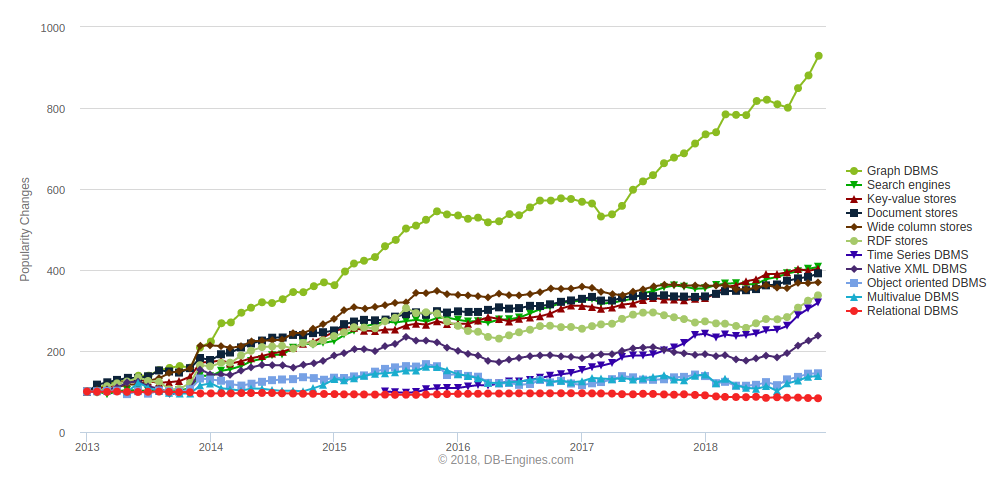
\includegraphics[width=150mm, keepaspectratio]{figures/graphdbms_trends.png}
	\caption{Adatbázisokban alkalmazott adatmodellek népszerűségének változása a \url{https://db-engines.com} oldal rangsorolása alapján}
	\label{fig:graphdbms_trends}
\end{figure}

Mi lehet a gráfadatbázisok \figref{graphdbms_trends}~ábrán is látható sikerének oka? Ezek a rendszerek több előnnyel is rendelkeznek a megszokott relációs adatbázisokhoz képest:

\begin{itemize}	
	\item \textbf{Intuitív adatmodell}: Az emberek szeretik úgy modellezni a világot, mint különböző entitások (csúcsok) és közöttük lévő kapcsolatok (élek) sokasága. Mind az entitások, mind a közöttük lévő kapcsolatok rendelkezhetnek különböző tulajdonságokkal, amelyek a tulajdonsággráfokkal egyszerűen kifejezhetőek.
	\item \textbf{Olvashatóság}: Ha megnézünk egy relációs adatbázison futtatott SQL  lekérdezést a séma ismerete nélkül, akkor nem magától értetődő, hogy egy attribútum egy tulajdonságot vagy kapcsolatot (idegen kulcs) jelent. A több-több kapcsolatoknál a kapcsolótáblák ezt egyértelműen meghatározzák, azonban a lekérdezés kevésbé olvasható lesz tőlük.
	\item \textbf{Tömörség}: Adott éltípusok mentén történő útkereső lekérdezéseket kifejezetten nehéz leírni SQL-ben és nem is minden SQL-dialektusban támogatottak. Még nehezebb a legrövidebb utat kereső lekérdezések megfogalmazása.
	\item \textbf{Gyors prototipizálás}: A gráfadatbázisok gyenge sémájának köszönhetően egyszerűbben létrehozhatók a prototípusok mint a relációs adatbázisoknál. Természetesen ennek következtében a lekérdezések optimalizálása bonyolultabbá válik a relációs lekérdezésekhez képest~\cite{DBLP:conf/cikm/SakrEH12}. Az egyik legnagyobb nehézséget a kapcsolatok kardinalitásának megbecslése jelenti körkörös illesztéseket tartalmazó lekérdezések esetében, melyre egy éltípuson történő ismételt navigálás megvalósításához van szükség. 
%	\item \textbf{Vizualizálás}: Egy gráfadatbázis, vagy annak részlete a megfelelő eszközök segítségével vizualizálva mélyebb betekintést adhat a teljes gráf struktúrájára vonatkozóan. Természetesen a megfelelő eszközök ritkák: a yWorks\footnote{\url{https://www.yworks.com/}} nevű cég yEd alkalmazása, vagy a Neo4j Bloom\footnote{\url{https://neo4j.com/bloom/}} alkalmazása nagyszerű, de használatuk nem ingyenes. A szabad szoftverek közül számos esetben egyedül a Graphviz\footnote{\url{https://www.graphviz.org/}} tud jó megjelenítést nyújtani.
\end{itemize}

A fentieket figyelembe véve elmondható, hogy sok esetben érthetőbb adathalmazt, valamint tömörebb lekérdezéseket eredményez a gráfadatbázisok használata. Azonban mivel ezek a rendszerek az informatika és a számítástudomány világában annyira újnak számítanak, hogy számos nyitott kérdés van velük kapcsolatban. Az egyik ilyen kérdés a gráfalapú lekérdezések és lekérdezőnyelvekkel kapcsolatos. Mivel a relációs adatbázisokban a -- legtöbbször SQL-ben megfogalmazott -- lekérdezések optimalizációjára igen hatékony megoldások léteznek, ezek bizonyos esetekben nem működnek jól a gráfadatbázisokban. Ezeknek az eseteknek az azonosítása az egyik legnagyobb nyitott kérdés. További fontos kérdés, hogy az ezeket a problémákat megoldó, illetve a már meglévő megoldások -- pl. a relációs adatbázisokban megszokott kétoperandusú illesztés (join) műveletek -- mennyire hatékonyak. Az alapvető problémák azonosításán és megoldásán túl fontos kérdés, hogy egyéb, a relációs adatbázisokban elterjed módszerek (pl. inkrementális nézetkarbantartás) hogyan ültethetőek át a gráfadatbázisokba.

Dolgozatomban megvizsgáltam, hogy mennyire hatékonyak a klasszikus relációs, és a modern gráfadatbázis-kezelők a gráfjellegű lekérdezések számítására.
Az ehhez szükséges elméleti háttér (\ref{sec:hatterismeretek}.~fejezet) megismerése után a kiértékeléshez kiválasztottam egy széleskörben elfogadott, sok nyelvi elemet és teljesítmény-aspektust lefedő teljesítménymérési keretrendszert, az LDBC Social Network Benchmarkot. A benchmark keretrendszerében javítottam a specifikáció hiányosságait és hibáit, ezek alapján frissítettem a benne található lekérdezéseket és szoftvermodulokat (\ref{sec:keretrendszer}.~fejezet).
A klasszikus adatbázis-kezelőkön kívül megvizsgáltam a differenciális adatfolyamot, mint alacsony válaszidővel rendelkező, elosztott, iteratív és inkrementális számításokat együttesen támogató számítási modellt. Az inkrementális lekérdezésekben nyújtott teljesítményének és a megközelítés használhatóságának tanulmányozásához a Transformation Tool Contest gráftranszformációs verseny (\ref{sec:ttc}.~fejezet) egyik feladatát valósítottam meg.
Az így rendelkezésre álló implementációk segítségével elkészítettem a különböző adatmodellt, nyelvet és megközelítést alkalmazó rendszerek összehasonlító teljesítménymérését (\ref{sec:kiertekeles}.~fejezet).
Végezetül áttekintettem a kapcsolódó kutatási eredményeket (\ref{sec:kapcsolodo}.~fejezet), amelyek alapján javaslatot tettem a tanszéken fejlesztett \emph{ingraph} rendszer továbbfejlesztésére. Végezetül pedig meghatároztam a további kutatási irányokat (\ref{sec:osszefoglalo}.~fejezet).

% !TeX spellcheck = hu_HU
% !TeX encoding = UTF-8
\chapter{Háttérismeretek}\label{sec:hatterismeretek}
\section{Esettanulmány}
Az ebben a fejezetben bemutatásra kerülő különböző adatmodellek és lekérdezőnyelvek összehasonlítása egy közös, gráf alapú adathalmazon fog történni, így először ezt mutatom be. A példa egy közösségi háló lehetséges adatbázisának egy részlete. \Aref{fig:example-graph}.~ábrán látható a példa gráfos ábrázolása, melyről leolvashatóak az alábbi adatok:
\begin{itemize}
	\item \textbf{Bob}: \uline{53 éves}, \uline{angolul} és \uline{németül} beszél.
	\item \textbf{Alice}: \uline{24 éves}, \uline{angolul} beszél, \textit{érdeklődik} a \textbf{Neofolk} iránt. \textbf{Alice} \textit{ismeri} \textbf{Bob}ot.
	\item A \textbf{Neofolk} \textit{egy} \textbf{Népzene}i műfaj.
	\item A \textbf{Népzene} \textit{része} a \textbf{Zené}nek, amely \textit{része} a \textbf{Művészet}nek.
\end{itemize}
A példa tehát \textbf{csúcsok}ból (csomópontokból), azok \uline{tulajdonság}aiból és a csúcsok között lévő kapcsolatokból, azaz \textit{élek}ből áll.
\begin{figure}[h]
	\centering
	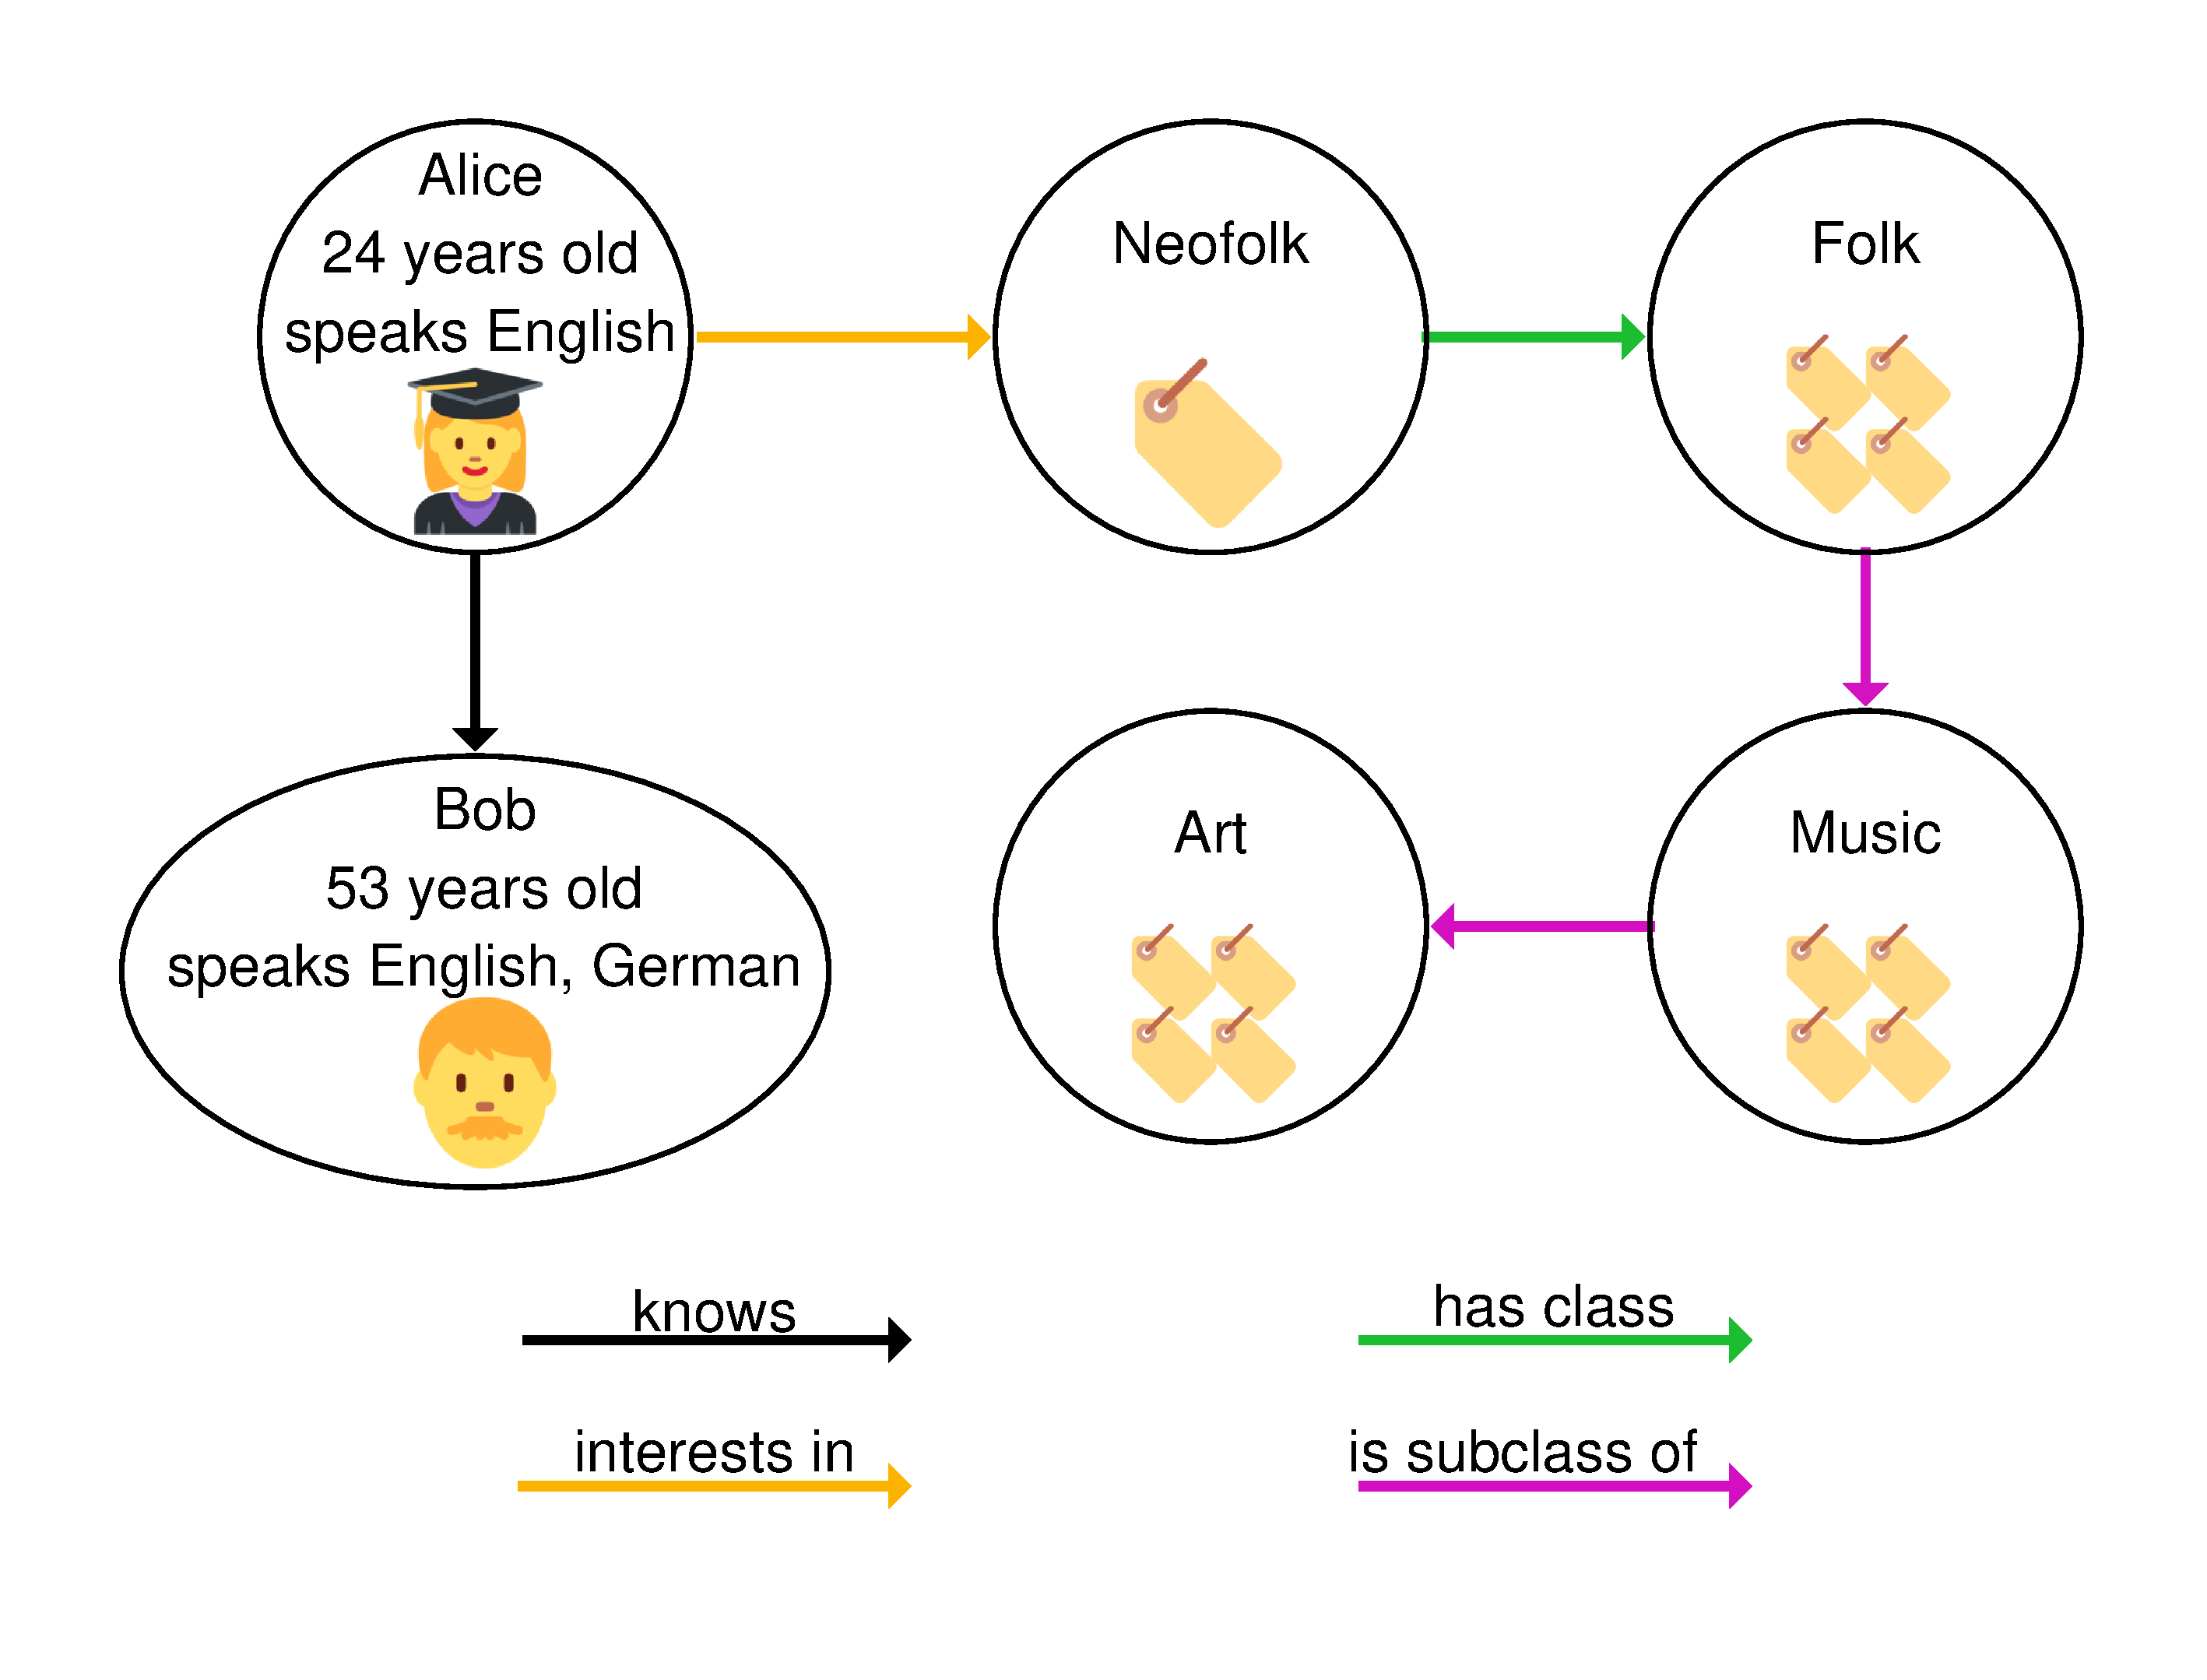
\includegraphics[scale=0.24]{example-graph.pdf}
	\caption{A példa gráf}
	\label{fig:example-graph}
\end{figure}
\section{Adatmodellek}
Az adatmodellek a példában megismert alkotórészek (csúcsok, élek és tulajdonságok) lehetséges használatának, jellemzőinek szempontjából igen különbözőek. Ezeket a különbségeket mutatja be \aref{tab:datamodels}.~táblázat. Jól látható, hogy a spektrum egyik vége a matematikában is megszokott irányított gráfok, a másik vége pedig az egyik legújabb adatmodell, a tulajdonsággráf. Az irányított gráfokkal ellentétben a címkézett gráfok csúcsainak már lehetnek típusai, amelyeket a megfelelő címkék csúcshoz rendelésével lehet meghatározni. Ha egy gráf csúcsain kívül az éleit is címkékkel látjuk el, akkor szemantikus gráfot kapunk. A tulajdonsággráf esetében a gráf csúcsainak és éleinek nem csak típusuk, hanem tulajdonságaik is lehetnek. Egy tulajdonság az egyszerű numerikus vagy szöveges adattípusokon túl akár komplexebb típus is lehet, például lista vagy halmaz.

A táblázatban továbbá látható az objektum-orientált modell, amely nem egyértelmű, hogyan kapcsolódik a gráf alapú adatmodellekhez: ha egy címkézett gráf csúcsainak lehetnek tulajdonságai, akkor az megfeleltethető a széles körben használt objektum-orientált modellnek. Fontos megjegyezni, hogy elméletben az objektum-orientált modellben is lehet az éleknek tulajdonsága, de ezt a gyakorlati megvalósítások közül elhanyagolható számú támogatja csupán. A továbbiakban három adatmodell kerül részletes bemutatásra a táblázatból: a szemantikus gráfok, a tulajdonsággráfok és a relációs adatmodell.
\begin{table}[h]
	\centering
	\begin{tabular}{@{\extracolsep{4pt}}lcccc@{}}
		\toprule
		\multicolumn{1}{c}{\multirow{3}{*}{adatmodell}} & \multicolumn{4}{c}{adatmodell tulajdonság} \\
		\cline{2-5}
		 & \multicolumn{2}{c}{csúcsok} & \multicolumn{2}{c}{élek} \\
		 \cline{2-3} \cline{4-5}
		 & típus & tulajdonság & típus & tulajdonság \\
		\midrule
		irányított gráf & $\circ$ & $\circ$ & $\circ$ & $\circ$ \\
		címkézett gráf & $\bullet$ & $\circ$ & $\circ$ & $\circ$ \\
		szemantikus gráf & $\bullet$ & $*$ & $\bullet$ & $\circ$ \\
		objektum-orientált modell & $\bullet$ & $\bullet$ & $\bullet$ & $\circ$ \\
		tulajdonsággráf & $\bullet$ & $\bullet$ & $\bullet$ & $\bullet$ \\
		\bottomrule
	\end{tabular}
	\caption{Az adatmodellek tulajdonságainak összehasonlítása}
	\label{tab:datamodels}
\end{table}
\subsection{Tulajdonsággráf}
A \emph{tulajdonsággráf} (property graph, PG) egy $G = (V, E, \verticestoedges, \vertexlabels, \edgelabels, \vertexlabelfunction, \edgelabelfunction, \vertexproperties, \edgeproperties)$ struktúrával írható le, ahol $V$ a csúcsok (csomópontok) halmaza, $E$ az élek halmaza és $\verticestoedges: E \assign V \cartesianproductop V$ függvény határozza meg az élek kiindulási és cél csúcsát~\cite{DBLP:conf/adbis/MartonSV17}. Formálisan a csúcsok típusát címkének nevezzük, az élek esetében pedig formálisan is típusról beszélünk:
\begin{itemize}
	\item $\vertexlabels$ a címkék halmaza, a $\vertexlabelfunction: V \assign 2^{\vertexlabels}$ függvény pedig \emph{a címkék egy halmazát} rendeli a csúcsokhoz.
	\item $\edgelabels$ a típusok halmaza, a $\edgelabelfunction: E \assign \edgelabels$ függvény pedig \emph{pontosan egy típust} rendel minden élhez.
\end{itemize}

A tulajdonságok definiálásához legyen $D = \bigcup_i D_i$ a különböző $D_i$ elemi domének uniója, és legyen $\relnull$ a \texttt{NULL} érték.
\begin{itemize}
	\item $\vertexproperties$ a csúcsok tulajdonságainak halmaza. A $p_i \in \vertexproperties$ csúcstulajdonság egy függvény $p_i: V \assign D_i \unionop \{ \relnull \}$, amely egy csúcstulajdonság értéket rendel a $D_i \in D$ doménből a $v \in V$ csúcshoz, ha $v$ rendelkezik a $p_i$ csúcstulajdonsággal, egyébként $p_i(v)$ értéke $\relnull$.
	\item $\edgeproperties$ az élek tulajdonságainak halmaza.A $p_j \in \edgeproperties$ éltulajdonság egy függvény $p_j: E \assign D_j \unionop \{ \relnull \}$, amely egy éltulajdonságot rendel a $D_j \in D$ doménből az $e \in E$ élhez, ha $e$ rendelkezik a $p_j$ éltulajdonsággal, egyébként $p_j(e)$ értéke $\relnull$.
\end{itemize}
A továbbiakban a csúcs- és éltulajdonságokat is tulajdonságnak hívjuk, csak ott különböztetjük meg őket ahol a megértés könnyebbsége miatt szükséges. 

Legyen $r$ reláció n-esek egy \emph{multihalmaza} (bag). Ekkor $r$ egy gráf reláció a $G$ tulajdonsággráfon, ha igaz az alábbi:

$$\forall A \in \schema{r}: \dom{A} \subseteq V \union E \union D,$$

ahol $sch(r)$ jelöli $r$ sémáját, azaz $r$-ben lévő attribútumok neveinek listáját, $dom(A)$ az $A$ attribútum doménjét, továbbá $V$ és $E$ a definíció szerint a gráf csúcsait és éleit jelölik. 

\Aref{fig:example-pg}.~ábrán látható a példa gráf tulajdonsággráf vizuális modellje, a tulajdonsággráf formális modellje pedig az alábbi:

\begin{align*}
	\vertexlabels &= \{\atom{Person}, \atom{Student}, \atom{Class}, \ldots \}\\
	\edgelabels &= \{\atom{KNOWS}, \atom{INTEREST}, \atom{CLASS}, \atom{SUBCLASS\_OF}\}\\
	\vertexproperties &= \{\atom{name}, \atom{speaks}, \atom{age}, \ldots\}\\
	\edgeproperties &= \{\atom{since}\}\\
	V &= \{a, b, c, d, e, f\}\\E &= \{1, 2, 3, 4, 5\}\\
	\verticestoedges&:\ 1 \assign \tuple{a, c}, 2 \assign \tuple{b, c}, \ldots\\
	\vertexlabelfunction&:\ b \assign \{\atom{Person}\}, a \assign \{\atom{Person}, \atom{Student}\}, \ldots\\
	\edgelabelfunction&:\ 1 \assign \atom{KNOWS}, 3 \assign \atom{CLASS}, \ldots\\
	\atom{name}&:\ a \assign \atom{``Alice"}, b \assign \atom{``Bob"}, e \assign \relnull, \ldots\\
	\atom{since}&:\ 1 \assign \atom{2014}, 2 \assign \relnull, 3 \assign \relnull, \ldots \\
	\ldots
%	\atom{age}&:\ \ldots\\
%	\atom{speaks}&:\ \ldots\\
%	\atom{topic}&:\ \ldots\\
%	\atom{level}&:\ \ldots\\
%	\atom{subject}&:\ \ldots
\end{align*}
\begin{figure}
	\centering
	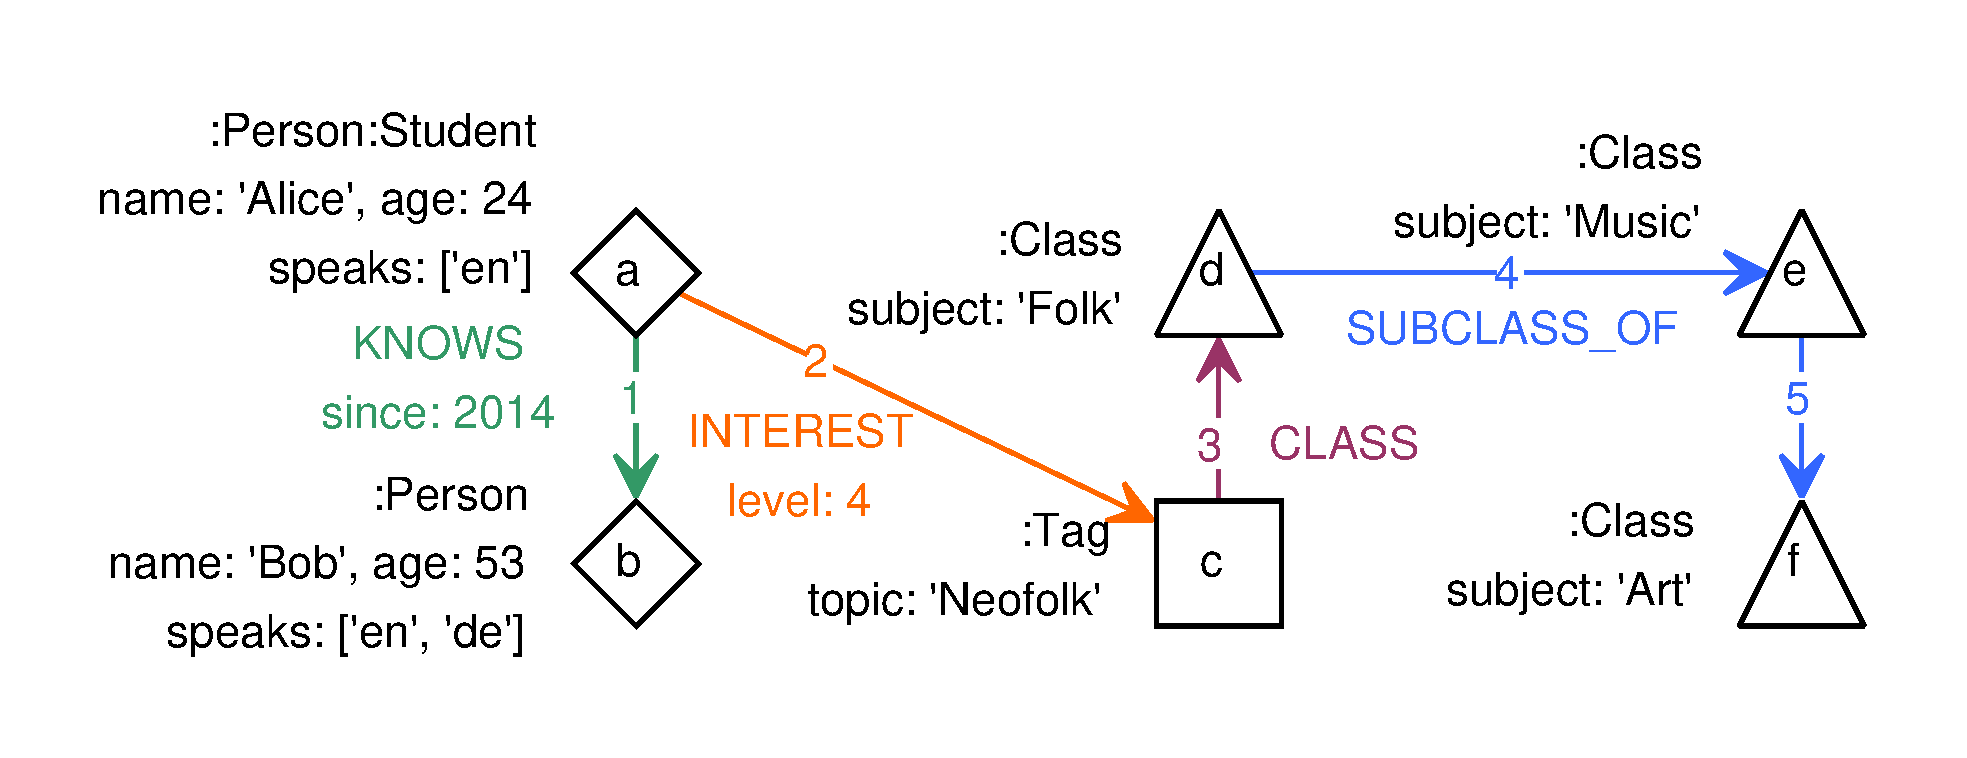
\includegraphics[scale=0.32]{example-pg.pdf}
	\caption{A példa tulajdonsággráf modellje. $\Diamond$~Person, $\Box$~Tag, $\triangle$~TagClass}
	\label{fig:example-pg}
\end{figure}
\subsection{Szemantikus gráf}

A szemantikus gráf olyan speciális adatmodell, amelyben egy gráfban találhatóak a metamodell és a példánymodell elemei. A szemantikus gráfnak számos reprezentációja létezik, ezek közül az egyik leggyakoribb a World Wide Web Consortium (W3C)\footnote{\url{https://www.w3.org/}} gondozásában lévő Resource Description Framework (RDF)\footnote{\url{https://www.w3.org/standards/techs/rdf}}. Mivel az RDF pontos definíciója meghaladja e dolgozat kereteit, ezért csak a legfontosabb részeket emeltem ki a specifikációból.

Egy RDF gráf hármasok egy halmaza. Egy hármas elemei az alábbiak:
\begin{itemize}
	\item alany, amely egy IRI hivatkozás vagy egy üres csomópont
	\item állítmány, amely egy IRI hivatkozás
	\item tárgy, amely egy IRI hivatkozás, egy literál vagy üres csomópont
\end{itemize}
Az IRI\footnote{Formális definíció:\url{ https://www.w3.org/TR/2014/REC-rdf11-concepts-20140225/\#section-IRIs}} (Internationalized Resource Identifier) egy UNICODE karakterlánc, amely egyértelműen azonosítja a gráf elemeit. Egy RDF gráfban az üres csomópontokat egy végtelen halmazból nyerjük. Az üres csomópontoknak ez a halmaza, továbbá az összes IRI hivatkozás halmaza, valamint az összes literál halmaza páronként diszjunkt halmazokat alkotnak. Formálisan tehát legyen $I$ az IRI-k halmaza, $B$ az üres csomópontok halmaza, $L$ pedig a literálok halmaza, akkor az $(s,p,o) \in (I \union B) \times I \times (I \union B \union L)$ egy RDF hármas, ahol $s$ az alany, $p$ az állítmány és $o$ a tárgy. A példa egy részletének megfelelő RDF szöveges reprezentációja\footnote{N-Triples formátumról bővebben: \url{https://www.w3.org/TR/n-triples/}}:
\begin{lstlisting}[frame=single]
a type Person .
a type Student .
a name "Alice" .
a age 24 .
a knows _:tmp1 .
_:tmp1 hasPerson b .
b name "Bob" .
\end{lstlisting}
Ebben példában az IRI-k halmaza $\{a, b, Person, Student, type, name, age, knows, hasPerson\}$, a literálok halmaza $\{``Alice", ``Bob", 24\}$ és az üres csomópontok halmaza pedig $\{_:tmp1\}$.

\begin{figure}[h]
	\centering
	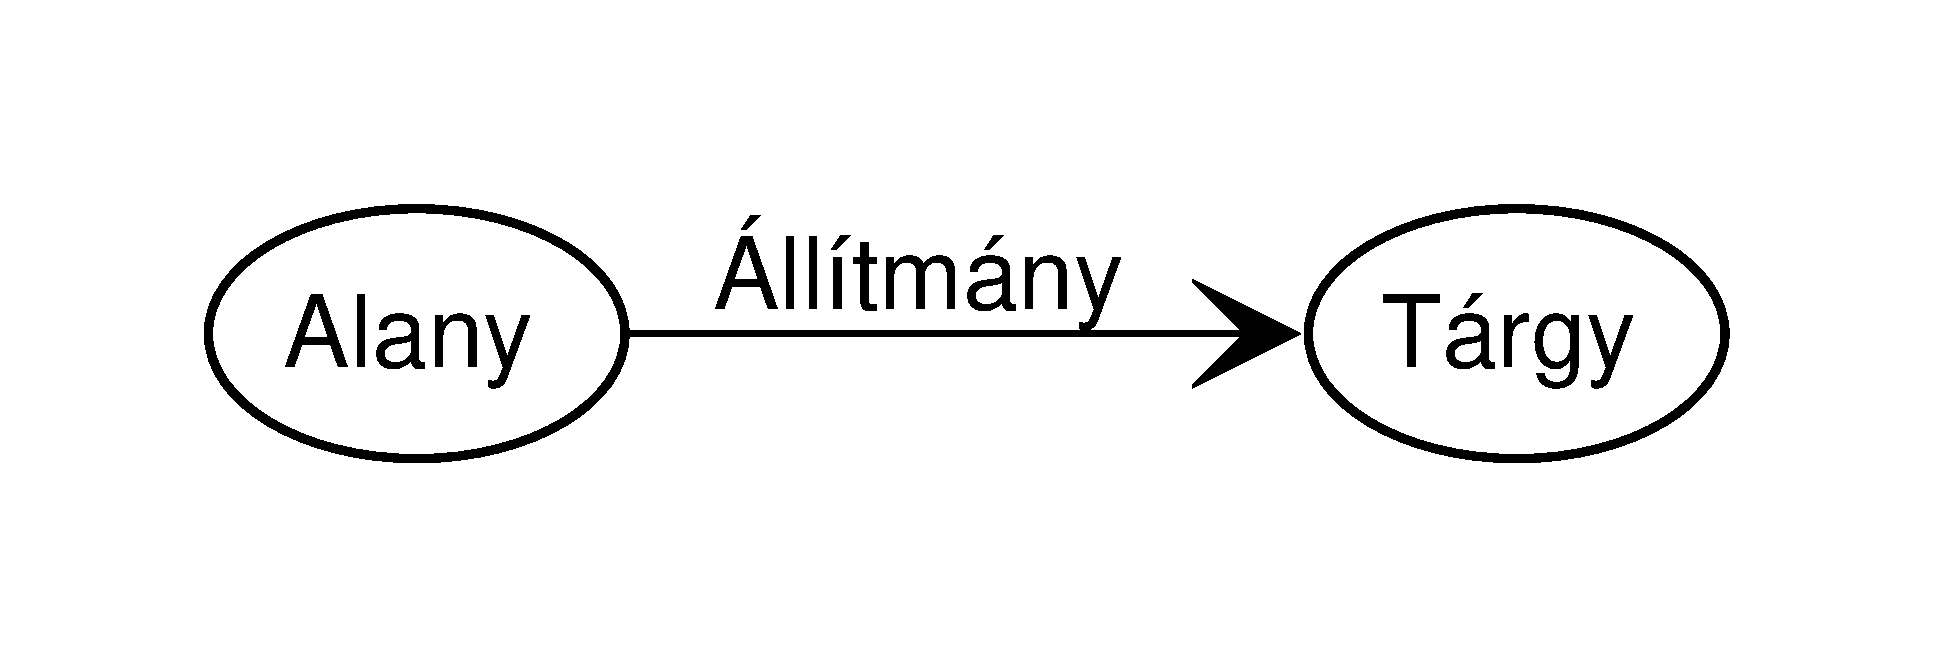
\includegraphics[scale=0.2]{triple.pdf}
	\caption{Egy RDF hármas grafikus ábrázolása}
	\label{fig:triple}
\end{figure}

\begin{figure}
\centering
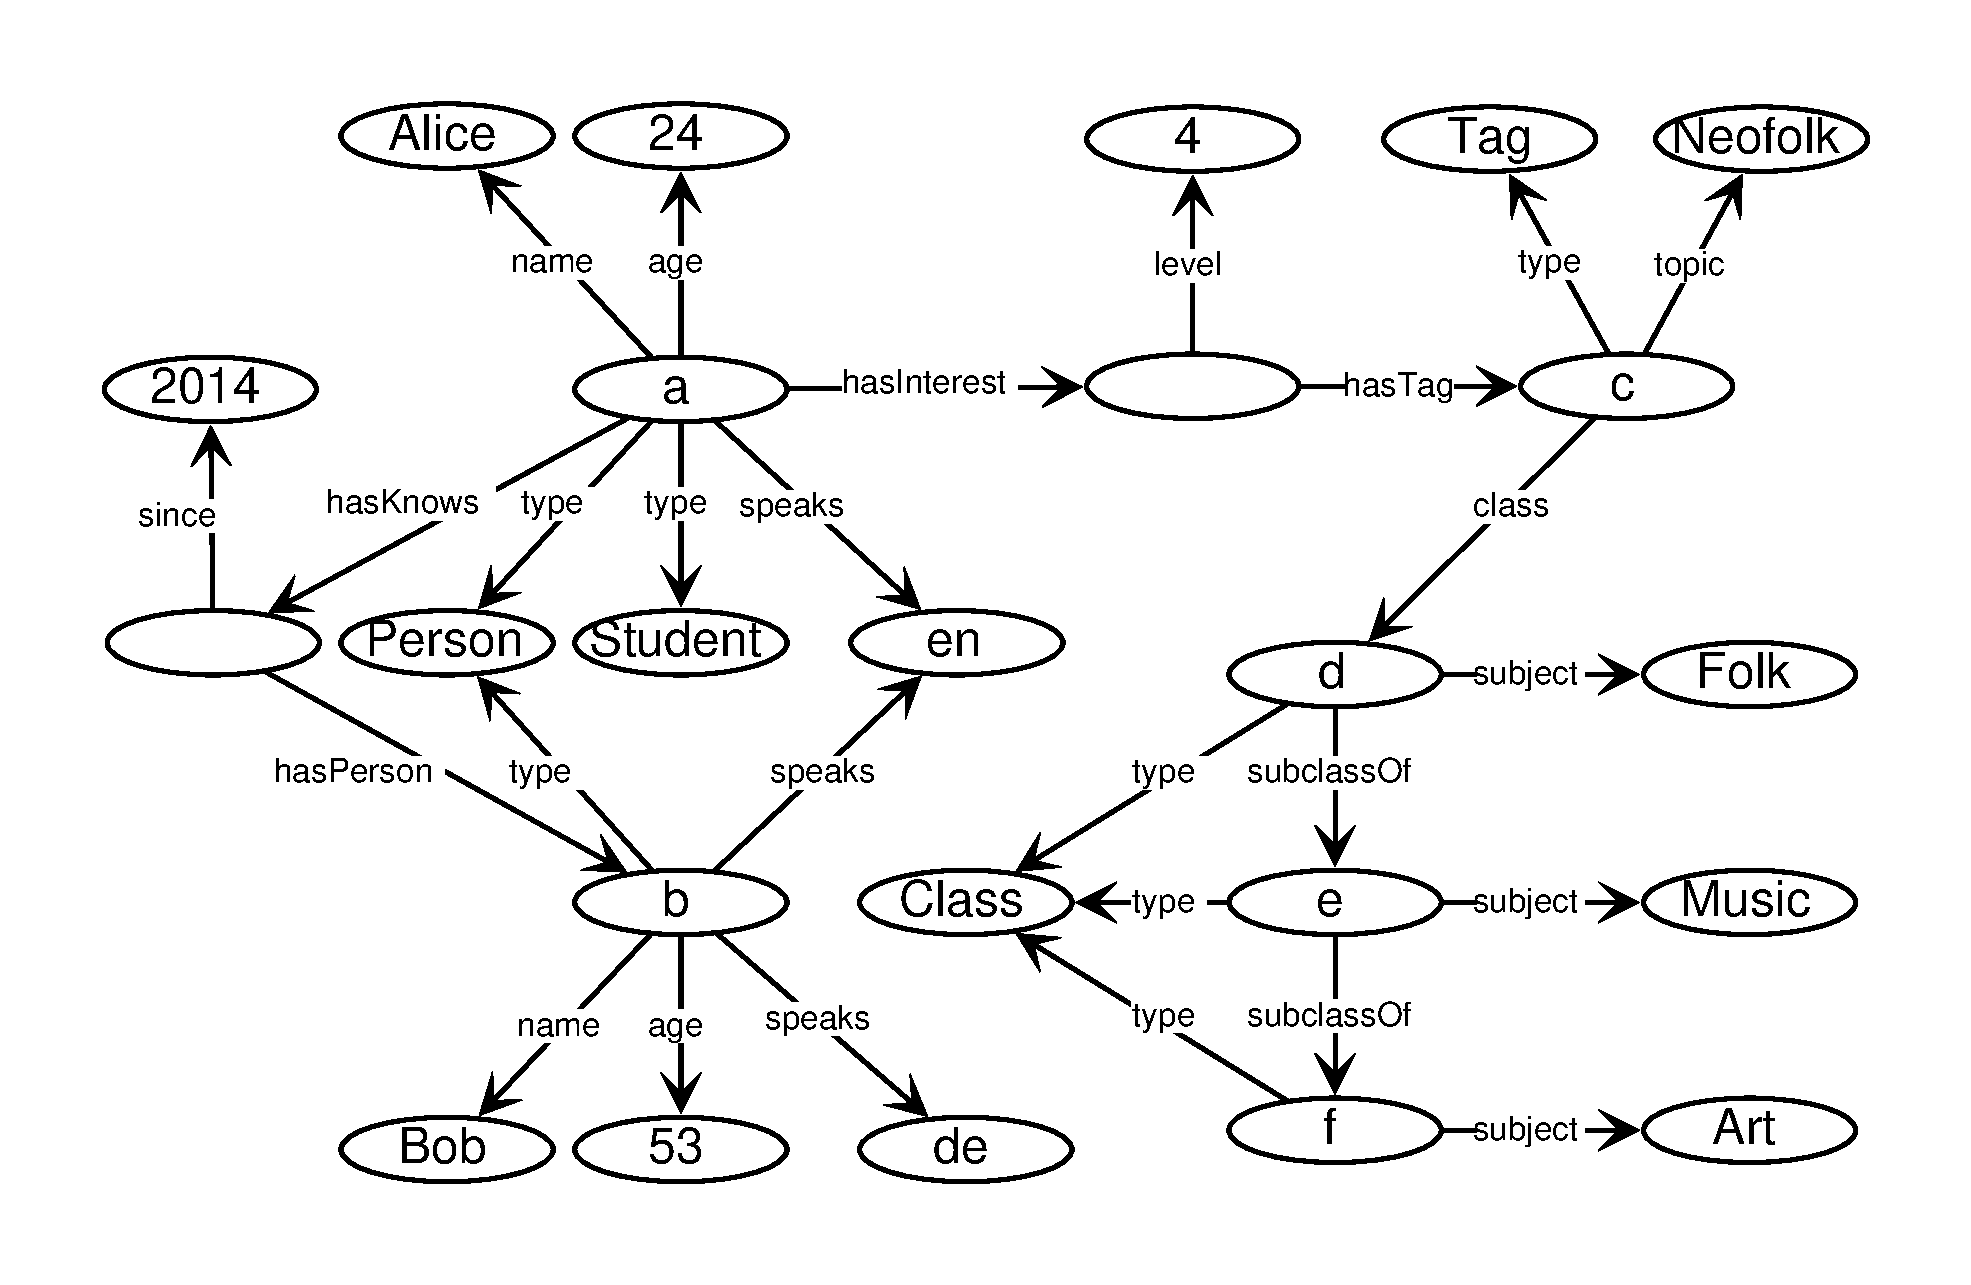
\includegraphics[scale=0.45]{example-rdf.pdf}
\caption{A példa RDF gráf modellje}
\label{fig:example-rdf}
\end{figure}

Az RDF gráf csomópontjainak halmazát a gráf hármasainak alanyai és tárgyai alkotják, az élek halmazát pedig a gráf hármasainak állítmányai alkotják. Egy hármas grafikusan ábrázolható két csomóponttal és a közöttük lévő irányított éllel, ahogy \aref{fig:triple}.~ábrán látható. Ilyen módon megkaphatjuk a példa RDF gráf modelljének \aref{fig:example-rdf}.~ábrán látható grafikus vizualizációját. Az ábrán látható, hogy az RDF gráfok csúcs- és élcímkézett irányított gráfok.

\Aref{tab:datamodels} táblázat szemantikus gráfhoz tartozó sorában látható $*$ azt jelenti, hogy bár egy RDF gráfban a csúcsoknak nem lehet tulajdonsága, de a csúcsok tulajdonságait egyszerűen leképezhetjük hármasokká, ahogy a példa gráf RDF gráfján látszik: az eredeti gráf \textit{name} tulajdonságát az RDF gráfban az azonos nevű állítmánnyal rendelkező hármas jelenti.

\subsection{Relációs adatmodell}
\label{sec:relacios-adatmodell}

A dolgozatban megemlített adatmodellek közül a relációs adatmodell a legrégebb óta használt és kutatott modell. Ebben a fejezetben az E. F. Codd által leírt definíciót~\cite{DBLP:journals/cacm/Codd70} ismertetem.
Adottak \set{1}, \set{2}, \dots, \set{n} nem feltétlenül különböző halmazok, ekkor \rel{} egy reláció ezen az $n$ halmazon, ha \rel{} $\subseteq{}$ \set{1} $\times$ \set{2} $\times$ \dots $\times$ \set{n}. Ilyenkor az \set{i} halmaz az \rel{} $i.$ doménje.

Gyakran a relációkat táblázatokként ábrázoljuk. Az \rel{} relációt ábrázoló táblázat minden sora megfeleltethető pontosan egy elemnek \rel{}-ből, így a reláció elemeit a reláció sorainak is nevezzük.
Az oszlopok sorrendje követi az \set{1}, \set{2}, \dots, \set{n} sorrendet, azaz az $i.$ oszlop az $i.$ domén értékeit tartalmazza. Az oszlopokat szokás a hozzájuk tartozó domén nevével felcímkézni, ezzel egyértelműsíteni a jelentésüket. Esetenként az oszlopokra egyszerűen a nevükkel hivatkozunk és nem vesszük figyelembe az attribútumok sorrendjét.

A relációk lehetnek \emph{halmaz} (set) szemantikájúak, ebben az esetben az elemeik egyediek, valamint \emph{multihalmaz} szemantikájúak, amikor az elemeiek között előfordulhatnak ismétlődések. A reláció elemeinek sorrendje egyik esetben sem számít.

A példa relációs modellje \aref{fig:example-rdf}.~ábrán látható. Megfigyelhető, hogy a példában minden csúcstípushoz (\textsf{Persons}, \textsf{Tags}, \textsf{TagClasses} relációk), minden többes kardinalitású csúcs tulajdonságához (\textsf{Speaks}) és minden éltípushoz (\textsf{Interests}, \textsf{SubclassOf}, \textsf{HasClass}) külön reláció tartozik: ez gyakori leképzése a gráfoknak a relációs adatmodellre. További fontos megfigyelés, hogy az éleket jelentő relációknak (\textsf{Knows}, \textsf{Interests}, \textsf{SubclassOf}, \textsf{HasClass}) nincsen azonosítója, mert ezeket az él kezdő- és végpontja azonosítja. Ez a séma feltételezi, hogy két csúcs között nem vezet egynél több azonos él (ugyanolyan típusú él vezethet, ha legalább egy éltulajdonságban eltérnek), továbbá hogy tanulók csak személyek lehetnek (\textsf{Students} reláció).

\begin{figure}[htb]
	\begin{subfigure}[b]{0.22\textwidth}
		\begin{center}
			\begin{tabular}{|c|l|c|}
				%\hline
				%\multicolumn{3}{|c|}{\bf persons} \\
				\hline
				id & \multicolumn{1}{|c|}{name} & age \\
				\hline
				a & Alice & 24 \\
				\hline
				b & Bob & 53 \\
				\hline \\
			\end{tabular}
			\caption{\textsf{Persons}}
			\label{example-rdb-persons}
		\end{center}
	\end{subfigure}
	\begin{subfigure}[b]{0.16\textwidth}
	\begin{center}
		\begin{tabular}{|c|c|c|}
			%\hline
			%\multicolumn{3}{|c|}{\bf interests} \\
			\hline
			personId \\
			\hline
			a \\
			\hline \\ \\
		\end{tabular}
		\caption{\textsf{Students}}
		\label{example-rdb-students}
	\end{center}
	\end{subfigure}
	\begin{subfigure}[b]{0.2\textwidth}
		\begin{center}
			\begin{tabular}{|c|l|}
				%\hline
				%\multicolumn{2}{|c|}{\bf tags} \\
				\hline
				id & \multicolumn{1}{|c|}{topic} \\
				\hline
				c & Neofolk \\
				\hline \\ \\
			\end{tabular}
			\caption{\textsf{Tags}}
			\label{example-rdb-tags}
		\end{center}
	\end{subfigure}
	\begin{subfigure}[b]{0.2\textwidth}
		\begin{center}
			\begin{tabular}{|c|l|}
				%\hline
				%\multicolumn{2}{|c|}{\bf tagClasses} \\
				\hline
				id & \multicolumn{1}{|c|}{subject} \\
				\hline
				d & Folk \\
				\hline
				e & Music \\
				\hline
				f & Art \\
				\hline
			\end{tabular}
			\caption{\textsf{TagClasses}}
			\label{example-rdb-tagclasses}
		\end{center}
	\end{subfigure}
	\begin{subfigure}[b]{0.16\textwidth}
		\begin{center}
			\begin{tabular}{|c|c|}
				%\hline
				%\multicolumn{2}{|c|}{\bf hasClass} \\
				\hline
				tag & class\\
				\hline
				c & d \\
				\hline \\ \\
			\end{tabular}
			\caption{\textsf{HasClass}}
			\label{example-rdb-hasClass}
		\end{center}
	\end{subfigure}

	\

	\begin{subfigure}[b]{0.2\textwidth}
		\begin{center}
			\begin{tabular}{|c|c|}
				%\hline
				%\multicolumn{2}{|c|}{\bf subclassOf} \\
				\hline
				src & trg\\
				\hline
				d & e \\
				\hline
				e & f \\
				\hline \\
			\end{tabular}
			\caption{\textsf{SubclassOf}}
			\label{example-rdb-subclassOf}
		\end{center}
	\end{subfigure}
	\begin{subfigure}[b]{0.26\textwidth}
		\begin{center}
			\begin{tabular}{|c|c|c|}
				%\hline
				%\multicolumn{3}{|c|}{\bf knows} \\
				\hline
				src & trg & since\\
				\hline
				a & b & 2014 \\
				\hline \\ \\
			\end{tabular}
			\caption{\textsf{Knows}}
			\label{example-rdb-knows}
		\end{center}
	\end{subfigure}
	\begin{subfigure}[b]{0.28\textwidth}
		\begin{center}
			\begin{tabular}{|c|c|c|}
				%\hline
				%\multicolumn{3}{|c|}{\bf interests} \\
				\hline
				person & tag & level\\
				\hline
				a & d & 4 \\
				\hline \\ \\
			\end{tabular}
			\caption{\textsf{Interests}}
			\label{example-rdb-interests}
		\end{center}
	\end{subfigure}
	\begin{subfigure}[b]{0.24\textwidth}
	\begin{center}
		\begin{tabular}{|c|c|}
			%\hline
			%\multicolumn{2}{|c|}{\bf speaks} \\
			\hline
			personId & lang\\
			\hline
			a & en \\
			\hline
			b & de \\
			\hline
			b & en \\
			\hline
		\end{tabular}
		\caption{\textsf{Speaks}}
		\label{example-rdb-speaks}
	\end{center}
	\end{subfigure}

	\caption{A példa relációs modellje}
	\label{fig:example-rdb}
\end{figure}

\section{Lekérdezőnyelvek}
Az utóbbi évtizedben a gráf alapú adatbázisok elterjedtek mind az ipari, mind az akadémiai területeken. Az adatbázisok ezen új generációja által nyújtott új szolgáltatások (gráfminták megfogalmazása, gráf algoritmusok használata, részgráf illesztész) használatához szükségessé vált új lekérdezőnyelvek megalkotása. Ebben a fejezetben bemutatok három új lekérdezőnyelvet és természetesen a relációs adatbázisok (relational databases, RDB) lekérdezőnyelvét, az SQL-t is bemutatom. A lekérdezőnyelvek bemutatása során a dolgozat megértéséhez szükséges részletekre fókuszálok, mivel a nyelvek részletes bemutatása meghaladja a dolgozat kereteit. A bemutatott nyelveken egy egyszerű lekérdezést is megfogalmazok a nyelvek szemléltetése miatt: ``adjuk vissza az emberek nevét és ismerőseik számát!''




\subsection{Relációalgebra}
\label{sec:relacioalgebra}

Az adatbázis-kezelés egyik legismertebb formális nyelve a relációalgebra, mely a relációs adatmodell (\ref{sec:relacios-adatmodell}. szakasz) feletti különböző halmazműveleteket definiál~\cite{gajdos,DBLP:books/daglib/0020812,DBLP:books/daglib/0015084}. Az alábbiakban röviden áttekintem a legtöbbet használt relációalgebrai operátorokat.

\subsubsection{Unáris operátorok}
A \emph{projekció} operátor $ \projection{A} \left(r\right)$ a bemeneti $r$ relációt olyan relációra alakítja, ami csak az $A$ halmazban szereplő attribútumokat tartalmazza. A projekció operátor képes továbbá attribútumok átnevezésére is az alábbi jelöléssel: $ \projection{x1 / y1, x2 / y2, \ldots} \left(r\right)$.
A \emph{szelekció} operátor $ \selection{\theta} \left(r\right) $ a bemeneti $r$ reláció azon sorait tartja meg, melyek kielégítik a $\theta$ logikai kifejezést.

\paragraph{Multihalmazok felett értelmezett műveletek}

A \emph{duplikátumszűrés} operátor ($\duplicateeliminationop$) a bemeneti relációból olyan relációt készít, amiben nincsenek azonos sorok. Más szavakkal a bemeneti multihalmaz szemantikájú relációt halmaz szemantikájúra alakítja.
A \emph{csoportosítás} operátor ($\groupingop$) a reláció sorait egy adott attribútumhalmaz szerint csoportosítja, majd a fennmaradó attribútumokat aggregálja. A $\grouping{e_1, e_2, \ldots }{c_1, c_2, \ldots } (r)$ kifejezés az $r$ reláció sorait a $c_1, c_2, \ldots $ kritériumattribútumok mentén csoportosítja, majd minden csoportra kiszámítja a $\tuple{e_1, e_2, \ldots }$ sorok értékét.


\subsubsection{Bináris operátorok}

\paragraph{Illesztés jellegű műveletek}

Az \emph{illesztés} (join) jellegű műveletek két reláció összekapcsolását végzik el, általában növelve az attribútumok számát. Az illesztés jellegű műveletek alapja a \emph{Descartes-szorzás} (Cartesian product). A $r \times s$ kifejezés egy $n$ sorból álló $r$ és egy $m$ sorból álló $s$ relációból egy $n \cdot m$ sorú relációt állít elő, mely tartalmazza $r$ és $s$ minden attribútumát, valamint azok sorait minden lehetséges kombinációban.

A \emph{természetes illesztés} ($\joinop$) művelet az azonos nevű attribútumok mentén kapcsolja össze a bemeneti relációkat. Formálisan:
$$r \join s = \pi_{R \union S} \left(\selection{r.A_1 = s.A_1\,\land\,\ldots\,\land\,r.A_n = s.A_n)} \left(r \times s\right) \right)$$

Az \emph{antijoin operátor} ($\antijoinop$) a bal oldali bemeneti reláció azon sorait tartja meg, amikhez nincs illeszkedő sor a jobb oldali bemeneti relációban. Formálisan:
$$r \antijoin s = r \minus \projection{R} \left(r \join s\right)$$

A \emph{bal oldali külső illesztés} operátor (\leftouterjointext, $\leftouterjoin$)~\cite{DBLP:books/daglib/0015084} előállítja a két bemeneti reláció természetes illesztését, majd hozzáfűzi ehhez a baloldali reláció azon elemeit, amik nem kerültek be az illesztésbe, $\relnull$ elemekkel a megfelelő szélességűre kiegészítve. Formálisan,
$r \leftouterjoin s \equiv (r \join s) \union \left( (r \antijoin s) \times \tuple{\relnull}_{(S \minus R)} \right)$, ahol a $\tuple{\relnull}_{k}$ jelentése egy $k$ szélességű, $\relnull$ elemekből álló sor.

\paragraph{Unió műveletek}

Az unió művelet ($\union$) két relációt fűz össze az attribútumok mentén. Formálisan $t \in r \union s \iff (t \in r) \lor (t \in s)$.
A multihalmazok felett definiált relációalgebra esetén gyakran megkülönböztetik az unió operátor két típusát: a \emph{halmaz unió} ($\union$) operátor duplikátumszűrést végez, míg a \emph{multihalmaz unió} operátor ($\uplus$) esetén lehetnek duplikátumok a kimenetben. A kétféle unió operátor közötti összefüggés a $r \union s = \duplicateelimination{(r \uplus s)}$ kifejezéssel írható le. A dolgozatban a továbbiakban az unió operátor alatt a multihalmaz unió operátort értjük.

\paragraph{Példa}

A példa lekérdezés relációalgebrában az alábbi módon fogalmazható meg:
$$
\grouping{\var{p}.\atom{name}, \texttt{count}(f)}{\var{p}.\atom{name}}
\big[
\projection{\var{p}, \var{p}.\atom{name}} (\mathsf{Persons})
\leftouterjoin
\big(
\projection{\var{p}, \var{f}} (\mathsf{Knows}) \join \projection{\var{f}} (\mathsf{Persons})
\big)
\big]
$$

\subsection{Cypher}\label{sec:cypher}
A Cypher nyelv~\cite{DBLP:conf/sigmod/FrancisGGLLMPRS18} az egyik legelterjedtebb a nyelv tulajdonsággráfok lekérdezésére és módosítására. A nyelv a Neo4j gráfadatbázis-kezelőben jelent meg először, majd később számos másik termékben (SAP HANA Graph~\cite{DBLP:conf/btw/RudolfPBL13}, Redis Graph\footnote{\url{https://oss.redislabs.com/redisgraph/}}) implementálták. A kereskedelmi termékek mellett több kutatási projektben (ingraph~\cite{DBLP:conf/sdl/MartonSB17}, Cytosm~\cite{DBLP:conf/grades/SteerALCVV17}) is használni kezdték a Cyphert. Az openCypher\footnote{\url{https://www.opencypher.org/}} projekt 2015-ös elindulásával létrejött egy olyan platform, amelynek célja a Cypher nyelv új nyelvi elemeinek kollaboratív kidolgozása a különböző Cyphert használó termékek és projektek fejlesztőinek bevonásával. A projekt célja az, hogy a Cypher váljon az ipari szabvánnyá a tulajdonsággráfok lekérdezésére és módosítására. Fontos megjegyezni, hogy a projekttel együtt létrejött az openCypher nyelv is, amely a Cypher nyelv egy valódi részhalmaza, azonban nem tartalmazza az összes Cypherben lévő nyelvi konstrukciót (pl. \texttt{shortestPath}, \texttt{reduce} stb.). A dolgozat további részében mindig felhívom a figyelmet a két nyelv közötti különbségekre, ha azok nélkülözhetetlenek a megértés szempontjából.

\paragraph{Linearitás}
Egy Cyper lekérdezés bemenete egy tulajdonsággráf, kimenete pedig egy táblázat, amely tartalmazza a gráfból kinyert információt. A lekérdezések struktúrája lineáris: az állítások egymás után következnek a lekérdezésben. Az állítások tekinthetőek függvényeknek, amelyek bemenete és kimenete is egy táblázat. Az állítások módosíthatják az oszlopok számát, sorokat szűrhetnek ki és adhatnak hozzá a táblázathoz. Egy lekérdezés tehát ilyen függvények sorozata. Fontos azonban, hogy az állítások sorrendje szigorúan deklaratív jellegű, azaz a konkrét implementációk felcserélhetik két állítás végrehajtását, ha az nem változtatja meg az eredményt. A deklaratív jellegnek köszönhetően nem kell az SQL \keyword{SELECT}-hez hasonlóan rögtön a lekérdezés elején leírni a projekciót, hanem elég a lekérdezés végén a \keyword{RETURN} kulcsszóval. Az egyes állításokban szintén lehetséges projekciót végezni a \keyword{with} kulcsszóval. A \keyword{with} ugyanazokat a projekciókat engedi meg, mint a \keyword{return}, ideértve az aggregációt. Továbbá, a \keyword{with} támogatja az egyes mezők értéke szerinti szűrést. A lineáris komponálhatóságon túl a Cypher támogatja az olyan beágyazott lekérdezéseket, mint például az \keyword{union} lekérdezések.

\paragraph{Mintaillesztés}
A Cypher központi eleme a gráfminták megfogalmazása. A gráfminták Cypherben \texttt{(a)-[r]->(b)} alakúak, ahol \texttt{a} és \texttt{b} a gráf két csúcsát, \texttt{r} pedig az őket összekötő él típusát jelenti. Van lehetőség egy éltípusból alkotott utak megfogalmazására is \texttt{(a)-[r*x..y]->(b)} formában, ahol \texttt{x} és \texttt{y} tetszőleges egész számok az \texttt{x <= y} feltétellel. Opcionálisan \texttt{x} és \texttt{y} is elhagyható. A \keyword{MATCH} kulcsszó az ilyen módon megfogalmazott gráfminta lehetséges értékeit adja eredményül.

A nyelv mélyebb ismerete nem szükséges a dolgozat megértéséhez, így a további részleteket (gráfok módosítása, többes attribútumok és listák kezelése) nem mutatom be. A példa lekérdezés Cypher nyelven az alábbi:

\vspace{1.5ex}

\noindent\begin{minipage}{\textwidth}
\begin{lstlisting}[frame=single,label=listing:cypher-example,caption=Cypher példakód]
MATCH (p:Person)
OPTIONAL MATCH (p)-[:KNOWS]->(f:Person)
RETURN p.name, count(f)
\end{lstlisting}
\end{minipage}

Ahogy látható, a \keyword{OPTIONAL MATCH} kulcsszó használható egy gráfminta opcionális illesztésére. Fontos részlet, hogy az SQL-lel szemben Cypherben nem kell \keyword{GROUP BY} kulcsszóval megadni a nem aggregált tulajdonságokat.

\subsection{Gremlin}
A Gremlin~\cite{DBLP:conf/dbpl/Rodriguez15} az Apache TinkerPop\footnote{\url{http://tinkerpop.apache.org/}} projekt által tervezett, fejlesztett és terjesztett gráfbejáró automata és nyelv. A Cypherrel ellentétben a Gremlin nem csak gráf minták illesztését tudja elvégezni, hanem iteratív lekérdezéseket is megfogalmazhatunk használatával. A Gremlin továbbá elősegíti, hogy a felhasználó:
\begin{itemize}
	\item a saját programozási nyelvébe beágyazza,
	\item kiterjessze domén specifikus kifejezésekkel,
	\item a kiterjeszthető, fordítási idejű újraírási szabályokkal optimalizálja
	\item és egy számítógép-klaszteren futassa
\end{itemize}
a Gremlin lekérdezéseket.

A gráfbejáró automata három részből áll: egy $G$ gráfból (adat), egy $\Psi$ bejárási szekvenciából (instrukciók) és bejárók egy $T$ halmazából (olvasási/írási referenciák). Az automata magas szintű működése: a bejárók $T$ halmaza mozog a $G$ gráfon a $\Psi$-ben megfogalmazott instrukciók szerint. A számítás akkor ér véget, amikor már vagy nem létezik bejáró $T$-ben, vagy az összes létező bejáró megállt, azaz nem végez több instrukciót $\Psi$-ből. Az első esetben az eredmény egy üres halmaz, utóbbi esetben pedig a bejárók által hivatkozott $G$-beli helyek multihalmaz uniója.

A Gremlin lekérdezőnyelv egy funkcionális programozási nyelv. Célja annak biztosítása, hogy a felhasználók az emberek számára érthető kifejezésekkel, egyszerűen definiálhassák a bejárási szekvenciát, azaz egyszerűen hozzájussanak a számukra fontos információhoz. A nyelv építő elemei a függvénykompozíciók és a functor típusú objektumok. Például az $a \circ b \circ c$ kifejezés leírható \lstinline{a().b().c()} alakban. A függvényparaméterekkel pedig a bejárások egymásba ágyazása is lehetséges, például az $a (b \circ c) \circ d$ kifejezés \lstinline{a(b().c()).d()} alakban írható le.

\paragraph{Példa}

A példa lekérdezés Gremlin nyelven:

\vspace{1.5ex}

\noindent\begin{minipage}{\textwidth}
\begin{lstlisting}[frame=single,language=Java,caption=Gremlin példakód]
g.V().hasLabel('person').as('person').property('name').as('pName')
    .select('person').optional(outE('KNOWS').inV()).count()
    .select('pName', 'count')
\end{lstlisting}
\end{minipage}

\subsection{SPARQL}
Az RDF 1998-as megjelenésével együtt megjelent az igény az RDF gráfok lekérdezését, módosítását lehetővé tevő nyelvekre. 2004-ben a W3C RDF Data Access Working Group szervezete kiadta a Simple Protocol and RDF Query Language első publikus tervezetét. Azóta a SPARQL~\cite{DBLP:journals/tods/PerezAG09} elterjedt és az RDF gráfok szabványos lekérdezőnyelvévé vált.

Mivel az RDF egy irányított címkézett gráf adatmodell, ezért a SPARQL esszenciális része a gráfminták megfogalmazása. A SPARQL-ben az RDF gráfoknál ismertetett $I$, $B$ és $L$ halmazokon kívül létezik egy, velük diszjunkt $V$ halmaz, amely a változók egy végtelen halmaza. Egy SPARQL lekérdezést tekinthetünk $H \longleftarrow M$ alakúnak, ahol $M$ a lekérdezés törzse, egy komplex RDF gráfminta változókkal, opcionális részekkel, metszetekkel, különbségekkel és a változókra vonatkozó kényszerekkel, $H$ pedig a lekérdezés feje, egy kifejezés, amely megmondja, hogy hogyan állítsuk össze a lekérdezés eredményét. $H$ különböző módosítókat tartalmazhat, például sorrendet, limitet definiálhat, de tartalmazhat klasszikus relációalgebrai kifejezéseket is. Egy SPARQL lekérdezés kimenete változatos formátumú lehet: igen/nem válasz, egy táblázat vagy egy új RDF gráf. Egy $Q$ lekérdezés kiértékelése a $D$ RDF gráfon két lépésben történik: $Q$ törzsét illesztjük $D$-re, hogy a törzsben lévő változók lekötéseinek egy halmazát kapjuk, amelyet a fej kiértékelésekor használjuk fel. A SPARQL gráfminta rekurzív definíciója az alábbi:
\begin{enumerate}
	\item Egy hármas a $(I \union B) \times I \times (I \union B \union L)$ halmazból gráfminta.
	\item Ha $P_1$ és $P_2$ gráfminták, akkor ($P_1$ . $P_2$), ($P_1$ \keyword{OPTIONAL} $P_2$) és ($P_1$ \keyword{UNION} $P_2$) is gráfminták.
	\item Ha $P$ egy gráfminta és $R$ egy SPARQL feltétel, akkor $P$ \keyword{FILTER} $R$ is gráfminta.
\end{enumerate}
A pont szimbólum a minták összefűzését jelenti, tehát $P_1$-nek és $P_2$-nek is illeszkednie kell. Az \keyword{OPTIONAL} kulcsszó esetén pedig a $P_1$-re illeszkedő részgráfokon lekötésre kerülnek $P_2$ változói, ha $P_2$ illeszkedik a részgráfra. Egyéb esetben $P_2$ változói kötetlen változók lesznek.

\paragraph{Példa}

A példa lekérdezés SPARQL nyelven az alábbi:

\vspace{1.5ex}

\noindent\begin{minipage}{\textwidth}
\begin{lstlisting}[frame=single, morekeywords={SELECT}, caption=SPARQL példakód]
SELECT
    ?personName,
    (COUNT(friend) AS ?friendCount)
WHERE
{
    ?person a Person .
    ?person foaf:name ?personName .
    OPTIONAL {
        ?person knows/hasPerson ?friend .
        ?friend a Person
    }
}
GROUP BY ?personName
\end{lstlisting}
\end{minipage}
A példán látható, hogy SPARQL-ben a változókat a \texttt{?} prefixszel jelöljük.

\subsection{SQL}
Az SQL-t 1979-ben, az Oracle V2 megjelenésekor kezdték el használni relációs adatbázisok lekérdezésére, módosítására. Azóta iparági szabvánnyá vált, a relációs adatbázisok túlnyomó részében elérhető. Először 1986-ban szabványosították, azóta többször frissítették a szabványt, utoljára 2016-ban. A megjelenése óta számos más nyelv alapjául szolgált. A népszerűsége ellenére azonban az egyik legjelentősebb hiányosságát még manapság sem sikerült megjavítani: az SQL szabvány természetes nyelven írt, ebből adódóan sok részletet nem tud kellő pontossággal specifikálni. Az SQL-t többször próbálták már formalizálni~\cite{DBLP:journals/pvldb/GuagliardoL17}, de általánosan elfogadott megoldást eddig nem sikerült alkotni a szabvány kiterjedtsége és a \texttt{NULL} értékek kezelésével járó kihívások miatt.

Közismert, hogy az SQL a sikerét nagyban a deklaratív jellegének köszönheti. Így nem kell pontosan tudnunk, hogyan kell hatékonyan előállítani a számunkra fontos információt, csupán elég megfogalmazni azt, hogy milyen információra van szükségünk. Az adatbázis-kezelő feladata, hogy a lekérdezést lefordítsa, optimalizálja és végrehajtsa.

Az SQL számos nyelvi elemet tartalmaz, köztük a következőket:
\begin{itemize}
	\item Klózok (\keyword{SELECT}, \keyword{WHERE}, \keyword{LIMIT}, \keyword{JOIN} stb.), amelyek kompozíciója alkotja a lekérdezéseket és állításokat.
	\item Kifejezések, amelyek eredménye lehet egy skalár vagy egy sorokból és oszlopokból álló táblázat.
	\item Predikátumok, amelyek olyan feltételeket határoznak meg, amelyek az SQL háromértékű logikájával (igaz/hamis/ismeretlen) is kiértékelhetőek, és használatukkal limitálható, módosítható az állítások és lekérdezések hatása, működése.
	\item Állítások, amelyekkel perzisztens módosításokat végezhetünk az adatokon.
\end{itemize}

\paragraph{Példa}

A példa lekérdezés SQL nyelven (\aref{fig:example-rdb}.~ábrán látható táblákat feltételezve):

\vspace{1.5ex}

\noindent
\begin{minipage}{\textwidth}
\begin{lstlisting}[frame=single,language=SQL,caption=SQL példakód]
SELECT p.name, COUNT(f.id)
FROM persons AS p
LEFT JOIN knows ON p.id = knows.src
JOIN persons AS f ON knows.trg = f.id;
\end{lstlisting}
\end{minipage}


\section{Technológiák}	

A bemutatott adatmodelleket és lekérdezőnyelveket több adatbázis-kezelő implementálta. Ebben a fejezetben bemutatom a dolgozat szempontjából legfontosabb alkalmazásokat. 

\begin{figure}[h]
	\centering
	\begin{tabular}{lllcl}
		\toprule
		Formátum & Alkamazás & Lekérdezőnyelv & Mem. & Impl. nyelve \\
		\midrule
		PG    & JanusGraph & Gremlin & $\circ$ & Java \\
		      & Neo4j & Cypher & $\circ$ & Java \\
		      & Sparksee & C\texttt{++}, Java, C\texttt{\#}, Python API & $\circ$ & C\texttt{++} \\
		      & TinkerGraph & Gremlin & $\bullet$ & Java \\ \midrule
		RDF   & 4store & SPARQL & $\circ$ & C \\ 
		      & AllegroGraph & SPARQL & $\circ$ & Lisp \\ 
		      & Stardog & SPARQL & $\circ$ & Java \\ 
		      & Virtuoso & SPARQL, SQL & $\circ$ & C, C\texttt{++} \\ \midrule
		RDB   & MySQL & SQL & $\circ$ & C, C\texttt{++} \\
		      & PostgreSQL & SQL & $\circ$ & C, C\texttt{++} \\
		\bottomrule
	\end{tabular}
	\caption{Adatbázisok összefoglalása. A \emph{Mem.} oszlop a memória alapú (in-memory) működést jelöli}
	\label{fig:dbs-table}
\end{figure}

\subsection{Tulajdonsággráf alapú adatbázisok}

\paragraph{JanusGraph} A JanusGraph\footnote{\url{http://janusgraph.org/}} egy nyílt forráskódú elosztott gráfadatbázis, amely több tárolási technológiát is támogat: Apache Cassandra\footnote{\url{http://cassandra.apache.org/}}, Apache HBase\footnote{\url{https://hbase.apache.org/}}, Google Cloud Bigtable\footnote{\url{https://cloud.google.com/bigtable/}}, Oracle BerkeleyDB\footnote{\url{https://www.oracle.com/technetwork/database/database-technologies/berkeleydb/overview/index.html}}. Natív támogatást nyújt az Apache TinkerPop termékcsaládhoz, lekérdezőnyelve a Gremlin.

\paragraph{Neo4j} Jelenleg, 2018-ban az egyik leggyakrabban használt gráfadatbázis a Neo4j\footnote{\url{https://db-engines.com/en/ranking/graph+dbms}}. Az adatok lekérdezése történhet egy alacsony szintű Java API-n keresztül, amellyel primitív gráfműveleteket hajthatunk végre, illetve deklaratív módon a Cypher nyelven megfogalmazott lekérdezésekkel. Az egyik hátránya, hogy nem támogatja a tisztán memóriában történő tárolást, csak a merevlemez alapú perzisztens tárolást. Támogatja azonban a fürtök létrehozását.

\paragraph{Sparksee} Egy nagy teljesítményű, C\texttt{++}-ban írt kereskedelmi forgalomban kapható tulajdonsággráf adatbázis\footnote{\url{http://www.sparsity-technologies.com/}}. Több nyelvhez készítettek programozói interfészt, köztük JAVA-hoz, C\texttt{\#}-hoz és Pythonhoz is. Támogatja az elosztott működést is.

\paragraph{TinkerGraph} A TinkerGraph egy memóriaalapú referencia implementáció a TinkerPop interfészhez. Jellegéből adódóan nem ipari felhasználásra van tervezve, így nem teljesítményorientált.

\subsection{Szemantikus adatbázisok}
\paragraph{Stardog} A Stardog támogatja az RDF és tulajdonsággráf adatmodellt, lekérdezéshez használható SPARQL és Gremlin is. A Stardog új verzióiban a SPARQL lekérdezésekhez a végrehajtásra vonatkozó plusz információkat adhatunk (például milyen algoritmust használjon egy \texttt{JOIN} művelet), ezzel gyorsítva a végrehajtást.

\paragraph{Virtuoso} A Virtuoso~\cite{DBLP:books/sp/virgilio09/ErlingM09} egy többféle adatmodellt támogató adatbázis-kezelő, támogatja a relációs és RDF adatmodellt is. Az adathozzáférés ennek is köszönhetően két nyelven is lehetséges: SPARQL és SQL nyelven. Fontos tulajdonsága, hogy a többi gráf alapú adatbázis-kezelővel ellentétben nem Java, hanem C és C\texttt{++} nyelvű az implementáció.

\paragraph{AllegroGraph} Az AllegroGraph\footnote{\url{https://allegrograph.com/}} egy nagy teljesítményű, perzisztens adattárolást megvalósító kereskedelmi forgalomban kapható szemantikus gráfalapú adatbázis-kezelő. Lekérdező nyelve a SPARQL, de számos programozási nyelven megírt interfésszel rendelkezik. Beépített támogatást nyújt a szemantikus következtetésre RDFS\footnote{RDF Schema: \url{https://www.w3.org/TR/rdf-schema/}}, SPIN\footnote{SPARQL Inferencing Notation: \url{https://www.w3.org/Submission/spin-overview/}} vagy Prolog nyelven megfogalmazott szabályok alapján. 

\paragraph{4store} A 4store~\cite{harris20094store} egy nyílt forráskódú, RDF alapú adatbázis-kezelő, amely támogatja a fürtök létrehozását. Lekérdező nyelve a SPARQL. A fürtözéssel kapcsolatban fontos megjegyezni, hogy a számítások mellett az adattárolás is elosztott módon történik.

\subsection{Relációs adatbázisok}
\paragraph{PostgreSQL} A PostgreSQL az egyik leginnovatívabb nyílt forráskódú relációs adatbázis-kezelő. Felhasználási területe igen széles spektrumú: az egyszerű, egyszerveres konfigurációtól kezdve a hatalmas adattárházakig mindenhol megtalálható. Lekérdezőnyelve az SQL szabvány jelentős részét lefedi, beleértve a \keyword{WITH RECURSIVE} kifejezést\footnote{Szintaktika és szemantika: \url{https://www.postgresql.org/docs/9.1/static/queries-with.html}}, amely rekurzív lekérdezések megfogalmazását teszi lehetővé, így teremtve meg a lehetőséget az útkereső lekérdezéseknek.

\paragraph{MySQL} A MySQL az Oracle tulajdonában lévő nyílt forráskódú relációs adatbázis-kezelő, azonban létezik többletfunkcionalitást nyújtó licenszelt verziója is. Lekérdezőnyelve egy saját elemekkel kiegészített SQL dialektus. A 2018 áprilisban megjelent 8.0-as verzió\footnote{MySQL 8.0 dokumentáció: \url{https://dev.mysql.com/doc/refman/8.0/en/with.html}} óta szintén támogatja a \keyword{WITH RECURSIVE} kifejezést, így lehetőséget teremtve az útkereső lekérdezések futtatására.

\section{Inkrementális nézetkarbantartás}

Nézetek definiálása során különböző lekérdezéseket fogalmazunk meg az adatbázis-kezelő rendszerekben, amelyek eredményét az első kiértékelés után frissítjük az adatok változása esetén. A triviális megoldás alapján a nézet frissítése a definiálásához használt lekérdezés újbóli kiértékelésével történik. Egy hatékonyabb, ám komplexebb megoldás lehet az, ha az adatok változása alapján csupán a nézet változásait határozzuk meg a lekérdezés teljes kiértékelése nélkül. Ezt a módszert \emph{inkrementális nézetkarbantartás}nak (INK, incremental view maintenance) nevezzük.
Az ilyen, inkrementálisan karbantartott nézetek definiálása akkor fontos, amikor egy lekérdezést sűrűn, rövid válaszidővel szeretnénk futtatni, esetleg folyamatosan értesülni szeretnénk a legfrissebb eredményről. Ezek a lekérdezések gyakran igen összetettek (pl. sok illesztés és aggregáció műveletet tartalmaznak), ezért kiértékelésük sokáig tart. Így sokszor célszerű megoldás az inkrementális nézetkarbantartás, ahol az előző eredmények és az adatbázis változásából -- az újbóli kiértékelésnél jelentősen hatékonyabb módon -- meghatározzuk a lekérdezés eredményét a frissített adathalmazon. Az INK két csoportját különböztetjük meg: az \emph{algebrai} és a \emph{procedurális} megközelítéseket. Az algebrai megközelítések a lekérdezésekből újabb lekérdezéseket állítanak, amelyek meghatározzák a nézetek változásait. A procedurális megközelítések pedig nevükből adódóan procedurális algoritmusokat használnak a nézetek karbantartásához.

\subsection{Történeti áttekintés}
Az egyik első, több mint három évtizedes megközelítés~\cite{DBLP:conf/sigmod/BlakeleyLT86} egy hibrid megoldást alkalmaz: egyszerre használ algebrai és procedurális megoldásokat. Az egyik legnagyobb megkötés a módszer használhatóságával kapcsolatban, hogy csak illesztéseket, szelekciókat és projekciókat támogat, és azokat is csak a hagyományos halmaz szemantika mentén.
A következő jelentős mérföldkő egy teljesen procedurális megközelítés~\cite{DBLP:conf/sigmod/GuptaMS93}, ami már a multihalmaz szemantika felett képes INK-t végezni. A procedurális megoldás után készült egy teljesen algebrai módszereket használó megoldás~\cite{DBLP:conf/sigmod/ColbyGLMT96} is, ami támogatja a multihalmaz szemantikát. Az említett megoldások közül egy sem támogatja a relációs adatbázis-kezelőkben széles körben használ NULL értékeket. Az első NULL értékeket is támogató algebrai megoldást~\cite{DBLP:journals/sigmod/GriffinK98} nagyjából két évtizede alkották meg. A megoldás jelentősége, hogy így már a külső illesztések (outer join) támogatása is lehetséges.

A DBToaster~\cite{DBLP:journals/vldb/KochAKNNLS14} egy nyílt forráskódú\footnote{\url{https://dbtoaster.github.io/}} akadémia prototípus eszköz, ami egy egyedi technikát használ az INK-hoz: a viewlet transzformációt. A megoldás lényege, hogy nem külön multihalmazokban tárolja az újonnan hozzáadott és kitörölt elemeket, hanem \emph{általánosított multihalmaz relációt} (ÁMR, generalized multiset relation) használ, amiben lehetséges negatív, sőt racionális (nem egész számú) multiplicitás definiálása. Az ÁMR használata lehetőséget teremt a delta lekérdezések kompakt megvalósítására (a delta lekérdezés kevesebb illesztést tartalmaz, mint az eredeti lekérdezés), amely utat nyit a lekérdezések rekurzív deriválásának (a delta lekérdezéseik meghatározásának). A DBToaster az SQL szabvány jelentős részét támogatja, köztük beágyazott (nested) lekérdezéseket is.

\subsection{Differenciális adatfolyamok}
A gráfokon történő lekérdezések futtatásának egy, az említettektől eltérő módja a lekérdezések \emph{adatfolyamként} (dataflow) történő megfogalmazása. Az adatfolyamok olyan irányított gráfok, ahol a csomópontok jelentik az adatokon való műveleteket, a csomópontok között irányított élek pedig meghatározzák, hogy a csomópontok kimenetét mely csomópontok bemenete felé kell továbbítani. Egy adatfolyamra látunk példát \aref{fig:example-dataflow}.~ábrán: az \textit{A} kimenete továbbításra kerül a \textit{B} és \textit{C} csomópontokhoz, amelyek kimenetét \textit{D} csomópont dolgozza fel. Végül a \textit{D} kimenetét az \textit{E} csomópont dolgozza fel. Az adatfolyamban minden csomópontnak opcionálisan lehet belső állapota (pl. count típusú műveleteknél az elemszámok nyilvántartása). 

\begin{figure}
	\centering
	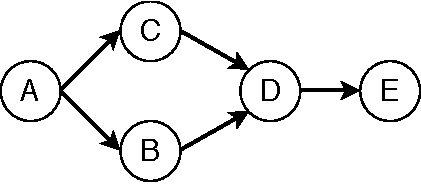
\includegraphics[width=70mm]{example-dataflow.pdf}
	\caption{Egy példa adatfolyam}
	\label{fig:example-dataflow}
\end{figure}

Az adatfolyamok áteresztőképességét triviálisan tudjuk növelni, ha csomópontokat valamilyen módszer szerint elosztjuk különböző feldolgozóegységek között. Ekkor azonban a konzisztens eredmények miatt szükséges valamilyen koordináció a csomópontok között. Továbbá ahhoz, hogy összetettebb műveleteket tudjuk elvégezni az adatfolyamokkal, szükség lehet iteratív algoritmusok végrehajtására, amikhez elengedhetetlen elemek a ciklusok. Az ilyen nagy áteresztőképességű, elosztott, iteratív elemeket tartalmazó, rövid válaszidővel rendelkező adatfolyamokban a csomópontok közötti koordináció kulcsfontosságú a rendszer hatékonyságához.

Erre ad egy megoldást az \emph{időzített adatfolyam} (IAF, timely dataflow)~\cite{DBLP:journals/cacm/MurrayMIIBA16} számítási modell. Az IAF egy olyan batch-es számításokat támogató számítási modell, ahol egy ciklikus adatfolyamokban a csomópontok között közlekedő minden adatrekordhoz egy virtuális időbélyeget (egész számok egy listáját) rendelünk. Az időbélyegek használatával lehetőség nyílik aszinkron adatfolyamok létrehozására úgy, hogy az esetlegesen szükséges szinkronizáció biztosítása is megoldható marad. Az IAF esetében lehetőség van arra, hogy a csomópontok értesüljenek arról, hogy már megkapták egy adott időbélyeghez tartozó összes adatrekordot. A cikkben~\cite{DBLP:journals/cacm/MurrayMIIBA16} leírt elosztott mechanizmus használatával garantálni lehet azt, hogy az értesítés valóban az adott időbélyeghez tartozó összes üzenet megérkezése után történjen. A ciklikus adatfolyamok támogatása pedig a hierarchikus időbélyegekkel lehetséges: a ciklusok kezdetén mindig egy újabb időbélyeget fűzünk hozzá a meglévő időbélyegekhez, amely a ciklus iterációnak számát jelöli. Tehát az ilyen hierarchikus időbélyegek első száma azt mutatja meg, hogy az adott rekord a bementi adatok közül melyik batch-be tartozik, az összes többi szám pedig a beágyazott ciklusok iterációinak számát jelölik.

\begin{figure}[ht]
	\centering
	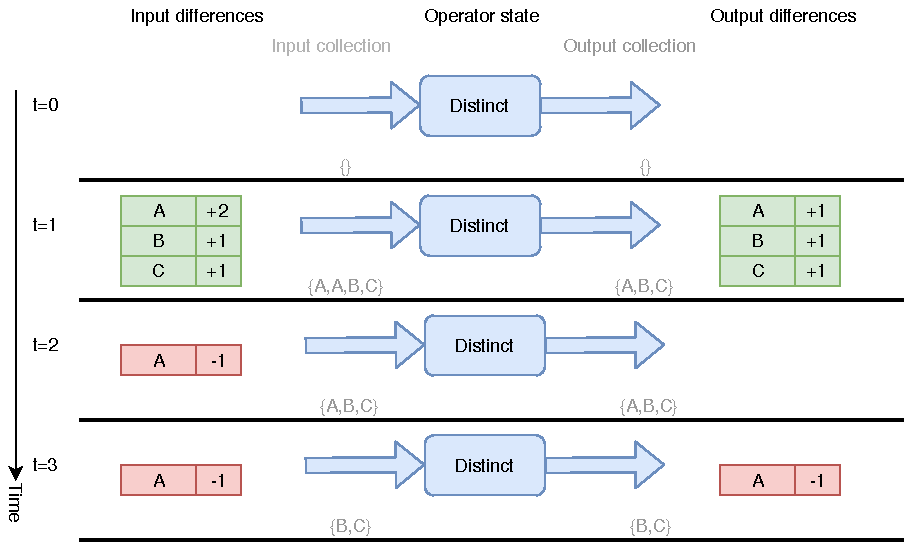
\includegraphics[width=150mm]{ddf_distinct.pdf}
	\caption{A \emph{distinct} operátor működése DAF esetében}
	\label{fig:ddf_distinct}
\end{figure}

Az időzített adatfolyam felett definiált inkrementális számítási modell a \emph{differenciális adatfolyam} (DAF, differential dataflow). A DAF célja adatpárhuzamos számítások inkrementális karbantartásának hatékony megvalósítása. Mivel a DAF-ok az adatrekordok mentén párhuzamosítanak, így a bemeneti adatok változása esetén minden csomópontnak elég a változott adatrekordokhoz tartozó eredményeket felülvizsgálni, így hatékonyan meg lehet határozni a kimenet változását is. Mivel az adatfolyamban csak a változásokat kommunikálják a csomópontok, így a csomópontok az őket követő csomópontoknak az adathalmaz méretéhez képest csak kevés adatrekordot továbbítanak. Egy DAF-ban használt \emph{distinct} operátor működése látható \aref{fig:ddf_distinct}.~ábrán. Figyeljük meg, hogy \emph{t=2} időpontban a bemenet változása nem vonja maga után a kimenet változását, így az operátor utáni csomópontoknak semmilyen számítást nem kell végezniük, garantáltan nem fog változni a kimenetük a DAF bemenetében történt változás hatására. Ezzel a módszerrel a változások okozta számítások minimalizálhatóak.

 
\subsection{Technológiák}
 
\subsubsection{Eclipse Modeling Framework (EMF)}

Az \emph{Eclipse Modeling Framework} egy keretrendszer, melyet modellvezérelt alkalmazásfejlesztésre terveztek. A keretrendszer része az Ecore metamodellező nyelv, melyet főleg doménspecifikus nyelvek és azok szerkesztőinek készítésére használják. Az Ecore a nyelv fejlesztői által definiált metamodell alapján számos hasznos eszköz (parser, serializer vagy akár triviális grafikus szerkesztő undo-redo támogatással) forráskódját képes legenerálni. \Aref{fig:ecore}.~ábrán látható az Ecore metamodellje, én csak a három legfontosabb elemét emelném ki:
\begin{itemize}
	\item Az \emph{EClass} példányai jelentik a modellezési nyelv osztályait.
	\item Az \emph{EAttribute} példányai jelentik a modellezési nyelv osztályainak attribútumait, az objektumok tulajdonságait.
	\item Az \emph{EReference} példányai pedig irányított kapcsolatot teremtenek a modellezési nyelv objektumai között.
\end{itemize}
Az EMF-en alapszik a modell alapú világ egy inkrementális lekérdezéseket és transzformációkat nyújtó keretrendszere, a \viatra~\cite{DBLP:journals/sosym/VarroBHHRU16}.

\subsubsection{.NET Modeling Framework (NMF)}
\label{sec:nmf}

Az EMF-hez hasonló modellezési keretrendszer a \emph{.NET Modeling Framework (NMF)}~\cite{DBLP:conf/icmt/Hinkel18}. Ahogy a neve is sugallja, .NET-ben (C\texttt{\#} nyelven) fejlesztett keretrendszer, azonban a .NET Core\footnote{\url{https://dotnet.microsoft.com}} futtatókörnyezetnek köszönhetően cross-platform keretrendszer.

\begin{figure}[ht]
	\centering
	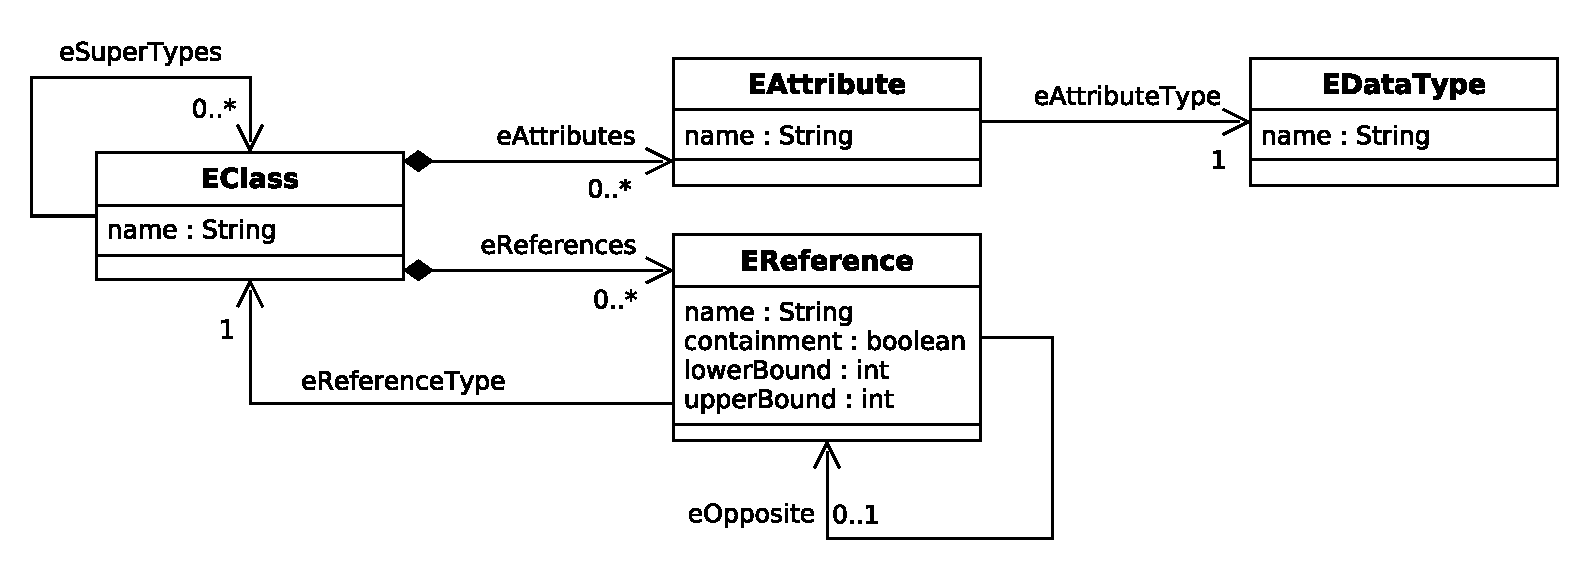
\includegraphics[width=150mm, keepaspectratio]{ecore}
	\caption{Az Ecore metamodellje}
	\label{fig:ecore}
\end{figure}

\subsubsection{Naiad}
\label{sec:naiad}

A Naiad~\cite{DBLP:conf/sosp/MurrayMIIBA13} a Microsoft Research Silicon Valley Lab\footnote{\url{https://www.microsoft.com/en-us/research/project/naiad/}} által fejlesztett IAF-t implementáló szoftverkönyvtár. A könyvtár által kínált szolgáltatások erősen beágyazottak a C\texttt{\#} által nyújtott infrastruktúrába: a felhasználók a  LINQ\footnote{\url{https://msdn.microsoft.com/en-us/library/bb308959.aspx}}-hoz hasonló módon definiálhatják az adatfolyam gráfot. Természetesen igény esetény egyedi csomópontokat is definiálhatunk. A Naiad szoftverkönyvtár a DAF-t implementáló keretrendszeren kívül tartalmaz kifejezetten gráf specifikus IAF operátorokat megvalósító keretrendszert is. A laboratórium bezárása, azaz 2014 ősze óta a Naiad nincs aktív fejlesztés alatt. 

\subsubsection{Timely Dataflow és Differential Dataflow}
\label{sec:differential-dataflow}

A IAF és DAF kidolgozásában és a Naiad implementációjában részt vevő egyik kutató saját projektjeként elkészítette az IAF\footnote{\url{https://github.com/frankmcsherry/timely-dataflow}} és DAF\footnote{\url{https://github.com/frankmcsherry/differential-dataflow}} implementációját Rust nyelven\footnote{\url{https://www.rust-lang.org/}}. Fontos előnye a Naiaddal szemben, hogy jelenleg is aktívan folyik a fejlesztése.

% !TeX spellcheck = hu_HU
% !TeX encoding = UTF-8
\chapter{Teljesítménymérési keretrendszer}\label{sec:keretrendszer}

A gráfalapú és a relációs adatbázis-kezelők teljesítményének és a használhatóságának összehasonlítása az adatbázis-kezelők fejleszőinek és a felhasználóinak is fontos információk forrása lehet. A fejlesztők megtudhatják, hogy a rendszerük mennyire hatékony a többi adatbázis-kezelőhöz képes, a felhasználók pedig a mérési eredmények révén több információ alapján választhatják ki a számukra megfelelő adatbázis-kezelőt.

A különböző adatbázisok és nyelvek összehasonlítása során szükség volt egy teljesítménymérési keretrendszerre, amely fókuszában a gráfadatbázisok állnak. Kiemelt szempont volt, hogy a keretrendszer lekérdezései általános formában legyenek definiálva, ne pedig egy adott lekérdezési nyelven megírt lekérdezésekkel. Ezen feltétel alapján a Linked Data Benchmark Council (LDBC)\footnote{A szervezet honlapja: \url{http://ldbcouncil.org}} szervezet Social Network Benchmark (SNB) keretrendszerét választottam, mert ez az elérhető legátfogóbb teljesítménymérési keretrendszer gráf információs rendszerek összehasonlító teljesítménymérésére.

Az LDBC egy európai uniós projekt keretében létrejött szervezet, amelynek célja teljesítménymérési keretrendszerek, munkafolyamatok létrehozása gráf vagy RDF alapú adatbázis-kezelő rendszerekhez, valamint az auditált mérési eredmények publikálása. Jelenleg több nagy cég támogatja a szervezetet\footnote{Az aktuális partnercégek listája megtekinthető a szervezet honlapján: \url{http://ldbcouncil.org/industry/members}}, mint például az Oracle, IBM, Intel, Neo4j és OpenLink Software (a Virtuoso gyártója).

\section{LDBC Social Network Benchmark}

Az LDBC SNB célja a gráf típusú adatbázis-kezelő rendszerek funkciójának széles körű tesztelése. Ehhez a keretrendszer egy szintetikus közösségi háló gráf alapú adatbázisát használja. Az adathalmaz sémája \aref{fig:dataschema}.~ábrán látható. A keretrendszer kétféle terhelési profilt tartalmaz.

Az úgynevezett \textit{Business Intelligence}~\cite{DBLP:conf/sigmod/ErlingALCGPPB15} (BI) terhelési profil olyan analitikus lekérdezéseket fogalmaz meg, amelyeknek a megválaszolásához az adathalmaz átfogó vizsgálata szükséges, például minden felhasználó üzeneteinek megszámolása. Ilyen lekérdezés például a legaktívabb, vagy éppen a legkevésbé aktív felhasználók megkeresése, vagy a baráti háromszögek megkeresése. A terhelési profil tervezése során gondosan figyeltek az olyan különböző kihívásokra, amelyeket az adatbázis-kezelő rendszereknek hatékonyan kell kezelni ahhoz, hogy nagyméretű adathalmazokon is megfelelő teljesítményt nyújtsanak. Ezek a kihívások a funkcionalitás széles köréből gyűjtötték össze: a relációs adatbázis-kezelőknél megfigyelt nehézségeken túl többek között a lekérdezőnyelvek kifejezőerejét, vagy a gráf specifikus lekérdezések komplexitását is vizsgálták ezen szempontrendszer felépítéséhez. A két teljesítménymérési profil közül a BI jött létre később, véglegesítése még jelenleg is folyamatban van.

Az \textit{Interactive}~\cite{DBLP:conf/grades/SzarnyasPAMPKEB18} profil lekérdezései pedig inkább egy, vagy néhány csomóponthoz kapcsolódó adat alapos vizsgálatát követelik meg. Az \textit{Interactive} profil lekérdezései három további csoportba sorolhatóak: 
\begin{itemize}
	\item Komplex lekérdezések (Complex reads, CR), 14 darab: Az adathalmaz számos pontját, általában egy ember ismerőseit és azok ismerőseit, valamint az ő aktivitásukat érintő lekérdezések. 
	\item Rövid lekérdezések (Short reads, SR), 7 darab: Egyszerű, általában öt csomópontnál nem többet érintő lekérdezések.
	\item Frissítések (Updates, U), 8 darab: Legfejlebb egy csomópont és néhány él beszúrása az adathalmazba.
\end{itemize}
A két terhelési profil két fontos tulajdonságának összehasonlítását mutatja \aref{fig:ldbc-graph-benchmarks}.~ábra: a feltételezett válaszidőt és a lekérdezés során megvizsgált adatmennyiséget. 
\begin{figure}[htb]
	\centering
	\begin{tikzpicture}[scale=1,thick]
	\tikzstyle{every node} = [align=center]
	
	\draw [stealth-stealth]
	(0,6.0) node (yaxis) [above left,rotate=90] {feltételezett válaszidő}
	|- (9.0,0) node (xaxis) [below left] {megvizsgált adatok mennyisége};
	
	\draw (0.5,0.5) rectangle ++(3.5,1.3) node[pos=0.5,text width=4cm] {LDBC SNB \\ Interactive \cite{DBLP:conf/sigmod/ErlingALCGPPB15}};
	\draw (4.5,3.4) rectangle ++(3.5,1.3) node[pos=0.5,text width=4cm] {LDBC SNB BI \\ \cite{DBLP:conf/grades/SzarnyasPAMPKEB18}};
	\end{tikzpicture}
	\caption{A teljesítménymérési profilok karakterisztikája.}
	\label{fig:ldbc-graph-benchmarks}
\end{figure}

Ahhoz, hogy a különböző rendszerek teljesítményét átfogóan lehessen elemezni, a keretrendszer támogatja az adathalmaz skálázását is. Az adathalmaz skálázási együtthatóját (scale factor, SF) a CSV\footnote{Comma-Separated Values} formátumban tárolt adathalmaz gigabájtban számolt mérete adja. A keretrendszer által előre konfigurált skálázási együtthatók a következők: 0.1, 0.3, 3, 10, 30, 100, 300, 1000. A különböző skálázási együtthatójú adathalmazok méretének szabályozása az adathalmazban szereplő emberek számának megadásával történik, ennek megfelelően generálódik a hálózat többi része. A mérésekhez használt SF1-es adathalmazban 11 ezer, az SF3-asban 27 ezer, az SF10-esben 73 ezer ember szerepel~\cite{LDBC_SNB}.

Az LDBC SNB lekérdezéseinek specifikációja tartalmaz egy szemléltető ábrát, és a lekérdezés szabadszöveges megfogalmazását is. Ennek köszönhetően nem csak az adatbázis-kezelő rendszerek, de a lekérdezési nyelvek összehasonlítására is alkalmas a keretrendszer.

\subsection{A teljesítménymérés munkafolyamata}

A keretrendszer munkafolyamatát \aref{fig:workflow}.~ábra mutatja be. A munkafolyamatban négy típusú összetevő van: \textit{(1)} a keretrendszerhez kapcsolódó szoftvermodulok és a lekérdezések forráskódja, \textit{(2)} eljárás, \textit{(3)} emberek által definiált adat és \textit{(4)} generált adat. Az összetevőket továbbá két csoportba sorolhatjuk az alapján, hogy az elkészítésük vagy végrehajtásuk a keretrendszer fejlesztőinek (LDBC SNB munkacsoport) vagy felhasználóinak (Adatbázis-kezelők fejlesztői, felhasználói) a feladata.

A keretrendszer fejlesztőinek feladatai:
\begin{itemize}
	\item A \textit{lekérdezések specifikációnak}\footnote{\url{https://github.com/ldbc/ldbc_snb_docs}} elkészítése és karbantartása~\cite{LDBC_SNB}
	\item Az adathalmazokat és lekérdezések paramétereit \textit{generáló alkalmazás} (DATAGEN)\footnote{\url{https://github.com/ldbc/ldbc_snb_datagen}} elkészítése
	\item A megvalósítások ellenőrzése és a teljesítménymérést végző \textit{alkalmazás keretrendszer} (DRIVER)\footnote{\url{https://github.com/ldbc/ldbc_snb_driver}} elkészítése
	\item A \textit{referenciaimplementáció} elkészítése
	\item Az egyes lekérdezések elvárt eredményét tartalmazó adathalmaz, azaz a \textit{referencia validációs adathalmaz} elkészítése
\end{itemize}
Ezen részfolyamatok elkészülte után a felhasználók elkezdhetik megvalósítani a saját összetevőket. A DATAGEN modullal a felhasználók generálhatnak adott méretű adathalmazt, illetve a hozzá tartozó lekérdezés paramétereket. A dolgozat készítése során a Sparksee implementációt tekintettem referenciaimplementációnak.

A felhasználók által végzett munkát további két csoportba lehet osztani: az implementáció ellenőrzése és a teljesítménymérés. Mindkettőhöz szükséges az adott adatbázis-kezelőhöz tartozó szoftvermodulok és lekérdezések implementációja. A szoftvermodulok közé tartoznak az adatok betöltését, a lekérdezések futtatását végző és az eredményeket a DRIVER számára feldolgozható formátumra konvertáló modulok. Az ellenőrzés lépései ezek után az alábbiak:
\begin{itemize}
	\item Az \textit{ellenőrzési beállítások} (például mennyi lekérdezést futtason a keretrendszer) és a \textit{lekérdezés paraméterek} alapján az \textit{eszközhöz tartozó validációs adatok} (a lekérdezések eredményeinek) előállítása
	\item Az eredmények összevetése a referencia validációs adathalmazzal: ha az eredmény megegyezik a referencia validációs adathalmazzal, akkor következhet a teljesítménymérés, ellenkező esetben a hibákat javítani kell és újra ellenőrizni az implementációt
\end{itemize}
A felhasználói beállítások sok finomhangolási lehetőséget biztosítanak, például mennyi végrehajtási szálon fusson egyidőben az ellenőrzés, összesen mennyi lekérdezést végezzen el, illetve az egyes lekérdezések ellenőrzését egyenként lehet engedélyezni vagy tiltani, stb..

\begin{figure}[h]
	\centering
	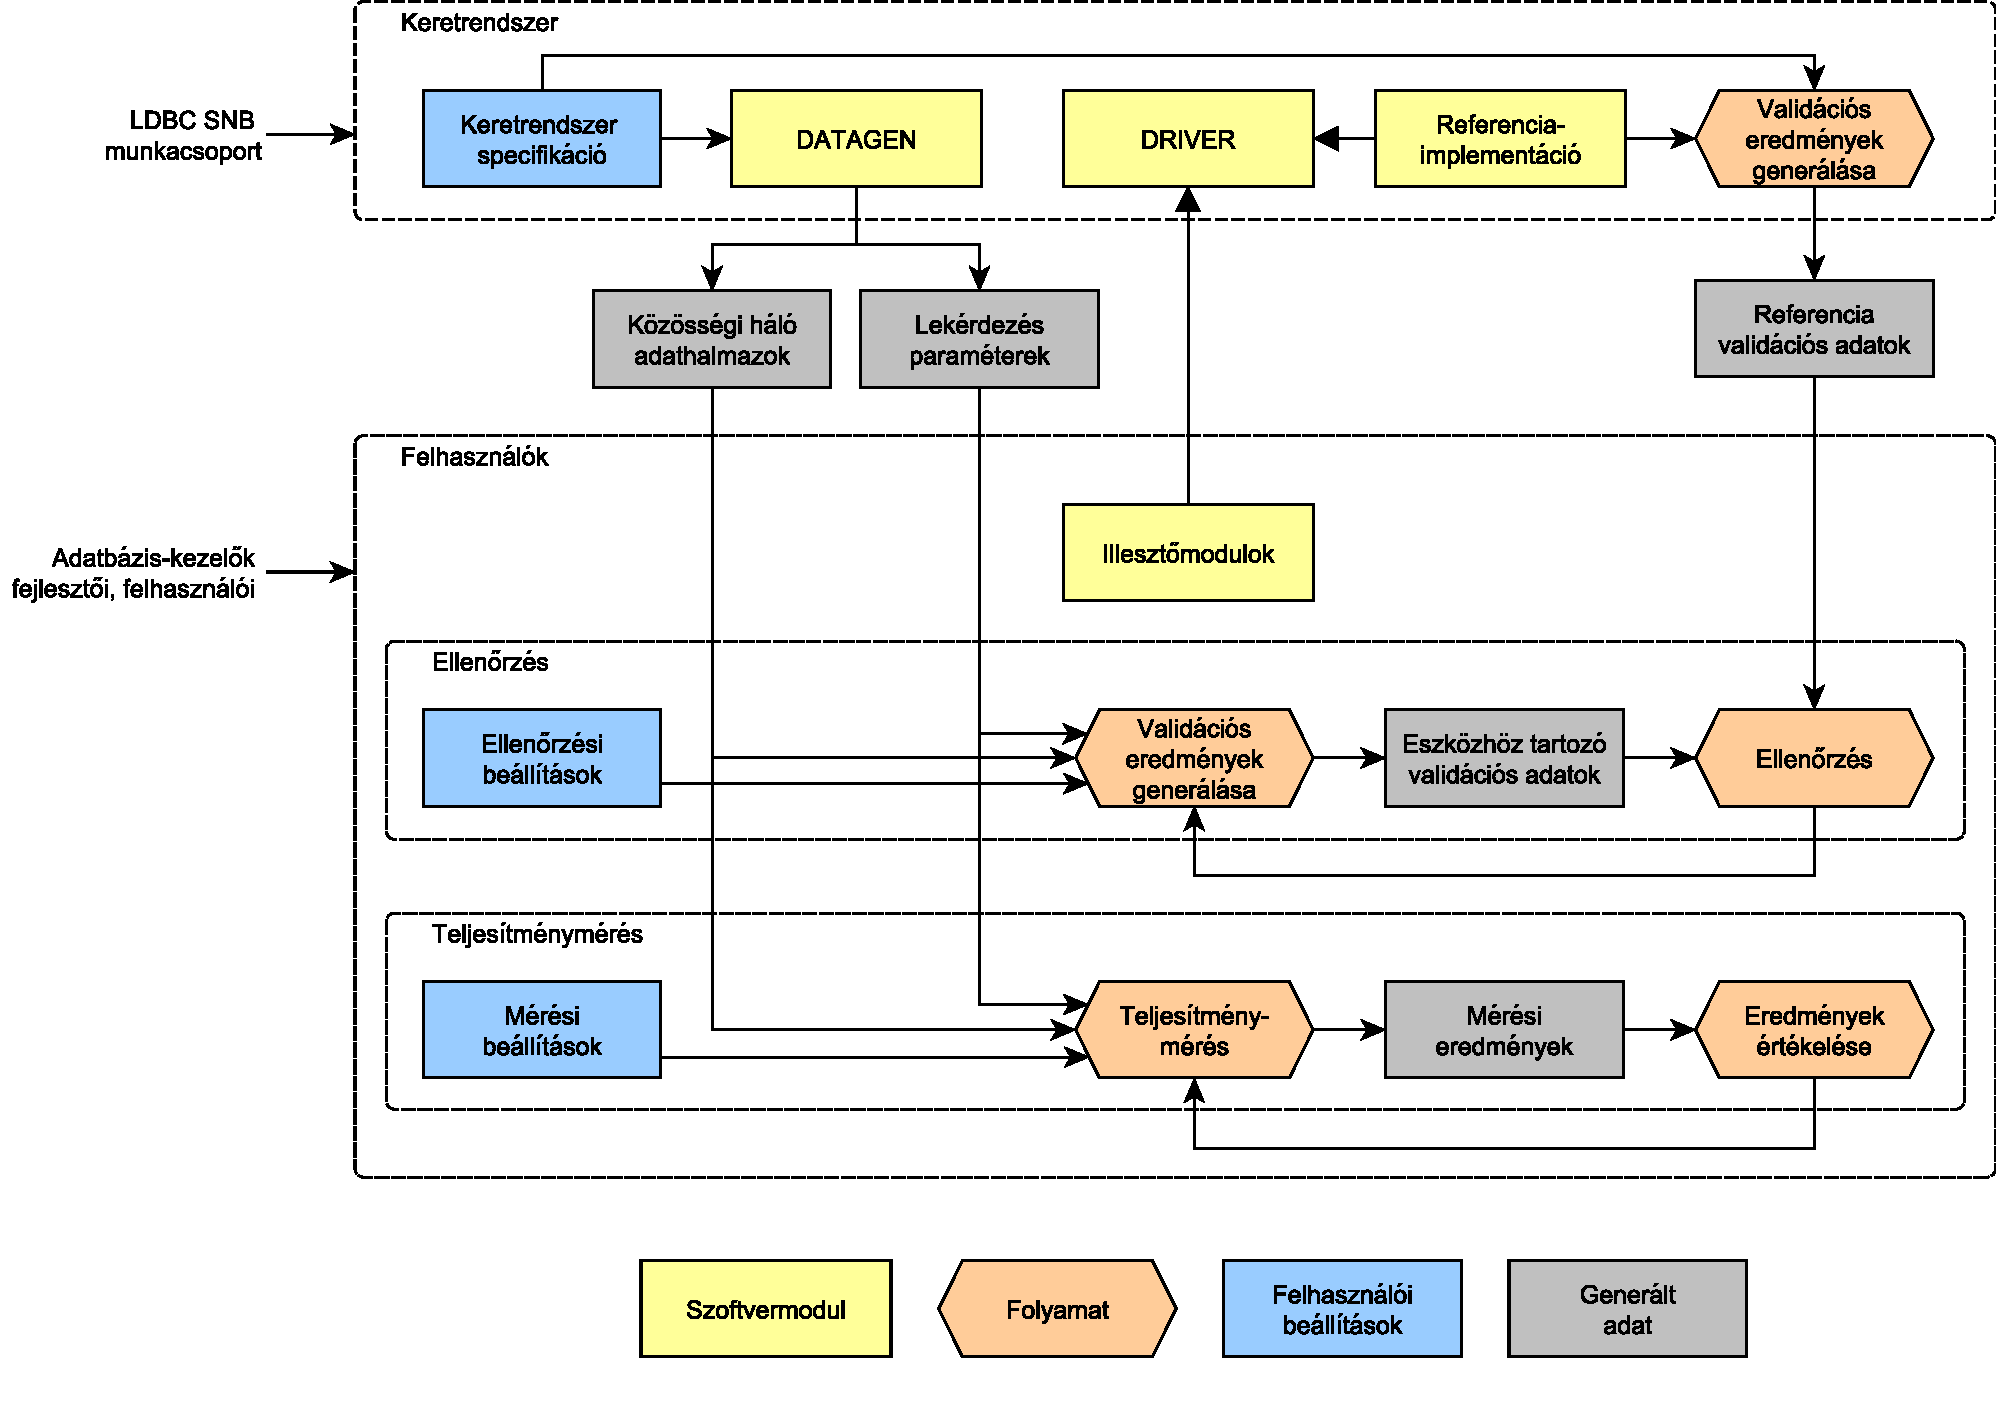
\includegraphics[width=\linewidth]{workflow.pdf}
	\caption{A teljesítménymérési keretrendszer munkafolyamata}
	\label{fig:workflow}
\end{figure}

Ha az implementáció átment az ellenőrzésen, akkor a teljesítménymérés a következő lépés. A teljesítménymérés lépései hasonlóak az ellenőrzés lépéseihez:
\begin{itemize}
	\item A \textit{mérési beállítások} és a lekérdezés paraméterek alapján a teljesítményérés futtatásával a \textit{mérési eredmények} elkészítése
	\item Az eredmények értékelése és esetleges új mérés indítása (például nagyobb méretű adathalmazon)
\end{itemize}

\section{Teljesítménymérési keretrendszer bővítése}
A dolgozat készítése során az LDBC SNB-t bővítettem a \textit{Business Intelligence} terhelési profil SPARQL, és az \textit{Interactive} terhelési profil SPARQL és Cypher implementációjával, ezzel bővítve ki a keretrendszerrel lemérhető adatbázis-kezelők halmazát. Ezen felül implementáltam egy Gremlin-t támogató adatbázis-kezelőkhöz használható adatbetöltő alkalmazást.
\subsection{Business Intelligence terhelési profil}

A Business Intelligence terhelési profil lekérdezéseit SPARQL nyelven készítettem el. A lekérdezéseknek nem létezett SPARQL megvalósítása. A lekérdezések komplexitásából adódóan az implementálás során sok esetben a nyelv kifejezőerejét is próbára tették. A 25-ös lekérdezést nem is lehet szabványos SPARQL-ben megvalósítani, mert nem támogatja a legrövidebb utak keresését. A következőkben bemutatom az általam legérdekesebb, vagy legnagyobb kihívásokat, amelyekkel az implementáció készítése során szembesültem.

\paragraph{NULL érték kezelése}
A megszokott lekérdezési nyelvekkel ellentétben a SPARQL-ben nincsenek a megszokott értelemben vett NULL értékek: a változók lehetnek kötöttek, vagy kötetlenek, azaz vagy tartozik hozzájuk egy érték vagy nem. Az egyszerű gráfminták csak akkor illeszkednek egy adott részgráfra, ha minden változó kötött, azaz mindegyikhez tartozik egy érték. Ez alól az egyetlen kivétel a \keyword{OPTIONAL} kulcsszóval megadott opcionális gráfminták, mert az azokban megadott változók lehetnek kötetlenek. Fontos megjegyezni, hogy egy opcionális gráfmintában megadott változókat tekintve vagy mind kötött, vagy egyik sem, azaz az ilyen minták esetében is igaz az, hogy csak akkor illeszkednek, ha minden változójuk kötött. Például a \listref{sparql-null}~kódrészletben szereplő SPARQL lekérdezés eredményében az \textit{?a}, \textit{?b} és \textit{?c} változók mindig kötöttek lesznek, míg a \textit{?i} és \textit{?j} közül vagy mindkettő kötött, vagy mindkettő kötetlen lesz az eredmény egy sorában.

\vspace{1.5ex}

\noindent\begin{minipage}{\textwidth}
\begin{lstlisting}[frame=single, morekeywords={SELECT},label=listing:sparql-null, caption=Példa az OPTIONAL kulcsszóra]
SELECT
	?a, ?b, ?c, ?i, ?j
WHERE
{
	?a predicate1 ?b .
	?b predicate2 ?c .
	OPTIONAL {
		?a predicate3 ?i .
		?b predicate4 ?j 
	}
}
\end{lstlisting}
\end{minipage}

\paragraph{Nevesített gráfminták hiánya}
A SPARQL nem támogatja nevesített gráfminták létrehozását, így nem lehet többször felhasználható gráfmintákat létrehozni. Ez kifejezetten kényelmetlenné teszi a 15-öshöz hasonló lekérdezések leírását. A 15-ös lekérdezés grafikus specifikációja látható a \figref{bi15}~ábrán. Jól látható, hogy az azonos országból származó barátok megszámolására kétszer is szükség van, azonban mivel a gráfmintát nem lehet elnevezni, így a lekérdezésben is kétszer kellett leírni ugyanazt a gráfmintát. Összetett gráfmintáknál a több példány szinkronban tartása kényelmetlen és sok hibalehetőséget hordoz.

\begin{figure}[!ht]
	\centering
	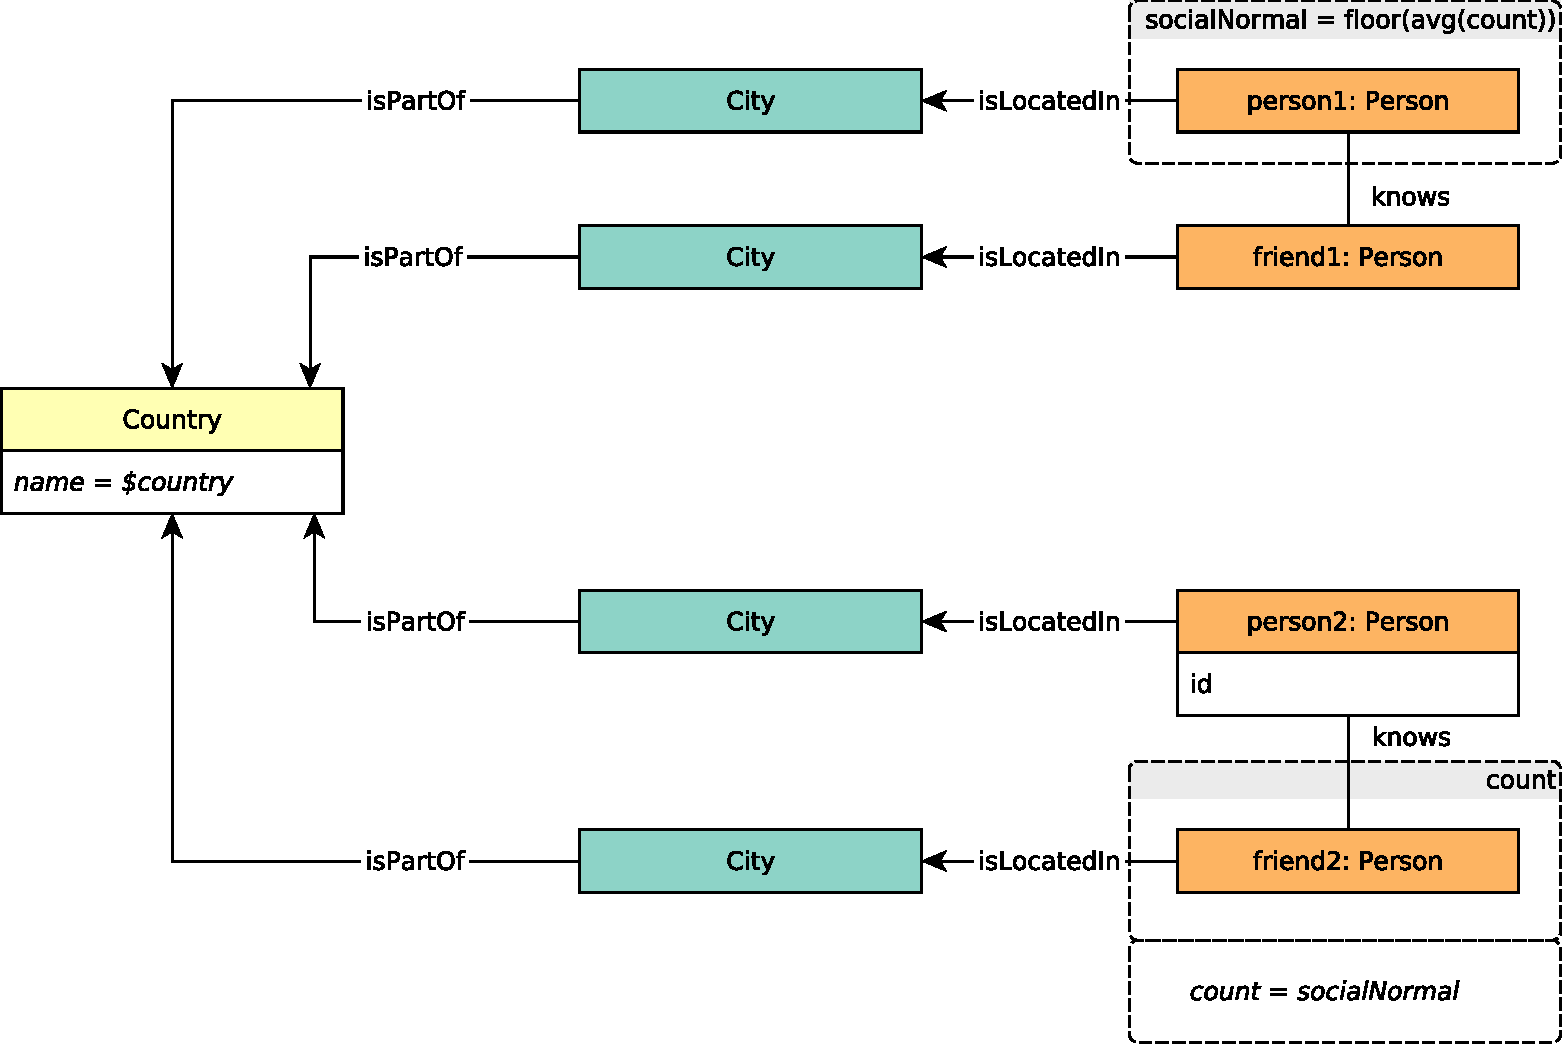
\includegraphics[width=\textwidth, keepaspectratio]{bi-read-15}
	\caption[]{A BI15-ös lekérdezés}
	\label{fig:bi15}
\end{figure}

\paragraph{Deklarációk hiánya}
Mivel SPARQL nyelvben a változók deklarálása a változóra történő első hivatkozás, így a hosszabb lekérdezések esetében az esetleges elgépelésekkel újabb, természetesen nem kívánt változókat deklarálhatunk. Ezen a nyelv megváltoztatása nélkül egy megfelelő SPARQL szerkesztővel lehet segíteni, azonban a dolgozat készítése közben nem sikerült ilyen eszközt találni, a SPARQL szintaxis kiemelését is csak néhány egyszerű szöveges szerkesztő támogatja. A deklarációk hiánya egyébként több másik lekérdezőnyelvben is problémát jelent (pl. Datalog, Cypher, VQL).

\paragraph{Utak hosszának definiálása}
Bár SPARQL-ben van lehetőség változó hosszú útvonal-kifejezések leírására, azonban a Cypher \lstinline{x..y} alakú kifejezésével megegyező nyelvi konstrukciót nem tartalmaz a SPARQL. Ez a nyelvi konstrukció azonban szükséges a \figref{bi16}~ábrán látható 16-os lekérdezés megvalósításához, mivel a benne lévő út hossza a lekérdezése paramétere. Ennek ellenére a 16-os lekérdezéshez készítettem egy olyan implementációt, amelyben az útvonal-kifejezést a keretrendszer szoftvermodulja generálja le és illeszti be a SPARQL lekérdezésbe, így megteremtve a lehetőségét a nem triviális útvonal-kifejezéseket tartalmazó lekérdezések összehasonlítására.

\begin{figure}[!ht]
	\centering
	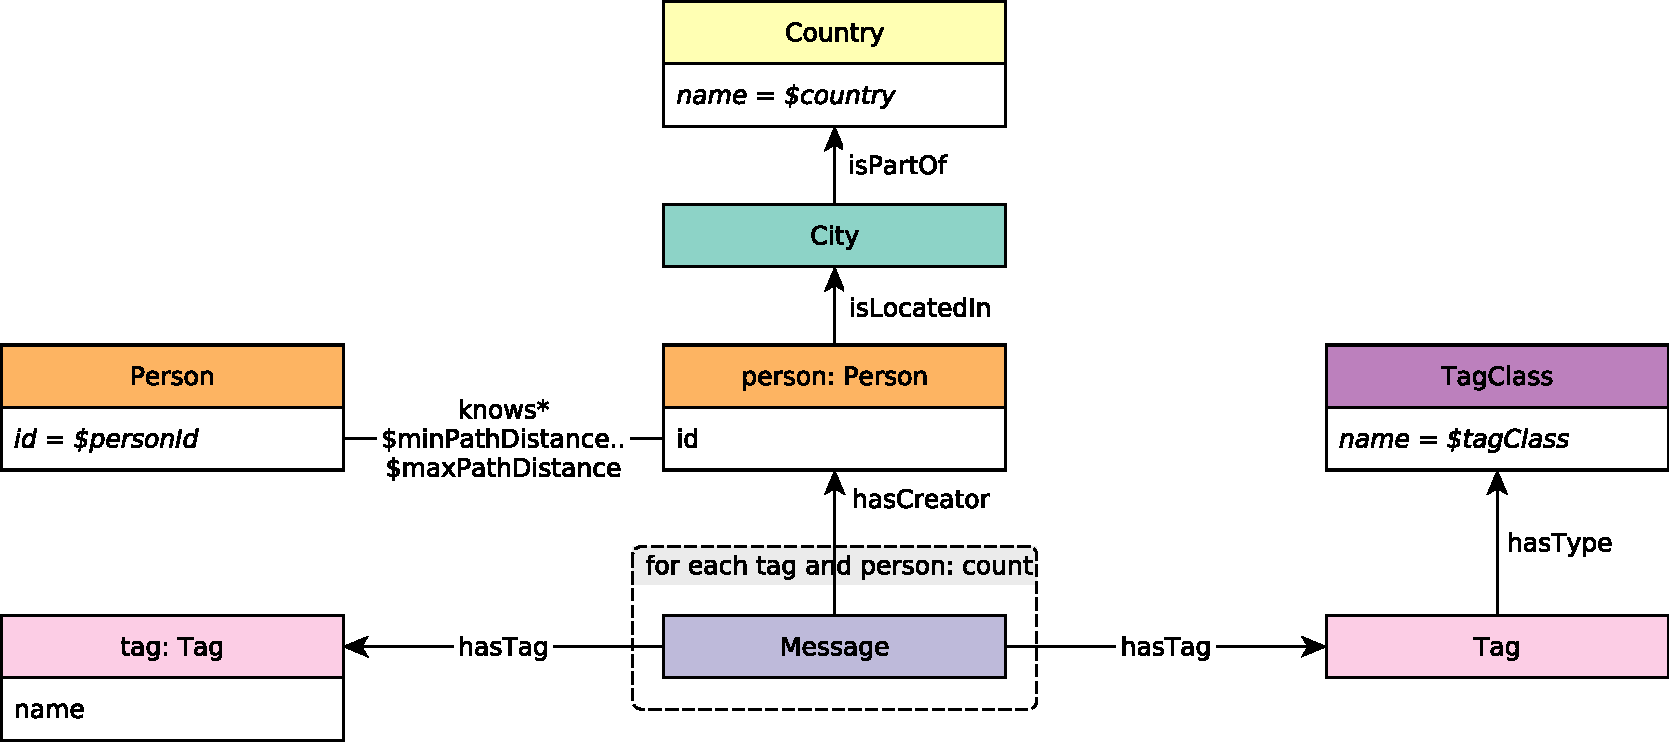
\includegraphics[width=\textwidth, keepaspectratio]{bi-read-16}
	\caption[]{A BI16-os lekérdezés}
	\label{fig:bi16}
\end{figure}

\subsection{Interactive terhelési profil}
\subsubsection{SPARQL implementációk}

Az interaktív terhelési profil CR és SR lekérdezéseinek két implementációja (az egyik az LDBC SNB implementációja, a másik pedig egy szabadon elérhető implementáció\footnote{A Waterloo-i Egyetemen fejlesztett implementáció: \url{https://github.com/anilpacaci/ldbc_snb_implementations}}~\cite{DBLP:conf/grades/PacaciZLO17}) is létezett, de több probléma is volt velük:
\begin{itemize}
	\item A lekérdezések csak a Virtuoso adatbázis saját SPARQL dialekutásban voltak elérhetők. A Virtuoso SPARQL dialektusa több olyan konstrukciót tartalmaz, ami az eredeti SPARQL nyelvhez képest tömörebb és kifejezőbb lekérdezések írását teszi lehetővé. Ezek átírása szabványos SPARQL nyelvre nem-triviális lépéseket igényel, és nem is lehetséges minden esetben.
	\item A lekérdezések specifikációi az implementáció elkészülte óta pontosítva, javítva lettek, így néhány lekérdezés hibássá vált.
	\item Néhány lekérdezés nem a leghatékonyabb struktúrájú volt.
\end{itemize}
Ezen okok miatt a lekérdezések teljes újraimplementálása mellett döntöttem, nem próbáltam meg a meglévő lekérdezéseket átalakítani. A munka során a specifikáció alapján implementáltam\footnote{SPARQL implementáció: \url{https://github.com/ldbc/ldbc_snb_implementations/pull/51}} 27 darab (12 db CR, 7 db SR, 8 db U) lekérdezést SPARQL nyelven.

A CR13 lekérdezéshez szükséges egy legrövidebb út megtalálása, a CR14 lekérdezéshez az összes legrövidebb út megtalálása és súlyozása az érintett csomópontok alapján. Ezeket a funkciókat a SPARQL szabvány nem tartalmazza, így ezeket a lekérdezéseket nem implementáltam. Az implementáció elkészítése során \textit{(1)} implementáltam a 27 darab lekérdezést SPARQL nyelven, \textit{(2)} implementáltam a lekérdezések végrehajtását és a lekérdezések eredményének konvertálását végző szoftvermodulokat Java nyelven, \textit{(3)} a keretrendszert használva sikeresen végrehajtottam az implementáció ellenőrzését.

A munkát nehezítette, hogy a lekérdezések specifikációi sok esetben pontosításra, vagy kiegészítésre szorultak, vagy az adathalmaz régebbi változtatásai miatt frissíteni kellett azokat. Tehát a terhelési profil lekérdezéseinek implementálása közben a terhelési profilhoz kapcsolódó dokumentációkat is frissítettem, kiegészítettem, így megkönnyítve más felhasználóknak a saját lekérdezéseik és moduljaik elkészítését.

\subsubsection{Cypher implementációk}

A terhelési profilhoz nem volt elkészítve a Cypher implementáció, azonban egy másik nyílt forráskódú projektben\footnote{A Stanford Egyetemen fejlesztett implementáció: \url{https://github.com/PlatformLab/ldbc-snb-impls}} a lekérdezések jelentős része implementálásra került. Bár ezek a lekérdezések sem voltak hibátlanok, minőségük jelentősen jobb volt, mint a SPARQL-ben létező lekérdezéseké, így ezeket fel tudtam használni a végleges implementáció\footnote{Cypher implementáció: \url{https://github.com/ldbc/ldbc_snb_implementations/pull/57}} elkészítéséhez. A SPARQL implementációhoz hasonló módon itt is három részre lehet osztani az elvégzett munkát: \textit{(1)} a meglévő lekérdezések implementációjának ellenőrzése és javítása, illetve a hiányzók implementálása Cypher nyelven, \textit{(2)} a szükséges szoftvermodulok implementációja, \textit{(3)} az implementáció ellenőrzése. Fontos megjegyezni, hogy a jelenleg szabványosítás alatt álló openCypher nyelv nem tartalmazza a legrövidebb utak kifejezésére szolgáló nyelvi konstrukciókat (pl. \texttt{shortestPath} és \texttt{allShortestPath}), így CR13 és CR14 lekérdezések csak Cypher (és nem openCypher) nyelven értelmezhetőek.

\subsubsection{Gremlin adatbetöltő}
A dolgozat készítése során megpróbálkoztam a Cypher for Gremlin\footnote{\url{https://github.com/opencypher/cypher-for-gremlin}} projekt felhasználásával a keretrendszert kiterjeszteni a Gremlin-t támogató adatbázis-kezelőkre is, azonban nem sikerült minden technikai problémát megoldani a dolgozat elkészültéig. Még a triviális Cypher lekérdezésekből generált Gremlin lekérdezések is igen nagy méretűek, a generált jellegből fakadóan az elnevezések nem intuitívak, így a lekérdezések futtatása, a hibakeresés vagy éppen az eredmények megfelelő formátumra való konvertálása sem triviális feladat. \listref{cypher-example}~kódrészletben szereplő Cypher lekérdezésből az alábbi Gremlin lekérdezést állítja elő a projekt:
\begin{lstlisting}[frame=single,language=Java]
g.V().as('p').hasLabel('Person').as('p').choose(__.select('p').is(neq('  cypher.null')).outE('KNOWS').inV().as('f').hasLabel('Person'), __.select('p').is(neq('  cypher.null')).outE('KNOWS').inV().as('f').hasLabel('Person'), __.constant('  cypher.null').as('f')).select('p', 'f').group().by(__.select('p').choose(neq('  cypher.null'), __.choose(__.values('name'), __.values('name'), __.constant('  cypher.null')), __.constant('  cypher.null'))).by(__.fold().project('p.name', 'count(f)').by(__.unfold().select('p').choose(neq('  cypher.null'), __.choose(__.values('name'), __.values('name'), __.constant('  cypher.null')), __.constant('  cypher.null'))).by(__.unfold().select('f').is(neq('  cypher.null')).count())).unfold().select(values)
\end{lstlisting}
Az implementáció nem teljes körű, de az adatok betöltését végző szoftvermodul funkcionalitását tekintve elkészült, az adatok betöltésére alkalmas.

% !TeX spellcheck = hu_HU
% !TeX encoding = UTF-8
\chapter{Transformation Tool Contest (TTC)}
\label{sec:ttc}

\newcommand{\ttcyedscale}{0.55}

Az adatok transzformációja az alkalmazások egy széles rétegében központi szerepet tölt be. Ezen alkalmazások erősen függnek az elérhető transzformációs eszközök által nyújtott szolgáltatásokon és azok hatékonyságán. Az alkalmazások fejlesztőinek a számukra legalkalmasabb eszköz kiválasztása nehéz feladat, mivel számos modell- és gráftranszformációs eszköz érhető el manapság. Még a legtapasztaltabb szakemberek is általában egy vagy két eszközt ismernek alaposan, a többiről pedig csak kevés ismeretük van.
Az évente megrendezésre kerülő Transformation Tool Contest (TTC)\footnote{A TTC hivatalos weboldala: \url{https://www.transformation-tool-contest.eu/}} célja, hogy összehasonlítsa a különböző transzformációs eszközök kifejezőerejét, használhatóságát és teljesítményét. 2007 óta minden évben különböző, a valós felhasználások inspirálta feladatokat tesznek közzé, amelyekre bármilyen eszközzel lehet megoldást készíteni. A feladatok a transzformációk felhasználásának széles köréből merítenek ötleteket, többek között:
\begin{itemize}
	\item modell szinkronizáció és egyesítés (merge)
	\item modellek és transzformációk validációja
	\item szemantikus keresés
	\item programok manipulációja és transzformációja
\end{itemize}
Az utóbbi két évben pedig mindig volt egy feladat az \emph{inkrementális nézetkarbantartás} témakörében is. A 2018-as feladatok egyike az LDBC SNB egy egyszerűsített sémája feletti két nézet inkrementális karbantartása volt. A következőkben ezt a feladatot ismertetjük részletesen.

\section{TTC Közösségi háló feladat}

Az TTC 2018 \emph{Közösségi háló} feladatának (Social Media case) egyszerűsített LDBC SNB adatsémáját mutatja be \aref{fig:ttc-schema}.~ábra.
A modellben tehát lehetnek felhasználók (\textsf{User}), akik különböző üzeneteket (\textsf{Submission}) írhatnak (\textsf{submitter} és \textsf{submissions} kapcsolatok): bejegyzéseket (\textsf{Post}) és hozzászólásokat (\textsf{Comment}).
A felhasználók továbbá kedvelhetik (\textsf{likedBy} és \textsf{likes} kapcsolatok) a hozzászólásokat. A felhasználók között lehetőség van barátságok kifejezésére (\textsf{friends} kapcsolatok) is. A hozzászólásokat a felhasználók egy már meglévő üzenethez fűzhetik hozzá (\textsf{comments} és a \textsf{commented} kapcsolatok), tehát a hozzászólásokat reprezentálhatjuk olyan fákkal, ahol egy hozzászólás őse mindig az az üzenet, amelyikre reagáltak az adott hozzászólással. Ekkor belátható, hogy minden ilyen fában pontosan egy bejegyzés lesz, ami a fa gyökere, mivel hozzászólásokat csak meglévő üzenetekhez lehet fűzni. A feladatban a modellek frissítései csak bővítő jellegűek, azaz már meglévő objektumok és kapcsolatok nem törlődnek a modellből, csak újak adódnak hozzá.

Mivel a feladat kiinduló adatmodellje az NMF-fel (\ref{sec:nmf}. szakasz) egyszerűen beolvasható, ezért adott volt a lehetőség a feladatok Naiaddal történő megoldására, mivel a modellek beolvasásához használhattam az NMF-et. Ennek következtében a feladat kiváló lehetőségnek bizonyult
a DAF számítási modell (\ref{sec:differential-dataflow}. szakasz) és 
a Naiad szoftverkönytár (\ref{sec:naiad}. szakasz)
használhatóságának tesztelésére és teljesítménymérésére.

\begin{figure}
	\centering
	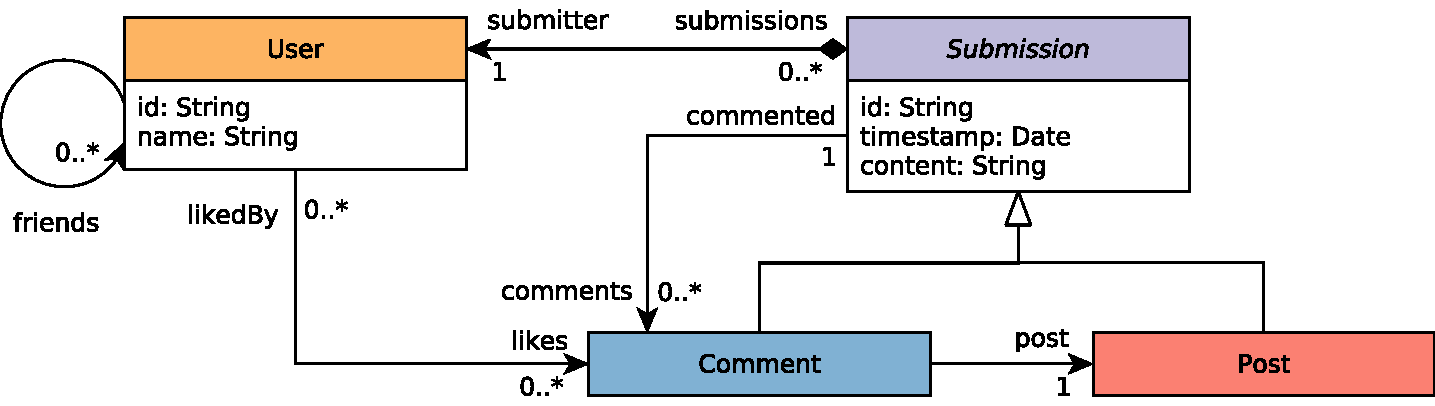
\includegraphics[scale=\ttcyedscale, keepaspectratio]{ttc_schema}	
	\caption{A TTC 2018 Közösségi háló feladatának adatsémája}
	\label{fig:ttc-schema}
\end{figure}

\subsection{A Q1 lekérdezés}

\begin{figure}[ht]
	\centering
	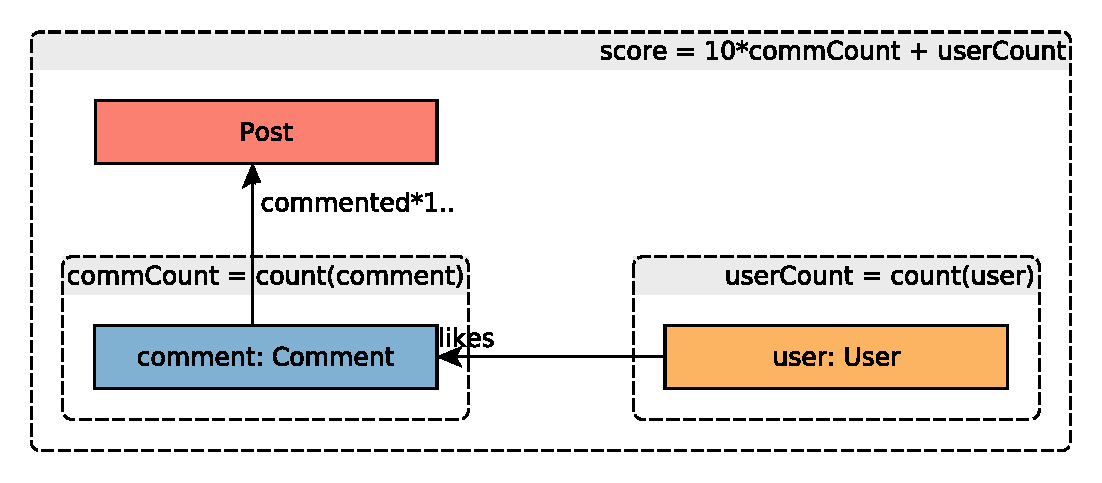
\includegraphics[scale=\ttcyedscale, keepaspectratio]{t1}	
	\caption{A Q1 lekérdezés grafikus ábrázolása}
	\label{fig:ttc-t1}
\end{figure}

Ebben a lekérdezésben a bejegyzéseket pontozzuk a hozzájuk tartozó hozzászólások és kedvelések alapján. A bejegyzések minden hozzájuk tartozó hozzászólás után 10, a bejegyzéshez és hozzászólásokhoz tartozó kedvelések után pedig további 1 pontot kapnak. Egy felhasználó kedvelései több pontot is érhetnek, ha azok különböző üzenetekhez tartoznak. Az így pontozott bejegyzések közül keressük a három legnagyobb pontszámmal rendelkező bejegyzést. Egyenlő pontszámok esetén a korábban létrehozott bejegyzés élvez elsőbbséget. A lekérdezés grafikus szemléltetése látható \aref{fig:ttc-t1}.~ábrán.

A lekérdezés egy konkrét eredményét láthatjuk \aref{fig:ttc-example}.~ábrán. Az ábra felső részén látható a kiindulási állapot \textsf{p1} bejegyzéssel, \textsf{c1} és \textsf{c2} hozzászolásokkal és \textsf{u1}, \textsf{u2}, \textsf{u3} és \textsf{u4} felhasználókkal. A \textsf{p1} bejegyzéshez tartozó pontszám az alábbi részpontszámokból adódik össze:
\begin{itemize}
	\item 20 pont \textsf{c1} és \textsf{c2} hozzászólások miatt
	\item 2 pont a \textsf{c1} hozzászólásra adott kedvelések (\textsf{u2} és \textsf{u3} felhasználó) miatt
	\item 3 pont a \textsf{c2} hozzászólásra adott kedvelések (\textsf{u1}, \textsf{u2} és \textsf{u3} felhasználó) miatt
\end{itemize}
Összesen tehát 25 pontot rendelünk ebben az esetben a \textsf{p1} bejegyzéshez. Az ábra alsó felében a vastagon szedett nyíl jelenti a frissítés által hozzáadott új kedvelést. Ez a kedvelés a \textsf{c2} hozzászóláshoz tartozó kedvelés pontjait növeli meg 3-ról 4-re, így a \textsf{p1} bejegyzés pontszáma 26-ra módosul.

\subsection{A Q2 lekérdezés}

\begin{figure}[ht]
	\centering
	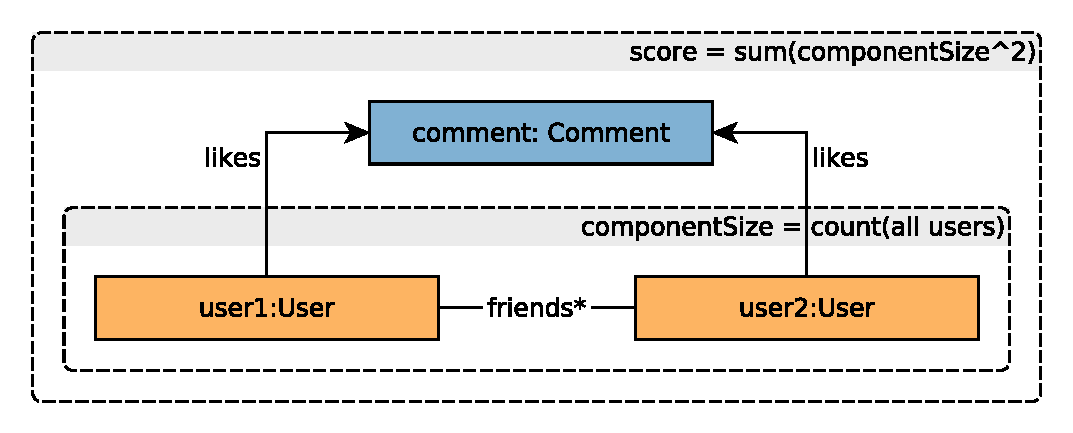
\includegraphics[scale=\ttcyedscale, keepaspectratio]{t2}	
	\caption{A Q2 lekérdezés grafikus ábrázolása}
	\label{fig:ttc-t2}
\end{figure}

Ebben a lekérdezésben azokat a hozzászólásokat keressük, amelyek a felhasználók legnagyobb csoportjai által kedveltek. A felhasználó csoportokat a barátság kapcsolaton keresztül azonosítjuk: egy adott hozzászólást kedvelő felhasználók közül egy csoportba tartoznak azok a felhasználók, akik a barátság kapcsolatokon keresztül összefüggő komponenseket (strongly connected components, SCC) alkotnak.
Tehát egy olyan gráfban keresünk összefüggő komponenseket, ahol a hozzászólást kedvelő felhasználók a csúcsok, és a közöttük lévő barátság kapcsolatok pedig az élek. Az összefüggő komponensek azonosítása után összegezzük a komponensek méretének négyzetösszegét. A lekérdezés grafikus szemléltetése látható \aref{fig:ttc-t2}.~ábrán.

\Aref{fig:ttc-example}.~ábrán szintén láthatjuk a lekérdezés egy konkrét eredményét. A \textsf{p1} bejegyzés pontszáma a következő részpontszámokból adódik össze:
\begin{itemize}
	\item $2 \times 2 = 4$ pont a \textsf{c1} hozzászólást kedvelő felhasználók miatt, mivel ők egy 2 elemű komponenst alkotnak
	\item $2 \times 2 + 1 \times 1 = 5$ pont a \textsf{c2} hozzászólást kedvelő felhasználók miatt, mivel egy 1 elemű (\textsf{u1}) és egy 2 elemű (\textsf{u3} és \textsf{u4}) komponenst alkotnak
\end{itemize}
Összesen tehát a \textsf{p1} bejegyzéshez 9 pontot rendelünk. Az ábra alsó felében, a frissítés után látható, hogy a \textsf{c2} hozzászólást kedvelő felhasználók immár egy 4 elemű komponenst alkotnak, tehát a \textsf{c2}-höz tartozó részpontszám 16-ra ($4 \times 4$) változik, így a \textsf{p1} bejegyzés pontszáma pedig 20 pontra változik.

\begin{figure}
	\centering
	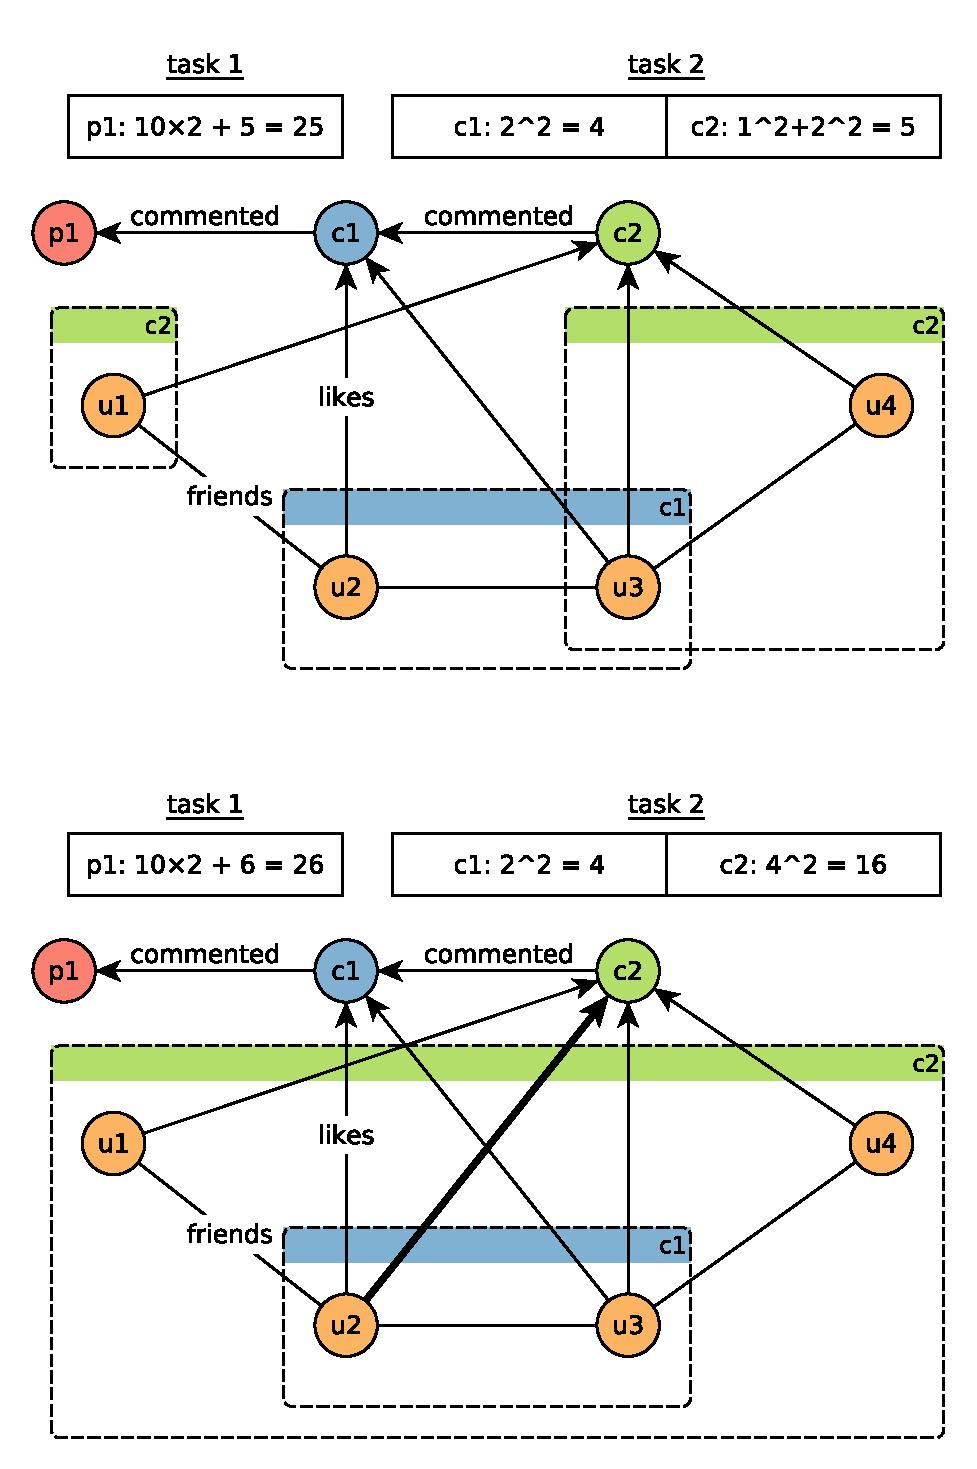
\includegraphics[scale=\ttcyedscale, keepaspectratio]{ttc-example}	
	\caption{A lekérdezések eredményének grafikus ábrázolása. A második modellben a vastag él az újonnan hozzáadott élet jelöli.}
	\label{fig:ttc-example}
\end{figure}

\subsection{Megoldás ismertetése}

A megoldás során a Naiad könyvtárban rendelkezésre álló DAF keretrendszert használtam. A keretrendszer a relációs lekérdezőnyelvekben használatos operátorok (\keyword{SELECT}, \keyword{JOIN}, \keyword{DISTINCT}, \keyword{COUNT}, \keyword{SUM} stb.) DAF alapú megvalósításán túl további operátorokat is definiál. A megoldásaim három olyan operátort használnak, amelyek túlmutatnak vagy nem megszokottak a relációs lekérdezőnyelvek világán:
\begin{itemize}
	\item \uline{\texttt{FixedPoint}:} A \texttt{FixedPoint} operátor használatával definiálhatjuk a DAF-ban említett ciklusokat. A ciklusok létrehozásakor meg kell adni azt a DAF-ot, amit a ciklus belsejében szeretnénk végrehajtani, valamint a DAF bemenetének számító adatforrást. Az operátor nevével összhangban egy iterációban addig hajtja végre a beágyazott DAF-ot, amíg annak kimenete két iteráció között megváltozik. A beágyazott DAF bemenetének típusa természetesen meg kell egyezzen a kimenetének típusával, így lehet ciklusként végrehajtani. Az operátor által létrehozott ciklust az úgynevezett \texttt{LoopContext} objektum azonosítja. Az operátor használatára a Q1 esetében a bejegyzésekhez tartozó hozzászólások (tranzitív lezártak) keresésekor, a Q2 esetében pedig az összefüggő komponensek keresésekor volt szükség.
	\item \uline{\texttt{EnterLoop}:} A \texttt{FixedPoint} operátor alapértelmezetten csak egy adatforrást támogat, azonban lehetőség van a ciklusokon belül több adatforrást is használni az \texttt{EnterLoop} operátor használatával. Bemenete egy adatforrást reprezentáló objektum és egy \texttt{LoopContext} objektum, kimenete pedig egy olyan adatforrást reprezentáló objektum, ami már használható a beágyazott DAF-ban is. Használatát a \texttt{FixedLoop} használatának szükségessége indokolta.
	\item \uline{\texttt{CoGroupBy}:} A Naiad által nyújtott DAF keretrendszer nem definiál külső illesztéseket végrehajtó operátorokat, azonban a \texttt{CoGroupBy} operátor nagyon hasonló szemantikával rendelkezik, használatával megvalósíthatóak a külső illesztések. Az operátor bemenete két adatforrás és a hozzájuk tartozó kulcsderiváló függvények. Az operátor a kulcsok szerint csoportosítja a két adatforrásból érkező adatrekordokat, így \textsf{<key, list1, list2>} hármasokat állít elő belőlük, ahol a \textsf{key} a közös kulcs, \textsf{list1} és \textsf{list2} pedig rendre az első és a második adatforrásból a  kulcshoz tartozó adatrekordok listája. A \texttt{CoGroupBy} operátort a hozzászólásokhoz tartozó kedvelések megszámolására használtam.
\end{itemize}
A Q1 lekérdezés differenciális adatfolyamának szemléltetése \aref{fig:q1-ddffig}.~ábrán látható, amelyeken megfigyelhető a \texttt{FixedPoint} és a \texttt{EnterLoop} operátorok kapcsolata.
% !TeX spellcheck = hu_HU
% !TeX encoding = UTF-8
\newcommand{\plotscale}{0.6}

\chapter{Kiértékelés} \label{sec:kiertekeles}
\section{Adatbázis-kezelő rendszerek teljesítményének mérése az LDBC SNB keretrendszerrel}
\subsection{Motiváció}

Bár a relációs adatbázis-kezelők a mai napig a legelterjedtebb adatbázis-kezelők\footnote{\url{https://db-engines.com/en/ranking}}, az újgenerációs adatbázis-kezelők változatos funkcionalitásaikkal és lekérdezőnyelveikkel újra és újra megpróbálják felvenni a versenyt velük. A gráf alapú adatbázis-kezelők az utóbbi években jelentős fejlődésen mentek keresztül, ezzel jelentősen növelve népszerűségüket\footnote{\url{https://db-engines.com/en/ranking_categories}}. Ahhoz, hogy eldöntsük, fel tudják-e venni a versenyt a relációs adatbázis-kezelőkkel, szükséges a teljesítményük összehasonlítása is. 

A dolgozatban összehasonlított alkalmazások összetettsége bőven meghaladja azt a szintet, hogy a teljesítményüket a forráskódok elemzése alapján össze lehetne hasonlítani. Ezért a tudományban már bizonyított módon kísérletek, mérések alapján próbálom összehasonlítani őket.

A dolgozatban összehasonlított technológiák kiválasztásában leghangsúlyosabb szempont a lekérdezőnyelveik voltak:
\begin{itemize}
	\item SQL: Régóta használt, a legelterjedtebb relációs adatbázis-kezelők szabványos nyelve.
	\item SPARQL: A dolgozatban bemutatott gráf alapú lekérdezőnyelvek közül a legteljesebb matematikai háttérrel rendelkező, szemantikailag legtisztább lekérdezőnyelv.
	\item Cypher: A gráf alapú lekérdezőnyelvek között az egyik legnépszerűbb lekérdezőnyelv, véleményem szerint az egyik legintuitívabb és legkifejezőbb nyelv.
\end{itemize}

\begin{table}[h]
	\centering
	\begin{tabular}{|l|r|r|r|}
		\toprule
		\multicolumn{1}{l}{Nyelv} & \multicolumn{1}{l}{BI karakterszám} & \multicolumn{1}{l}{Int. karakterszám}& \multicolumn{1}{l}{Összesen} \\
		\midrule
		Cypher & 13\,657 & 19\,021 & 32\,678 \\
		SPARQL & 32\,417 & 43\,548 & 75\,965 \\
		SQL    & 30\,417 & 14\,563 & 44\,980 \\
		\bottomrule
	\end{tabular}
	\caption{A különböző nyelveken megírt BI és Interactive lekérdezések karakterszáma fehér szóközök (szóközök, tabulátor és újsor karakterek) nélkül}
	\label{tab:char-count}
\end{table}

A Cypher kifejezőerejét és tömörségét \aref{tab:char-count}.~táblázat is alátámasztja. A lekérdezések SQL-ben 37\%, SPARQL-ben pedig 132\%-kal több karaktert tartalmaznak, mint a Cypherben írt lekérdezések.

Annak érdekében, hogy átfogó képet kapjak az elérhető gráf információs rendszerek teljesítményéről, egy összetett mérési sorozatot terveztem és futtattam.

\subsection{Business Intelligence terhelési profil}

A mérés során három implementációval végeztem méréseket a BI terhelési profil felhasználásával:

\begin{enumerate}
	\item PostgreSQL: a PostgreSQL relációs adatbázis-kezelő rendszer.
	\item Sparksee: a Sparksee tulajdonsággráf adatbázis-kezelő rendszer.
	\item \stardog: egy szemantikus adatbázis.
\end{enumerate}

A meg nem nevezett adatbázis-kezelő rendszer eredményeit anonimizált módon adom közre. Ennek oka, hogy ugyan a lekérdezések minden esetben \emph{validáltak} (azaz helyes eredményeket biztosítanak), de nem \emph{auditáltak} (azaz a rendszerek gyártói nem vizsgálták meg az implementációt, így nem garantált, hogy az optimális teljesítményt biztosít).

A teljesítménymérés során az egyes implementációk válaszidejét és skálázhatóságát mértem. Válaszidő alatt a lekérdezés végrehajtásának elkezdésétől a lekérdezésre adott válasz teljes megérkezéséig eltelt időt értjük. A skálázhatóság alatt a válaszidő adathalmaz méretétől függő változását értem. 

\subsubsection{Mérési elrendezés}

A dolgozat készítése során végzett mérések egy számítógépen történtek az LDBC SNB keretrendszer driver szoftvermoduljának 0.3.1-es verziójának felhasználásával. A számítógép 8 fizikai processzormagot (Intel(R) Xeon(R) E5-2673), és 256 GB memóriát tartalmaz. A háttértár egy SCSI interfészen kapcsolt 128GB-os SSD lemez. Az operációs rendszere 64 bites Ubuntu 16.04.

A PostgreSQL 10.5-ös verzióját használtam az SQL mérésére. A meg nem nevezett adatbázis-kezelő méréséhez az utóbbi 6 hónapban kiadott verziót használtam. A driver és opcionálisan a meg nem nevezett adatbázis-kezelő rendszer az OpenJDK 1.8.0\_181-es verzióját használták. Az adatbázis-kezelő konfigurációját a dokumentációja alapján próbáltam optimalizálni, azonban az anonimitás miatt a pontos beállításokat nem közölhetem.

A lekérdezések \aref{sec:keretrendszer}.~fejezetben leírt módon kerültek ellenőrzésre az SF1-es adathalmazokon.
A teljesítménymérés során a rendszereken először futtattam 100 darab bemelegítő (warmup) lekérdezést, majd 250 lekérdezés válaszidejét mértem meg. A lekérdezések véletlenszerűen választottak és végrehajtásuk szekvenciálisan, átlapolódás nélkül történt. 

\begin{figure}
	\centering
	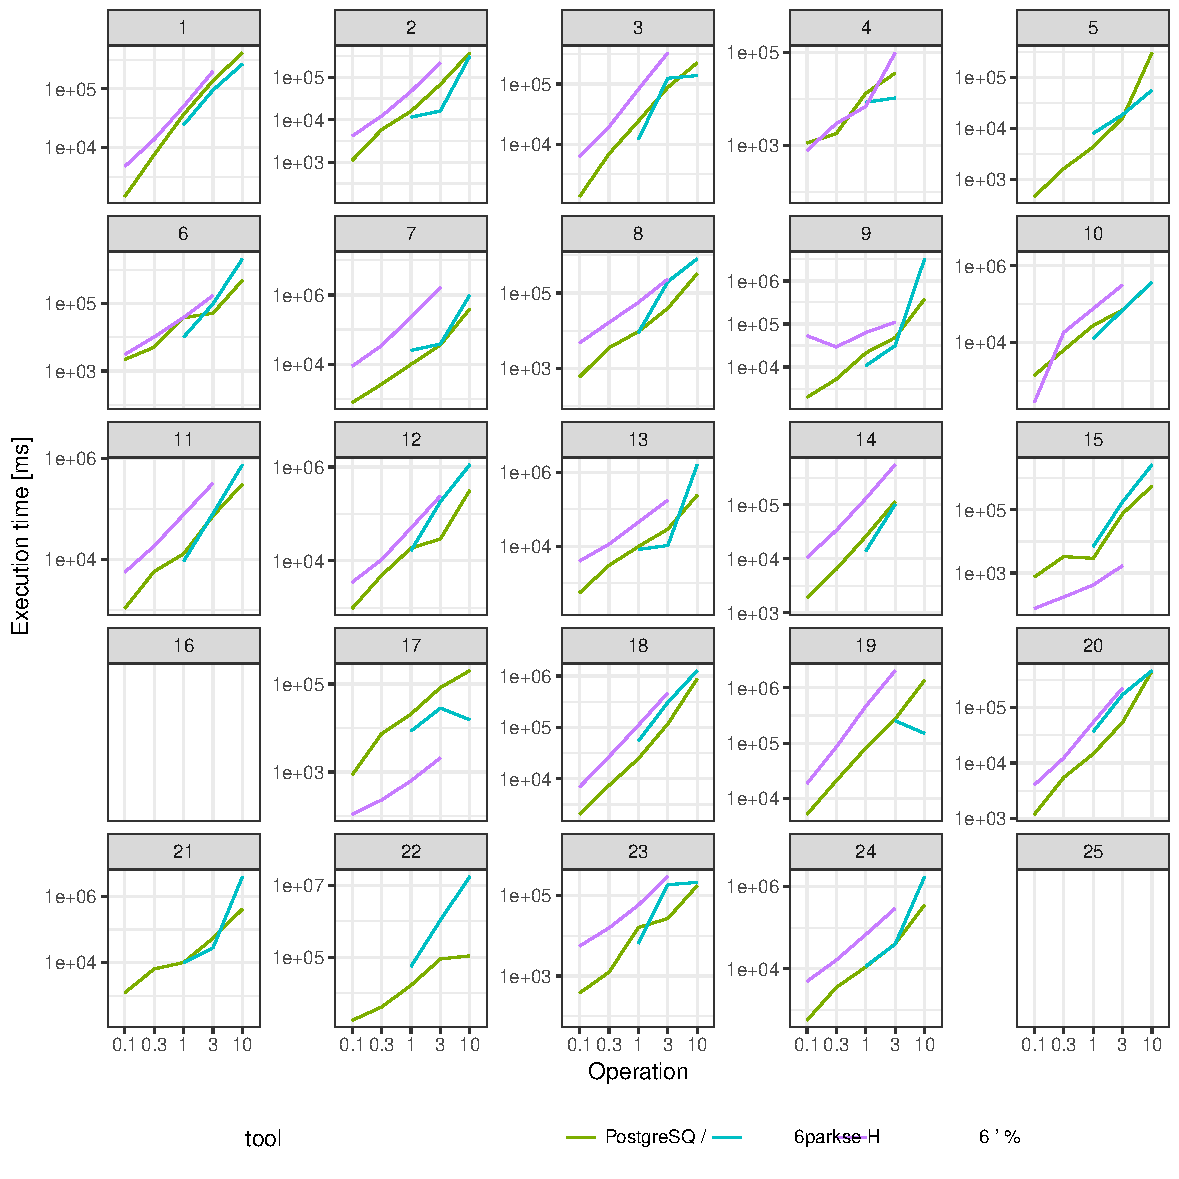
\includegraphics[width=\textwidth]{bi-execution-times}
	\caption{A lekérdezések összesített mérési eredményei}
	\label{fig:bi-execution-times}
\end{figure}

\subsubsection{Eredmények értékelése}

A mérési eredményeket \aref{fig:bi-execution-times}.~ábra tartalmazza. A profil bonyolultságát jól szemlélteti, hogy több olyan lekérdezést (4-es és 14-es) is tartalmaz, amelyeket egyik adatbázis-kezelő sem tudott végrehajtani a legnagyobb adathalmazon, továbbá számos lekérdezés válaszideje elérte a több tíz másodpercet mindhárom rendszer esetében már az SF3-as adathalmazon is (1-es, 3-as, 11-es, 14-es, 15-ös, 18-as, 19-es, 22-es lekérdezés). Egyértelműen látszik, hogy nehezebben megfogalmazható és összetettebb lekérdezéseket tartalmaz, mint az Interactive profil.

Érdemes megfigyelni, hogy a Sparksee két lekérdezés (17-es és 19-es) esetében is jobb válaszidőt produkált az SF10-es adathalmazon, mint az SF3-as adathalmazon.

\subsection{Interactive terhelési profil}
A mérés során négy implementációval végeztem méréseket az Interactive terhelési profil komplex lekérdezéseinek felhasználásával:

\begin{enumerate}
	\item PostgreSQL: a PostgreSQL relációs adatbázis-kezelő rendszer.
	\item Sparksee: a Sparksee tulajdonsággráf adatbázis-kezelő rendszer.
	\item \virtuoso: egy szemantikus adatbázis.
	\item \stardog: egy szemantikus adatbázis.
\end{enumerate}

A két meg nem nevezett adatbázis-kezelő rendszer eredményeit a BI terhelési profilhoz hasonlóan anonimizált módon adom közre a már említett ok miatt: a lekérdezések \textit{validáltak}, de nem \textit{auditáltak}.

A teljesítménymérés során az egyes implementációk válaszidejét és skálázhatóságát mértem. Válaszidő alatt a lekérdezés végrehajtásának elkezdésétől a lekérdezésre adott válasz teljes megérkezéséig eltelt időt értjük. A skálázhatóság alatt a válaszidő adathalmaz méretétől függő változását értjük. 

\subsubsection{Mérési elrendezés}

A dolgozat készítése során végzett mérések egy számítógépen történtek az LDBC SNB keretrendszer driver szoftvermoduljának 0.3.1-es verziójának felhasználásával. A számítógép 16 fizikai processzormagot (Intel(R) Xeon(R) Platinum 8167M CPU @ 2.00GHz), és 236 GB memóriát tartalmaz. A háttértár egy SCSI interfészen kapcsolt 128GB-os SSD lemez. Az operációs rendszere 64 bites Ubuntu 18.04.

A PostgreSQL 10.5-ös\footnote{(PostgreSQL 10.5 (Ubuntu 10.5-0ubuntu0.18.04) on x86\_64-pc-linux-gnu, compiled by gcc (Ubuntu 7.3.0-16ubuntu3) 7.3.0, 64-bit)} verzióját használtam az SQL implementációk mérésére.

A meg nem nevezett adatbázis-kezelők méréséhez (a BI profil méréséhez hasonlóan) az utóbbi 6 hónapban kiadott verziókat használtam. A driver és a meg nem nevezett adatbázis-kezelők közül a Java nyelvű rendszerek az OpenJDK 1.8.0\_181-es verzióján futottak. Az adatbázis-kezelők konfigurációját a dokumentációjuk alapján próbáltam optimalizálni, azonban az anonimitás miatt a pontos beállításokat nem közölhetem.

A lekérdezések a rövid lekérdezésekkel és a frissítésekkel együtt \aref{sec:keretrendszer}.~fejezetben leírt módon kerültek ellenőrzésre az SF1-es adathalmazokon, több mint 13 ezer lekérdezés eredményének összehasonlításával.

\begin{table}
	\centering
	\begin{tabular}{|l|r|r|r|}
		\toprule
		Skálázási tényező & SF1 & SF3 & SF10 \\
		\midrule
		PostgreSQL & 1000 & 1000 & 1000 \\
		Sparksee & 1000 & 1000 & 1000 \\
		\virtuoso & 1000 & 1000 & 1000 \\
		\stardog & 1000 & 750 & 40 \\
		\bottomrule
	\end{tabular}
	\caption{A implementációk mérése során futtatott lekérdezések száma}
	\label{tab:query-count}
\end{table}

A mérés során a lekérdezéseket különböző behelyettesítési paraméterekkel futtattam \aref{tab:query-count}.~táblázat szerinti darabszámban. Annak érdekében, hogy a mérések összideje ne legyen túl nagy, több korlátozást is kellett tennem. A \stardog mérése során már SF3 esetében is csökkenteni kellett a lekérdezések számát, illetve az SF10-es adathalmazon egyáltalán nem mértem le az \stardog-t, mert nem futott le egy lekérdezés sem.

Mindegyik eszköz mérésnél a különböző méretű adathalmazokon legalább 20-szor futott egy lekérdezés (különböző paraméterekkel).


\subsubsection{Eredmények értékelése}

A mérési eredményeket \aref{fig:results-interactive-aggregated}.~ábra tartalmazza.

\begin{figure}
	\centering
	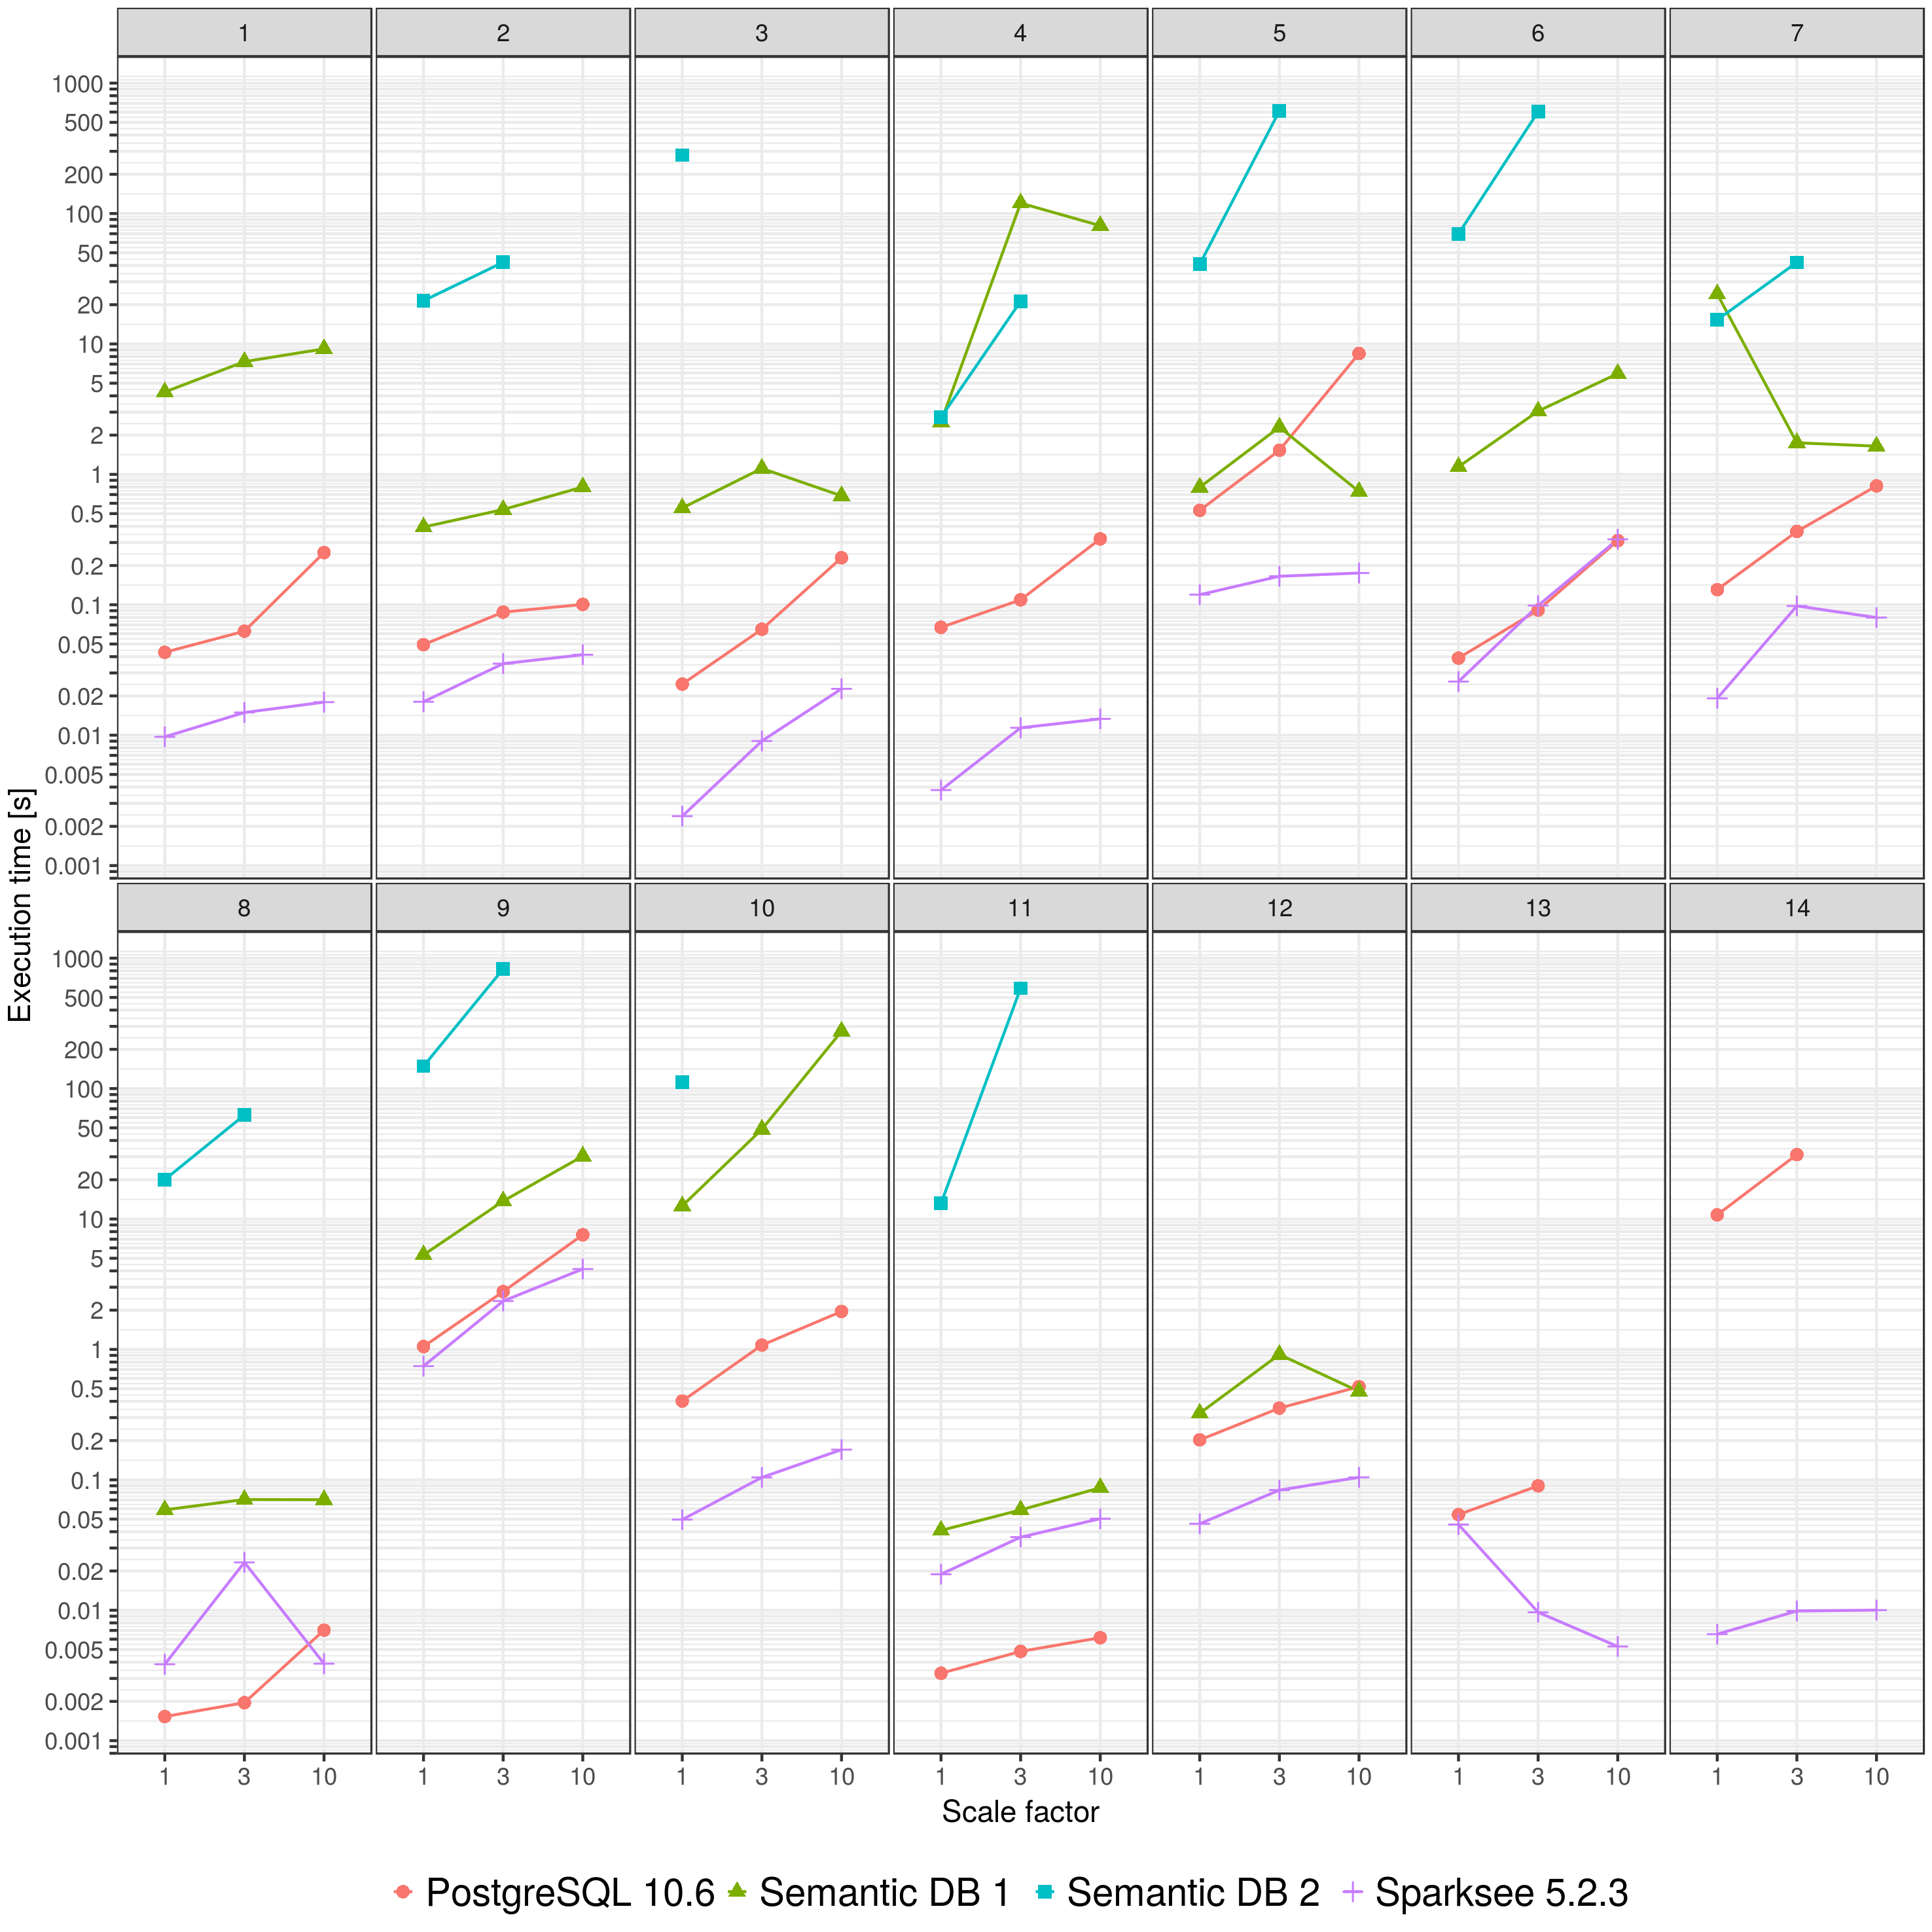
\includegraphics[scale=\plotscale]{results/results-interactive-aggregated.png}
	\caption{A lekérdezések összesített mérési eredményei}
	\label{fig:results-interactive-aggregated}
\end{figure}

Az egyik legfontosabb eredmény, hogy a lekérdezések többségénél a legjobb eredményt a Sparksee érte el. Hozzá hasonlóan jól teljesített a PostgreSQL, ezzel bizonyítva, hogy a relációs adatbázis-kezelők a közel 50~éves fejlődésnek köszönhetően manapság is a leghatékonyabb adatbázis-kezelők közé tartoznak.

Megfigyelhető, hogy a 3-as, 4-es, 5-ös és 12-es lekérdezéseknél az \virtuoso eszköz kisebb átlagos válaszidővel rendelkezik az SF10-es adathalmazon, mint az SF3-as adathalmazon. A lekérdezések specifikációjából~\cite{LDBC_SNB} kiderül, hogy az említett lekérdezésekben szerepel összetett aggregáció. Az említett lekérdezéseken kívül összetett aggregáció csak a 6-os lekérdezésben van, amelynél azonban nem figyelhető meg ilyen fajta teljesítmény-növekedés. A jelenségre nem sikerült konkrét hipotézist felállítani, de az említett komplex aggregációnak köze lehet a jelenséghez.

A 7-es lekérdezésnél szintén megfigyelhető a teljesítmény javulása a nagyobb adathalmazokon. Abban azonban más jellegű ez a javulás, mert az SF1 adathalmaz után, az SF3-as adathalmaznál figyelhető meg jelentős javulás, míg az SF3 adathalmaz után az SF10-es adathalmaznál csak minimális mértékű.

\begin{figure}
	\centering
	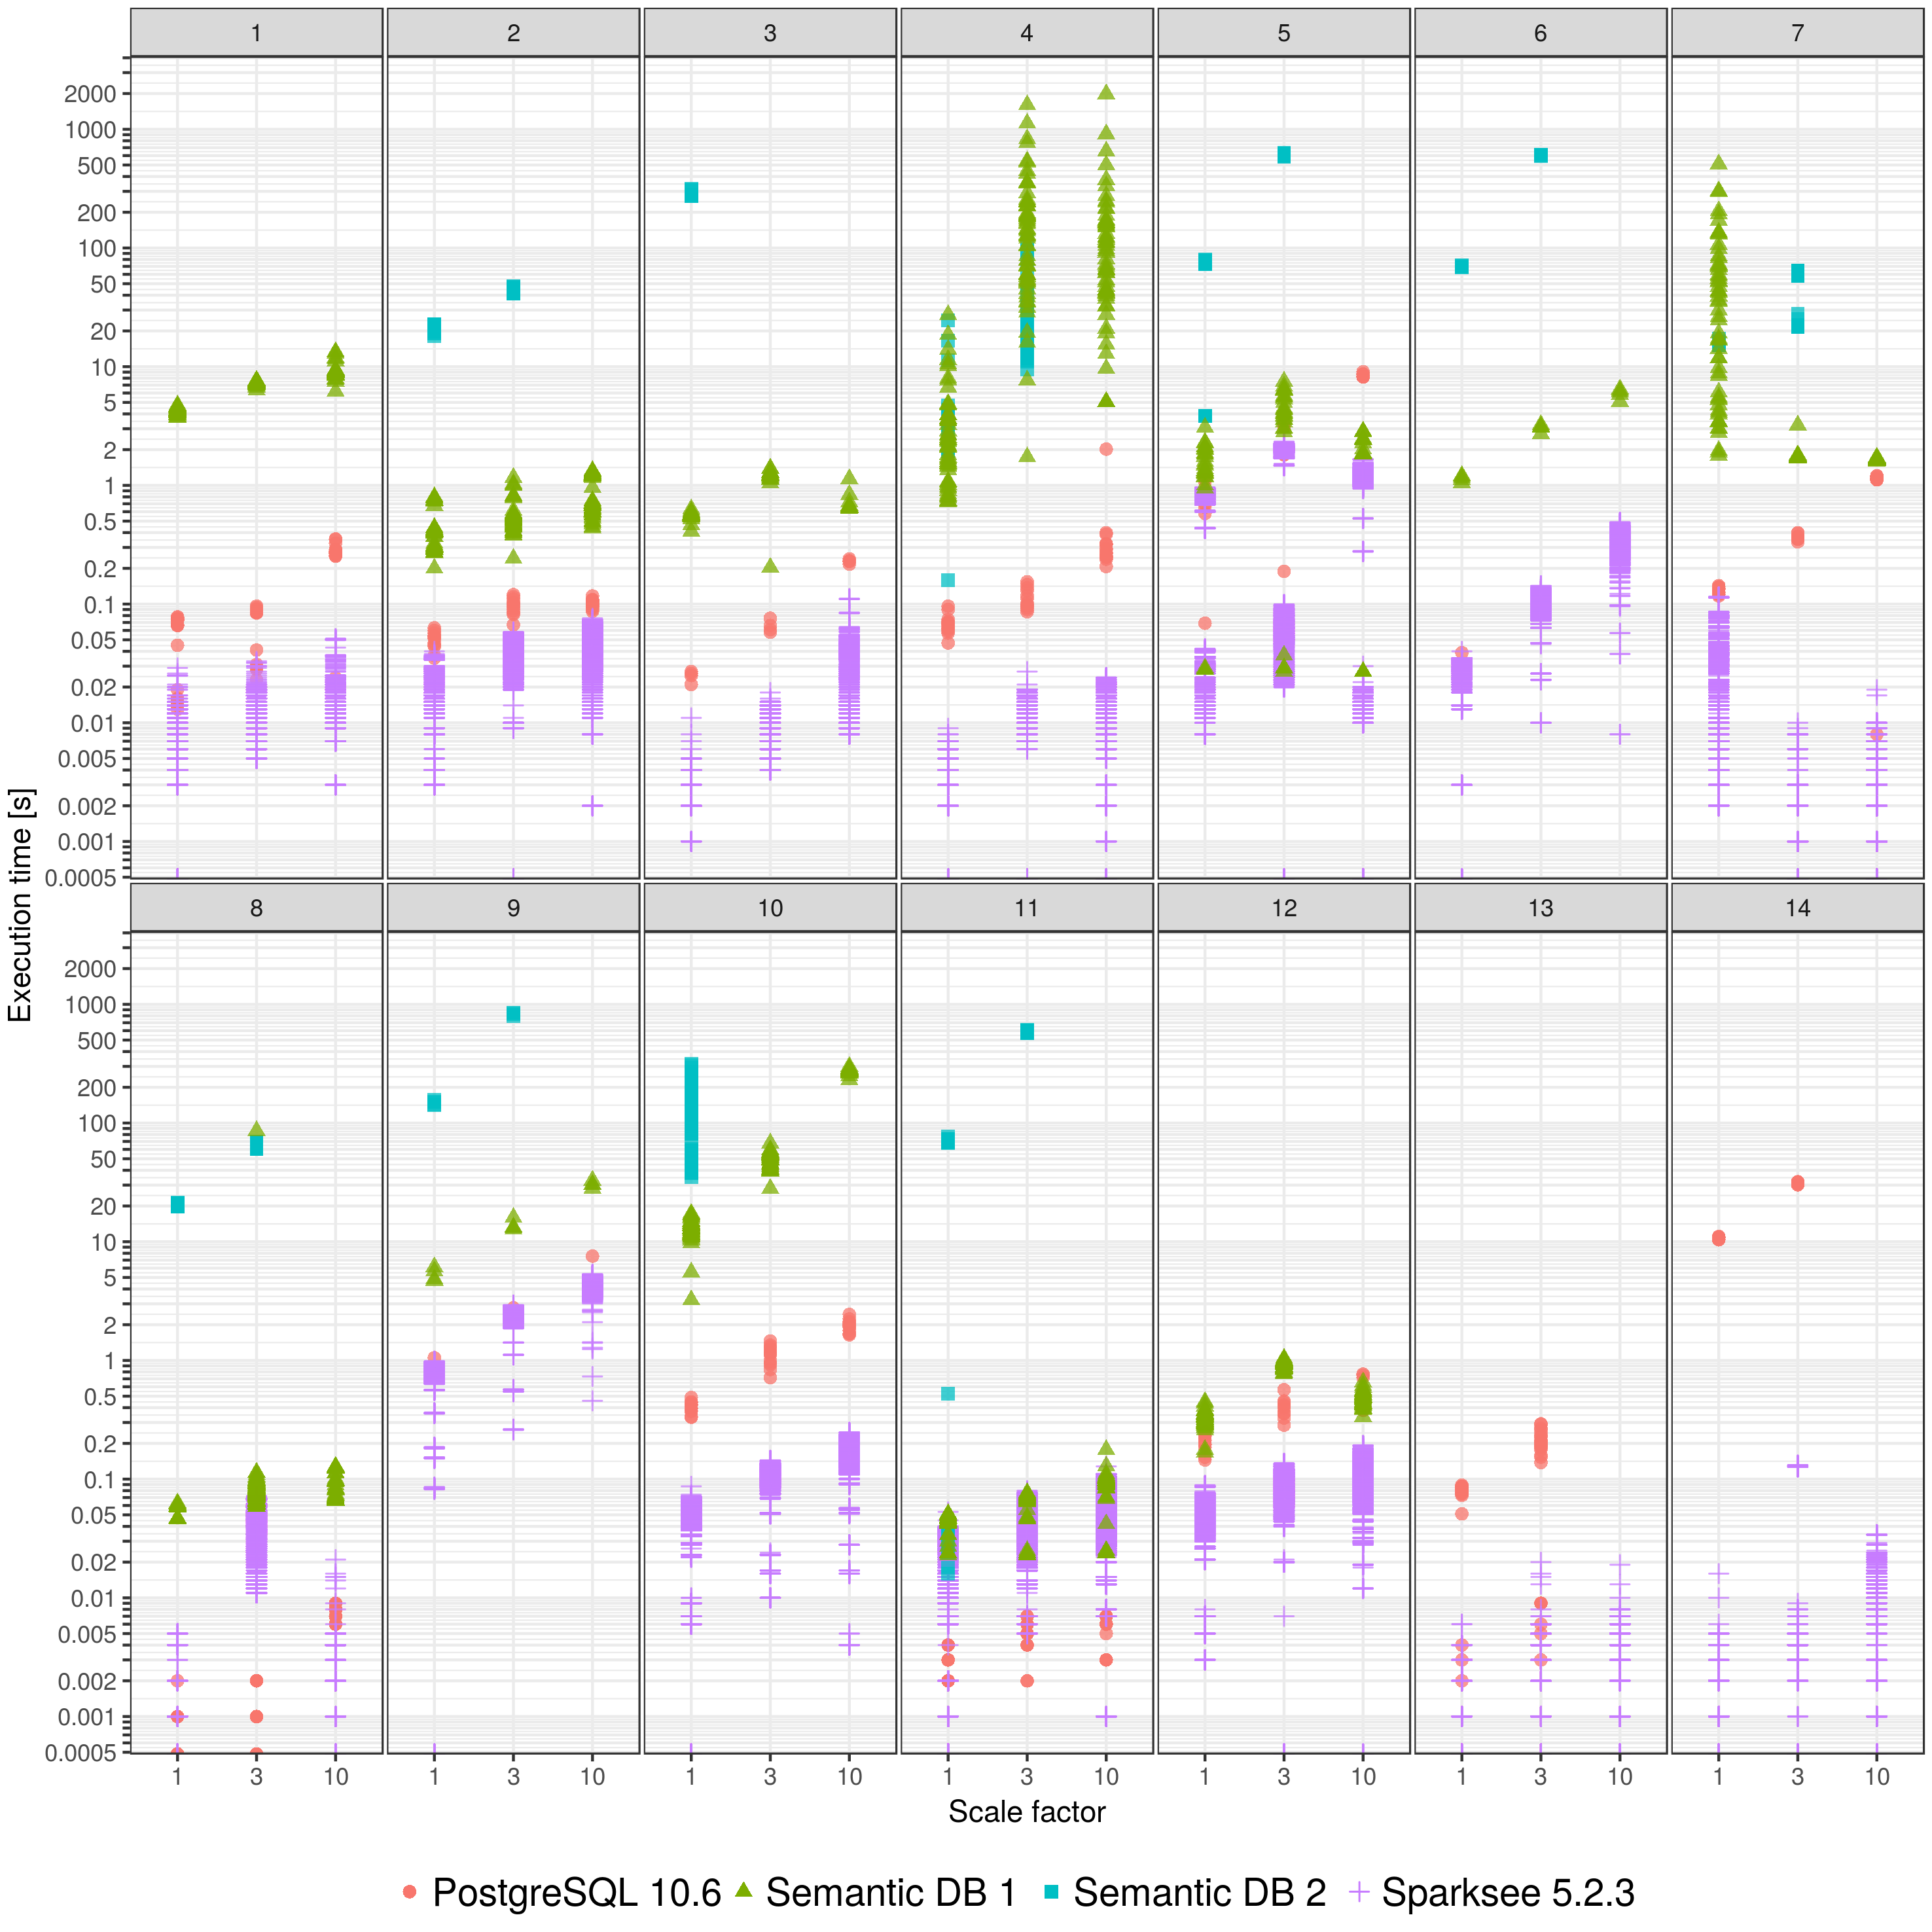
\includegraphics[scale=\plotscale]{results/results-interactive-detailed.png}
	\caption{A lekérdezések részletes mérési eredményei}
	\label{fig:results-interactive-detailed}
\end{figure}

A lekérdezések részletesebb eredményeit ábrázolja \aref{fig:results-interactive-detailed}.~ábra. Megfigyelhető, hogy az eszközök egy adott lekérdezés esetében is nagyságrendekkel eltérő válaszidővel rendelkezhetnek a lekérdezés paramétereitől függően. Kifejezetten látványos az \virtuoso viselkedése a 4-es lekérdezés esetében, ahol a legjobb és a legrosszabb eredmény között több, mint két nagyságrendnyi az eltérés.

Hasonlóan érdemes megvizsgálni a Sparksee viselkedését az 5-ös lekérdezés esetében. A mérési eredmények mindhárom méretű adathalmazon két jól elkülöníthető csoportba sorolhatóak: \textit{(1)} az 1 tizedmásodperc alatti és az \textit{(2)} egy másodperc körüli válaszidők csoportjába. Előbbiekre lehetséges magyarázat lehetne az, hogy a lekérdezés ebben az esetben üres eredményhalmazt ad vissza, de tapasztalataim szerint ez nem igaz.

Az említett jelenségek többségére sajnos hipotéziseket sem tudtam felállítani. Ennek egyik oka, hogy a rendszerek belső működéséről nincs információm, ezért nem tudok következtetni a lehetséges okokra.

\section{Differenciális adatfolyamok teljesítménymérése TTC-vel}

\subsection{Motiváció}

A DAF számítási modell pozitív tulajdonságai miatt (elosztott, nagy teljesítményű, iteratív és inkrementális számítások támogatása) a hatékony INK egyik lehetséges megoldása lehet. A gráfadatbázisokban való felhasználásához azonban fontos tisztában lenni azzal, hogy a gráf alapú adathalmazokon milyen teljesítményt nyújt. Ez a cél tökéletesen illeszkedik a TTC 2018-as versenyfeladatához, ahol a cél az, hogy minél jobb teljesítményű (skálázódás és válaszidő szempontjából is) megoldást készítsünk. Ezért elkészítettem a feladat megoldását a Naiad szoftverkönytár által nyújtott DAF keretrendszerrel, teljesítményét pedig összehasonlítottam a többi megoldás teljesítményével. Így a mérés során az alábbi eszközök teljesítményét hasonlítottam össze:
\begin{itemize}
	\item DAF implementáció a Naiad könyvtár használatával, 1, 2, 4, 6 és 8 szálon történő feldolgozással
	\item NMF alapú inkrementális megoldás
	\item \viatra alapú inkrementális megoldás
	\item Xtend nyelven\footnote{\url{https://www.eclipse.org/xtend/}} manuálisan megvalósított inkrementális megoldás
\end{itemize}
Az Xtend egy Java forráskódra forduló programozási nyelv. Szintaxisa nagyon hasonló a Java nyelvhez, azonban számos szintaktikai édesítőszerrel egészíti ki annak szintaxisát.

\subsection{Mérési elrendezés}\label{sec:naiad-layout}

A méréseket egy számítógépen végeztem el a TTC által nyújtott keretrendszer használatával. A számítógép 6 fizikai processzormagot (Intel Core i7-8700K @ 3.70GHz) és 32 GB memóriát tartalmaz. A háttértár SATA2 interfészen csatolt 512GB-os SSD lemez. Az operációs rendszer 64 bites Windows 10.

A Java környezetből az Oracle Java 8u191-es, a .NET Core 2.2-es és a .NET Framework 4.7.2-es verzióját használtam a mérés során. Az eszközök mérése során a különböző adathalmazokon 3-szor futtattam minden eszközt, az eredményeket aggregáltam az értékek mértani közepét (geometric mean) véve, \cite{DBLP:journals/cacm/FlemingW86} javaslatának megfelelően. Egy futtatás alkalmával a TTC által az adott modellhez tartozó összes (20 darab) frissítést végrehajtottam és a modell betöltése és minden frissítés után lefuttattam a mért lekérdezést. A két lekérdezés mérése szekvenciálisan, átlapolódás nélkül történt történt.

A mérés során használt modelleket egy számmal azonosítjuk. A modellek számozása megegyezik a 2 hatványaival, mivel a legkisebb modellt önkényesen 1-gyel jelölték és a modellek mérete nagyjából duplázódik. A modellek legfontosabb jellemzőit \aref{tab:ttc-modells}.~táblázat mutatja be.
\begin{table}[h]
	\centering
	\begin{tabular}{rrrrr}
		\toprule
		\multicolumn{1}{l}{Modell} & \multicolumn{1}{l}{Felhasználók} & \multicolumn{1}{l}{Bejegyzések}& \multicolumn{1}{l}{Hozzászólások} & \multicolumn{1}{l}{Méret (MB)} \\
		\midrule
		1 & 80 & 554 & 638 & 0.154 \\
		2 & 118 & 889 & 1\,059 & 0.252 \\
		4 & 190 & 1\,845 & 2\,305 & 0.538 \\
		8 & 204 & 2\,270 & 5\,027 & 0.984 \\
		16 & 394 & 5\,518 & 9\,136 & 2.1 \\
		32 & 595 & 10\,929 & 18\,689 & 4.3 \\
		64 & 781 & 18\,083 & 38\,753 & 8.3 \\
		128 & 1\,158 & 37\,228 & 75\,605 & 18 \\
		256 & 1\,678 & 74\,668 & 145\,821 & 34 \\
		512 & 2\,606 & 167\,299 & 267\,160 & 68 \\
		1\,024 & 3\,699 & 314\,510 & 526\,006 & 136 \\
		\bottomrule
	\end{tabular}
	\caption{Az egyes modellekben szereplő modellelemek darabszáma (db) és a kezdeti modell mérete MB-ban}
	\label{tab:ttc-modells}
\end{table}

A \viatra és Xtend alapú megoldásokat nem mértem a nagyobb adathalmazokon, mivel a teljesítménymérés túl hosszú ideig tartott volna.

\subsubsection{Eredmények értékelése}

Az eredmények értékelésénél fontos kiemelni, hogy a mért lekérdezések validáltak, de nem auditáltak (azaz az eszközök fejlesztői által nem vizsgáltak, így nem garantált, hogy optimális teljesítményt nyújtanak).

\begin{figure}[ht!]
	\centering
	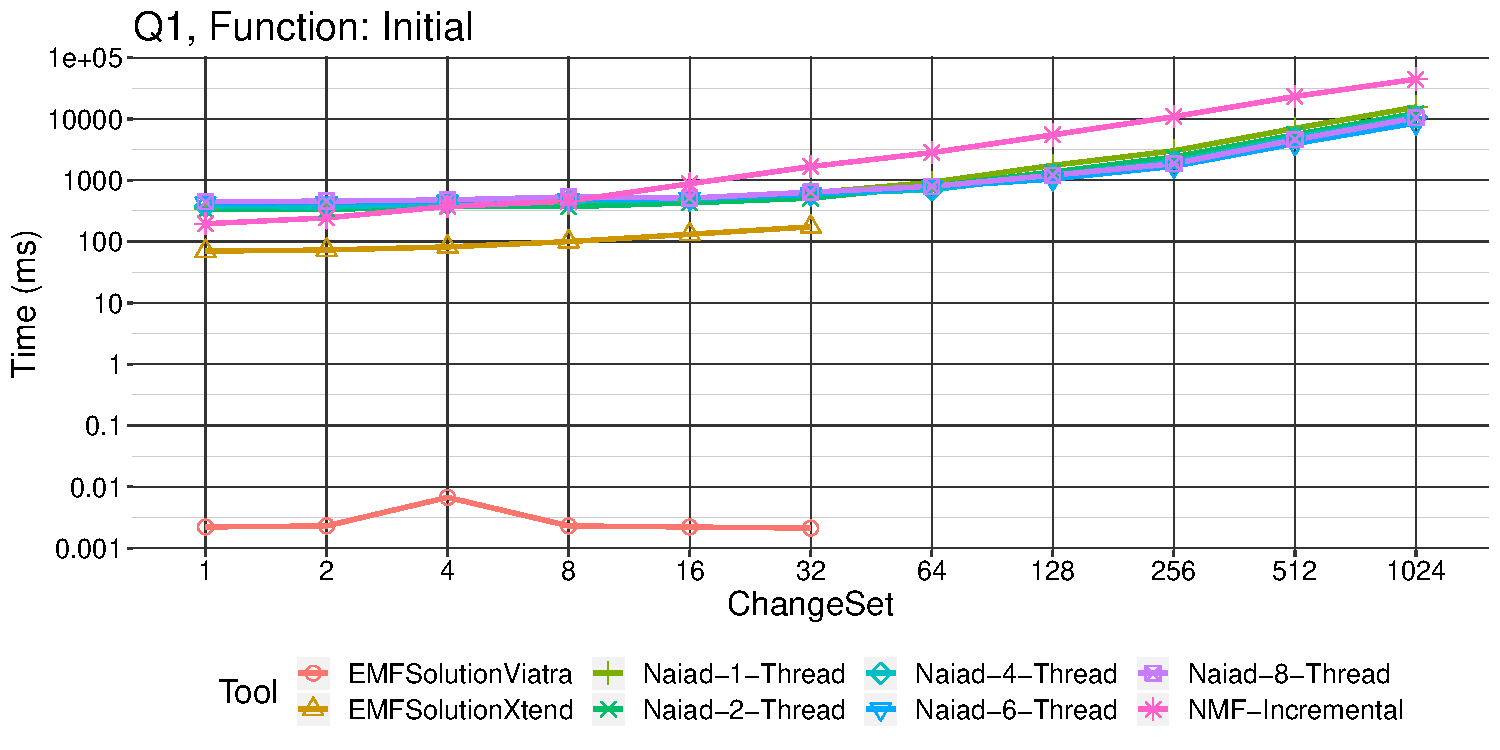
\includegraphics[width=150mm, keepaspectratio]{q1_initial}
	\caption{A Q1 lekérdezés első kiértékeléseinek válaszidői}
	\label{fig:q1_initial}
\end{figure}
\begin{figure}[ht!]
	\centering
	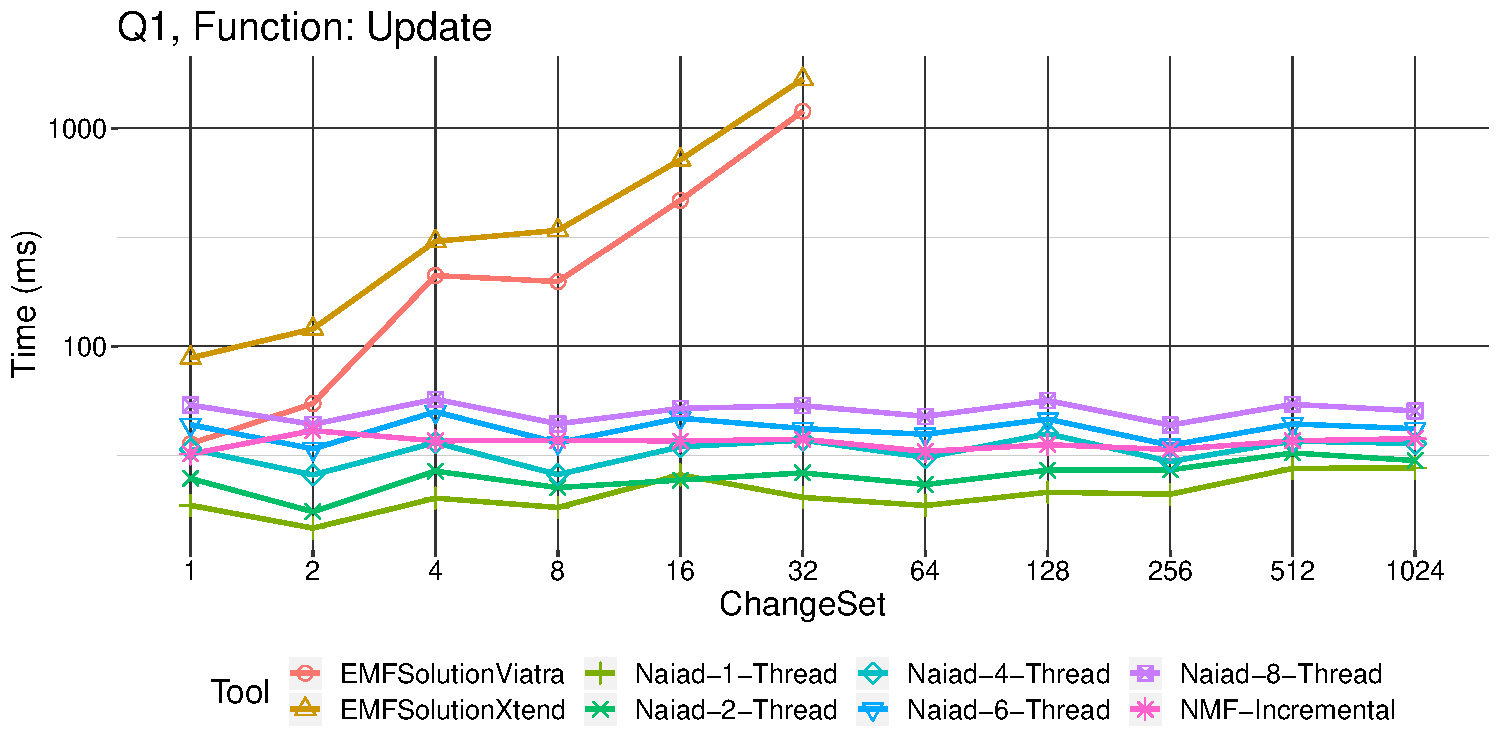
\includegraphics[width=150mm, keepaspectratio]{q1_update}
	\caption{A Q1 lekérdezés frissítések utáni kiértékeléseinek válaszidői}
	\label{fig:q1_update}
\end{figure}

\begin{table}[ht!]
	\centering
	\begin{tabular}{rrrrrrr}
		\toprule
		\multicolumn{1}{l}{Modell} & \multicolumn{1}{l}{Naiad-1} & \multicolumn{1}{l}{Naiad-2}& \multicolumn{1}{l}{Naiad-4} & \multicolumn{1}{l}{Naiad-6} & \multicolumn{1}{l}{Naiad-8}& \multicolumn{1}{l}{NMF} \\
		\midrule
		1 & 68 & 93 & 141 & 194 & 241 & 48 \\
		2 & 70 & 101 & 152 & 208 & 251 & 54 \\
		4 & 74 & 107 & 166 & 216 & 269 & 70 \\
		8 & 83 & 113 & 176 & 233 & 287 & 84 \\
		16 & 96 & 128 & 190 & 254 & 316 & 155 \\
		32 & 113 & 147 & 209 & 274 & 334 & 274 \\
		64 & 151 & 189 & 255 & 316 & 385 & 445 \\
		128 & 221 & 257 & 324 & 395 & 454 & 853 \\
		256 & 399 & 398 & 471 & 528 & 602 & 1\,408 \\
		512 & 658 & 668 & 729 & 815 & 865 & 3\,346 \\
		1\,024 & 1\,308 & 1\,285 & 1\,300 & 1\,351 & 1\,418 & 6\,424 \\
		\bottomrule
	\end{tabular}
	\caption{A Q1 lekérdezés utolsó kiértékelése utáni memóriahasználat a különböző méretű modellek és eszközök esetében MB-ban}
	\label{tab:q1-memory}
\end{table}

\paragraph{Q1 lekérdezés}

\Aref{fig:q1_initial}.~ábra mutatja a Q1 lekérdezés első kiértékeléseinek válaszidejét a modell méretének függvényében. A legszembetűnőbb eredmény a \viatra rendkívül alacsony, a többi eszköz válaszidejénél nagyjából 4 nagyságrenddel kisebb válaszideje. Ezt az okozza, hogy a \viatra már a betöltés során elkezdi a kiértékelést, és az első lekérdezésnél valószínűsíthetően már rendelkezésre álló eredményeket adja vissza. A többi eszköz közül az Xtend-es megoldás valamivel gyorsabb az Naiad és NMF alapú megoldásoknál. \Aref{fig:q1_update}.~ábrán azonban jól látszik, hogy a \viatra és az Xtend alapú megoldás is jelentősen rosszabbul teljesít, mint a Naiad és NMF alapú megoldások. Jól látható, hogy a Naiad alapú megoldások esetében a válaszidő arányos a feldolgozásra használt szálak számával. Ennek több magyarázata is lehet. Egyik lehetséges magyarázat az, hogy a számítás olyan rövid ideig tart (<100ms), hogy a többszálú feldolgozás akkora plusz komplexitást (overheadet) jelent, hogy ekkora méretű modellek esetében egyszerűen nem éri meg. Egy másik lehetséges magyarázat az, hogy egyszerűen rosszul működik a számítás elosztásáért felelős logika. Ennek eldöntéséhez nagyobb modellekre lenne szükség, ahol a számítások ideje több nagyságrenddel több időt vesz igénybe.

A Naiad teljesítményéről egyébként elmondható, hogy a vizsgált modellek esetében jól skálázódik az NMF alapú megoldással együtt, gyakorlatilag a legkisebb és legnagyobb modellen is azonos válaszidővel rendelkeznek. Érdemes megfigyelni \aref{tab:q1-memory}.~táblázaton, hogy a Naiad alapú megoldások az NMF alapú megoldáshoz képest a kisebb modellek esetén több memóriát használnak, azonban ez nagyjából a 32-es modell környékén megváltozik. A legnagyobb modell esetén az NMF alapú megoldás nagyjából ötször több memóriát használ mint a Naiad alapú megoldások. Ahogy \aref{sec:naiad-layout}.~fejezetben már kitértem rá, a \viatra és az Xtend alapú megoldások nagyjából lineárisan skálázódnak a modell méretéhez viszonyítva.

\begin{figure}[htb]
	\centering
	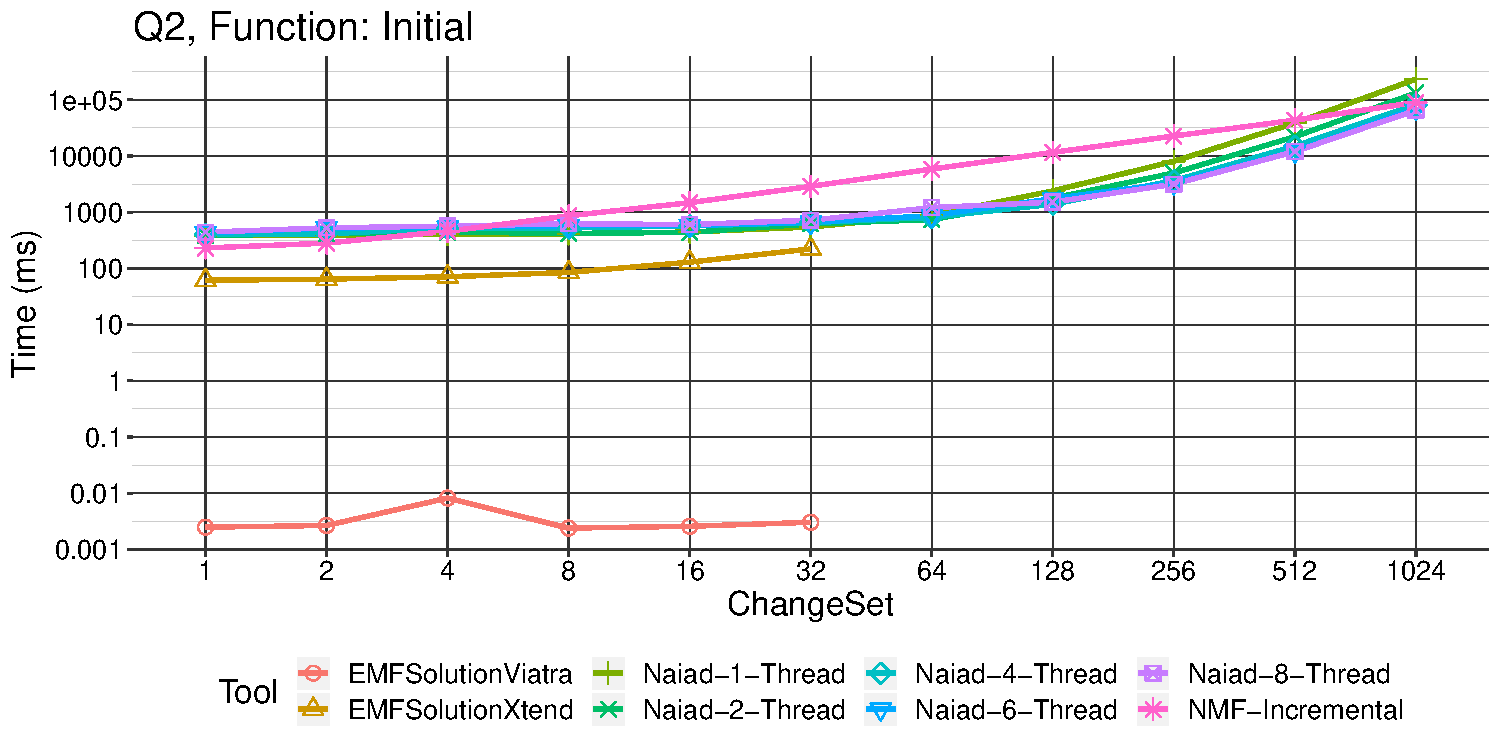
\includegraphics[width=150mm, keepaspectratio]{q2_initial}
	\caption{A Q2 lekérdezés első kiértékeléseinek válaszidői}
	\label{fig:q2_initial}
\end{figure}

\begin{figure}[htb]
	\centering
	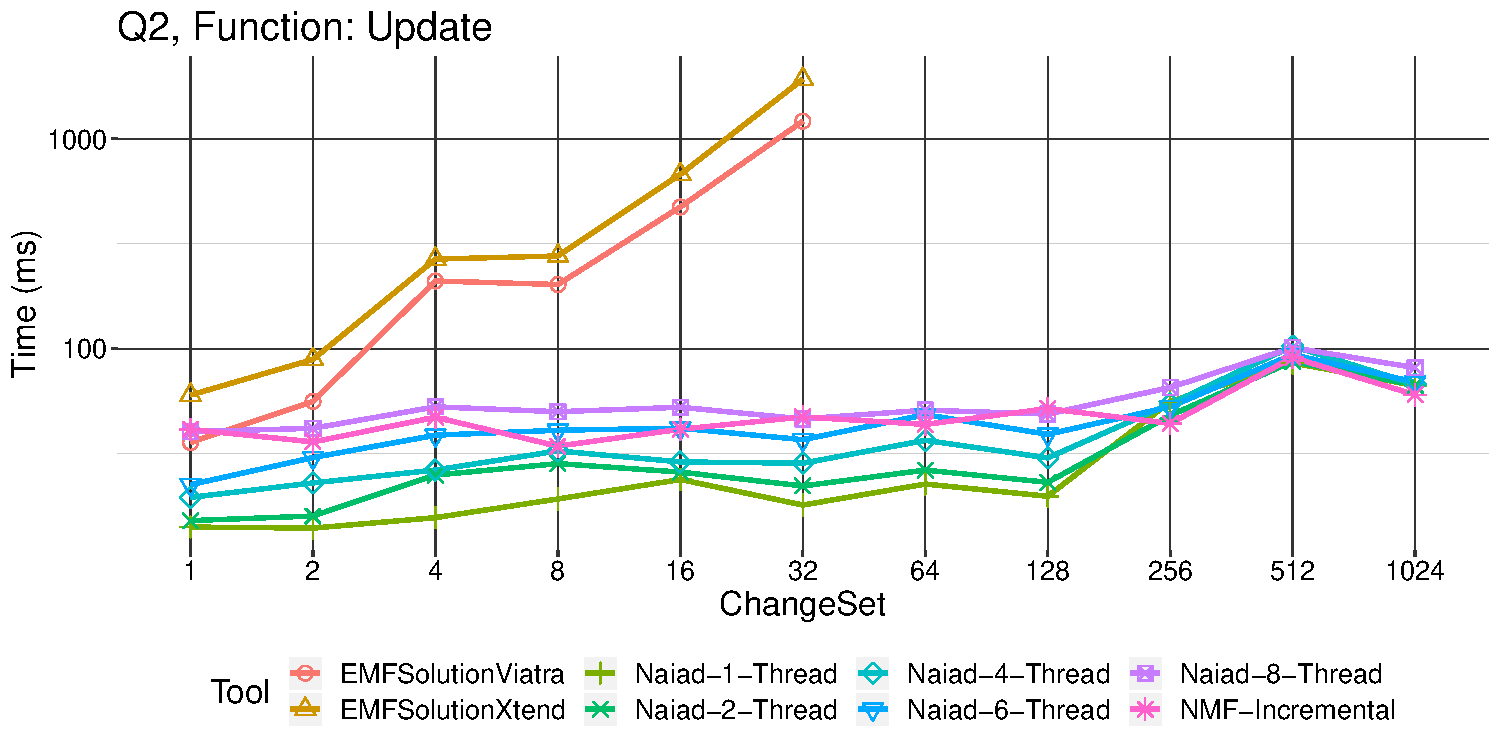
\includegraphics[width=150mm, keepaspectratio]{q2_update}
	\caption{A Q2 lekérdezés frissítések utáni kiértékeléseinek válaszidői}
	\label{fig:q2_update}
\end{figure}

\begin{table}[htb]
	\centering
	\begin{tabular}{rrrrrrr}
		\toprule
		\multicolumn{1}{l}{Modell} & \multicolumn{1}{l}{Naiad-1} & \multicolumn{1}{l}{Naiad-2}& \multicolumn{1}{l}{Naiad-4} & \multicolumn{1}{l}{Naiad-6} & \multicolumn{1}{l}{Naiad-8}& \multicolumn{1}{l}{NMF} \\
		\midrule
		1 & 60 & 71 & 88 & 114 & 123 & 47 \\
		2 & 77 & 113 & 140 & 197 & 208 & 55 \\
		4 & 84 & 127 & 186 & 252 & 300 & 74 \\
		8 & 95 & 137 & 210 & 290 & 351 & 120 \\
		16 & 107 & 155 & 243 & 335 & 414 & 199 \\
		32 & 124 & 181 & 275 & 370 & 464 & 344 \\
		64 & 168 & 224 & 330 & 444 & 555 & 681 \\
		128 & 251 & 318 & 444 & 555 & 679 & 1301 \\
		256 & 433 & 527 & 639 & 777 & 905 & 2537 \\
		512 & 929 & 997 & 1\,148 & 1\,251 & 1\,410 & 4\,882 \\
		1\,024 & 2\,281 & 2\,398 & 2\,546 & 2\,679 & 2\,836 & 9\,864 \\
		\bottomrule
	\end{tabular}
	\caption{A Q2 lekérdezés utolsó kiértékelése utáni memóriahasználat a különböző méretű modellek és eszközök esetében MB-ban}
	\label{tab:q2-memory}
\end{table}

\paragraph{Q2 lekérdezés}

\Aref{fig:q2_initial}.~ábrán látható a Q2 lekérdezés első kiértékeléseinek válaszidői a modell méretének függvényében. Az eredmények trendje nagyjából megegyezik a Q1 lekérdezés eredményével, azonban fontos észrevenni, hogy a legnagyobb modellen már egy nagyságrenddel több időt vett igénybe az első kiértékelés a Naiad és az NMF alapú megoldások esetében is. A \viatra kiugróan alacsony válaszidejének oka a Q1 lekérdezésnél leírt betöltési mechanizmus. \Aref{fig:q2_update}.~ábrán pedig a frissítések utáni kiértékelések válaszidejét tekinthetjük meg, valamint \aref{tab:q2-memory}.~táblázatban a használt memória mennyiségét. A válaszidőkről és a memóriahasználatról is nagyjából hasonló megállapítások mondhatóak el, mint a Q1 lekérdezés esetében.

Az egyetlen különböző és egyben érdekes dolog, ami a Naiad és az NMF megoldásra is jellemző a 256-os megoldástól kezdve: a válaszidők elkezdenek konvergálni, azonban nem kezd el jelentősen nőni a válaszidő. Mivel mindkét megoldás C\texttt{\#} alapú, ezért egy lehetséges magyarázat az, hogy a \emph{just-in-time} fordító (JIT) úgy értékeli a program futtatását, hogy érdemes az egyik gyakran használt kódrészletét alaposabban optimalizálni, ezért azt a kódrészletet újrafordítja, ami összemérhető nagyságrendű az egyébként nagyon alacsony válaszidővel.

% !TeX spellcheck = hu_HU
% !TeX encoding = UTF-8
\chapter{Kapcsolódó munkák}\label{sec:kapcsolodo}

\section{Gráf adathalmazok lekérdezése}
\paragraph{Cypher}
A Cypher nyelvhez elérhető a \emph{Cypher for Apache Spark}\footnote{\url{https://github.com/opencypher/cypher-for-apache-spark}} projekt, ami a népszerű Spark keretrendszeren futtatható programokra képez le openCypher lekérdezéseket. A Cypher for Apache Spark projekt megoldása a Spark adatfolyam-orientált (streaming) programozási modellje miatt nem alkalmas módosítás és törlés műveletek kezelésére.

\paragraph{G-CORE}
A G-CORE~\cite{DBLP:conf/sigmod/AnglesABBFGLPPS18} az LDBC Graph Query Language munkacsoportjának és több cég közreműködésével tervezett lekérdezési nyelv a tárolt utakkal rendelkező tulajdonsággráfokhoz (path property graph). Ebben az adatmodellben az éleken túl lehetőség van utak és azok tulajdonságainak tárolására is. A G-CORE lehetőséget nyújt az utak és tulajdonságaik lekérdezésére, módosítására. A G-CORE tervezésére befolyással volt a Cypher nyelv, így a szemantikai hasonlóságok mellett sok konstrukció azonos szintaxissal definiálható.

\paragraph{Datalog}
A Datalog egy deklaratív programozási nyelv, amely szintaktikailag a Prolog nyelv részhalmaza. Datalogban sor- és oszlopkalkulushoz hasonló lekérdezéseket lehet megfogalmazni. Számos kiterjesztése létezik, amelyeket különböző adatbázis-kezelőkben használnak, például LogiQL nevű kiterjesztését a LogicBox adatbázis-kezelőben~\cite{DBLP:conf/sigmod/ArefCGKOPVW15}.

\paragraph{VIATRA Query Language}

A gráfmintaillesztést széles körben használják a modellvezérelt technológiákban, például a \viatra keretrendszerben~\cite{DBLP:journals/sosym/VarroBHHRU16}. A keretrendszer saját lekérdezőnyelve egy Dataloghoz hasonló nyelv, a \vql (VQL), amely támogatja a gráfminták komponálását, a rekurzív minták megfogalmazását és az aggregációt. A \viatra keretrendszer a Rete algoritmust használja a gráfmodellek hatékony ellenőrzésre és transzformációjához. Az \iqd egy elosztott inkrementális gráflekérdező~\cite{DBLP:conf/models/SzarnyasIRHBV14}, amely lekérdezőnyelve a VQL-en alapul és RDF gráfok lekérdezését teszi lehetővé.

A \viatra egy korábbi verziójában készült egy prototípus alkalmazás~\cite{DBLP:conf/gg/BergmannHH12}, ami inkrementális gráftranszformációt végez relációs adatbázisokon. A prototípus  gráfmintákból SQL lekérdezéseket készít a kezdeti illeszkedési halmazok meghatározásához. Egy mintát egy több illesztést tartalmazó, lapos SQL lekérdezéssé képez le. Ezután az illeszkedési halmazokat az adatbázis triggereinek (adott esemény hatására lefutó SQL kifejezések, például sorok beszúrása, törlése vagy módosítása) használatával tartja karban.



\section{Teljesítménymérési keretrendszerek gráflekérdezésekre}

A dolgozat készítése során több teljesítménymérési keretrendszert tanulmányoztam, amelyek lehetővé teszik gráf információs rendszerekben futtatott lekérdezések teljesítményének vizsgálatát. Az általam fontosnak vélt keretrendszerek legmeghatározóbb tulajdonságait mutatom be ebben a fejezetben.

\paragraph{LDBC Semantic Publishing Benchmark}
Az LDBC egy másik teljesítményérési keretrendszere a Semantic Publishing Benchmark~\cite{DBLP:conf/semweb/KotsevMPEFK16} (SPB), amely a British Broadcasting Corporation\footnote{\url{http://www.bbc.com/}} (BBC)  Dynamic Semantic Publishing rendszeréhez hasonló RDF adathalmazt használ. Az adathalmazban különböző kreatív munkák (cikkek, fényképek és videók) érhetőek el különböző szempontok szerint csoportosítva. A teljesítménymérés során párhuzamosan futnak szerkesztői módosítások, beszúrások és a felhasználói lekérdezések az állandó terhelést szimulálva. A mérés során az LDBC SNB-hez hasonlóan az adatbázis-kezelők hatékonyságát leíró jellemzőket rögzít.

Azon túl, hogy csak RDF adathalmaz generálására alkalmas, az LDBC SPB a teljesítménymérés során olyan csak RDF-ben elérhető funkciókat használ, mint a következtetés (\textit{inferencing}), azaz a meglévő kapcsolatok és előre definiált szabályok alapján új kapcsolatok létrehozása. A keretrendszer ezen tulajdonsága miatt nem alkalmas tulajdonsággráf alapú vagy relációs adatbázis-kezelők teljesítménymérésére.

\paragraph{Train Benchmark}
A Train Benchmark~\cite{DBLP:journals/sosym/SzarnyasIRV18} a modellvezérelt technológiák által inspirált teljesítménymérési keretrendszer, amely adatmodellje a vasúthálózat és a hozzá kapcsolódó érzékelő és biztosító berendezések hálózatát tartalmazza. Többféle terhelési profilt definiál, több adatmodellt és lekérdezőnyelvet is támogat, köztük az ebben a dolgozatban használtakat is. Az LDBC SNB keretrendszernél azonban kevesebb nyelvi elemet fed le, például nem teszi lehetővé aggregációk, útvonal-kifejezések vagy éleken definiált tulajdonságok teljesítménymérését.

\section{Illesztések optimalizációja gráfadatbázis-kezelőkben}

A relációs adatbázis kezelők elterjedésének köszönhetően az elmúlt évtizedekben egyre hatékonyabb illesztési algoritmusokat dolgoztak ki. A lekérdezések végrehajtási tervének optimalizálása a végrehajtási terv elemei közötti egymásra épülésének (kb. végrehajtási sorrend, amolyan termelő-fogyasztó viszony) -- a szelekciós tényező becsült értékén alapuló -- ekvivalens átalakításain alapszik. A szelekciós tényező egy illesztés esetén az eredményként előálló reláció sorainak számának aránya az alaprelációk Descartes-szorzatának sorainak számához viszonyítva. Formálisan $ s = \frac{|R_1 \joinop R_2|}{|R_1 \times R_2|} $, ahol $s$ a szelekciós tényező, $R_1$ és $R_2$ pedig az illesztés két alaprelációja. Az illesztési sorrend nagyon fontos a hagyományos relációs lekérdezésekben, így egy jó illesztési sorrenddel sokat lehet nyerni, a hiányában bukni. Annak ellenére, hogy a relációs adatbázis kezelőkben az ezen alapuló algoritmusok és módszerek hatékonynak bizonyultak, a gráfadatbázis kezelők tekintetében sok esetben nem bizonyultak megfelelőnek. A problémát a gráfos lekérdezések tulajdonságai, a tipikusan használt gráfminták okozzák, amelyek általában nincsenek jelen a relációs lekérdezésekben, pl. a körkörös gráfminták, vagy az adatok szokatlan eloszlása. 

\begin{figure}[ht]
	\centering
	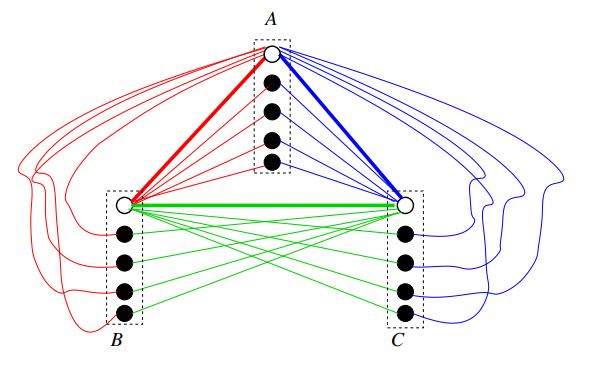
\includegraphics[width=120mm, keepaspectratio]{king}
	\caption{{$\circ$} királyok, {$\bullet$} alattvalók~\cite{DBLP:journals/sigmod/NgoRR13}}
	\label{fig:king}
\end{figure}

\subsection{Körkörös lekérdezés}

A relációs adatbázissal szemben a gráfadatbázisok esetében gyakoriak a köröket tartalmazó lekérdezések. Mivel a relációs adatbázis-kezelőkben a bináris (két alaprelációt tartalmazó) illesztések beváltak, így számos gráfadatbázis is bináris illesztéseket használ az illesztések elvégzésére, köztük a tanszéken fejlesztett ingraph~\cite{DBLP:conf/sdl/MartonSB17} inkrementális gráfadatbázis-kezelő rendszer is. A bináris illesztések rossz teljesítményét \aref{fig:king}.~ábrán látható gráfon mutatom be:
tegyük fel, hogy a három, szaggatott vonallal jelölt királyságban egyik király (üres körök) sem ismeri a saját alattvalóit (teli körök), de minden más királyság összes alattvalóját és a királyukat is ismeri. Ha ebben a gráfban a pontosan 3 darab, páronként különböző színű élt tartalmazó köröket keressük, akkor bináris illesztéseket használva \aref{fig:king_plan}.~ábrán látható végrehajtási tervek egyikét kell végrehajtanunk. Az ábrán \textcolor{red}{\textit{R}}, \textcolor{green}{\textit{S}} és
\textcolor{fullblue}{\textit{T}} az azonos színű élhalmazokat jelentik. Ekkor a második (a végrehajtási terveben legfelső) illesztés alaprelációinak 25 (az első illesztés eredménye) és 9 (a harmadik színű élek) darab sora lesz, az illesztés eredménye pedig 13 darab ($3 \times 4$ darab pontosan kettő királyt tartalmazó kör és 1 darab mindhárom királyt tartalmazó kör) sorból fog állni. Ezek alapján a szelekciós tényező $s = \frac{13}{25 \times 9} \approx 0.058$. Az alacsony szelekciós tényező miatt
ebben az esetben a bináris illesztésnél létezik hatékonyabb módszer is~\cite{DBLP:journals/sigmod/NgoRR13}, a WCOJ (worst-case optimal join) algoritmusok~\cite{DBLP:journals/jacm/NgoPRR18}. Ezek az algoritmusok egyszerre nem kettő, hanem több, akár tetszőleges számú reláció illesztését végzik el egyszerre. Egy ilyen algoritmus a Leapfrog Triejoin~\cite{DBLP:conf/icdt/Veldhuizen14}, ami olyan attribútumok illesztését képes hatékonyan elvégezni, amelyeken értelmezett a rendezés művelet.
A WCOJ algoritmusok kifejezetten az ilyen lekérdezések hatékony végrehajtását segítik. Véleményem szerint \emph{az ingraph teljesítményét jelentősen növelné}, ha a bináris illesztések mellett WCOJ algoritmusokat is megvalósítana.

\begin{figure}[ht]
	\centering
	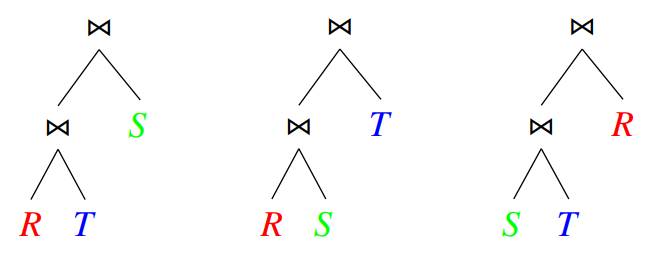
\includegraphics[width=60mm, keepaspectratio]{king_plan}
	\caption{A lehetséges végrehajtási tervek bináris illesztések esetén~\cite{DBLP:journals/sigmod/NgoRR13}}
	\label{fig:king_plan}
\end{figure}

\subsection{Eredmények számosságának becslése}
Mivel az illesztések szelekciós tényezőjének pontos kiszámítása túl költséges művelet, ezért az adatbázis-kezelő rendszerekben gyakran használnak különböző becsléseket (\emph{cardinality estimation}) a szelekciós tényező meghatározására, hogy a lekérdezések végrehajtási tervét ennek figyelembevételével készítsék el.
Az ilyen becslések két nagy csoportba sorolhatóak~\cite{DBLP:journals/vldb/LeisRGMBKN18}:
az \textit{(1)} aggregált adatokon (hisztogramokon) alapuló és
a \textit{(2)} mintavételezésen alapuló becslések.

Az \textit{(1)} esetben az adatbázis-kezelő rendszereknek fel kell építeniük és karban kell tartaniuk az alaprelációkról a szükséges statisztikákat. Ahhoz, hogy az aggregált adatokból megfelelő pontossággal lehessen megbecsülni a szelekciós tényezőt, sok esetben pontosan ismerni kell az adatok struktúráját, esetleg részletesebb statisztikákat kell tárolni és frissíteni. Extrém nagy adathalmazok esetén az is előfordulhat, hogy már a statisztikákat is becslésekkel állítják elő, így növelve a becslés pontatlanságát.

A \textit{(2)} esetben a bemeneti relációk néhány rekordját kiválasztjuk, majd ezek illesztése után az eredeti relációk illesztésének szelekciós tényezőjét becsüljük a kiválasztott elemek szelekciós tényezőjével. A mintavételezésen alapuló eljárások nem követelik meg az adatbázisra vonatkozó statisztikák tárolását és karbantartását, valamint korrelált és nem egységes adatok esetében robusztusak~\cite{DBLP:journals/jcss/HaasNSS96}. Továbbá a mintavétel alapú eljárások lehetővé teszik a becslési hibák értékelését és ellenőrzését. A mintavételezés történhet több lépésben is: minden lépésben kiválasztunk $ n \ge 1$ rekordot mindkét relációból, ezeket illesztjük majd a mintavételezési lépések után azok eredményeit kombináljuk és következtetünk az eredeti illesztés szelekciós tényezőjére. Az egyes lépések után a mintavételezett rekordokat a későbbi lépésekben felhasználhatjuk, vagy akár el is dobhatjuk. A mintavételezési lépések száma lehet egy előre rögzített szám, vagy a mintavételezés folytatódhat addig, amíg egy bizonyos valószínűséget el nem ér a becslés pontossága (azaz amíg nem vagyunk elég biztosak a becslés helyességében).

A gráfadatbázisok egy fontos tulajdonsága, hogy a csúcsok fokszámeloszlása erősen eltolt (skewed).
Míg relációs adathalmazok gyakran normál vagy teljesen véletlenszerű eloszlást követnek,
addig előbbiek általában a hatványtörvény-eloszlást (power law distribution) követik~\cite{Barabasi:2003:ITS}.
A hatványtörvény-eloszlás egy olyan valószínűség-eloszlás, melynek sűrűségfüggvénye
$$ P(X>x)\sim L(x)x^{-(\alpha +1)} $$
alakú, ahol $\alpha > 0$, és $L(x)$ egy lassan változó függvény, amire minden pozitív $r$ esetében igaz, hogy:
$$\lim _{x\rightarrow \infty } \frac{ L(r \cdot x) }{ L(x) } = 1.$$
Egy példa hatványtörvény-eloszlás \aref{fig:powerlaw}.~ábrán\footnote{Forrás: Wikipédia, \url{https://en.wikipedia.org/wiki/Power_law}} látható.
\begin{figure}[ht]
	\centering
	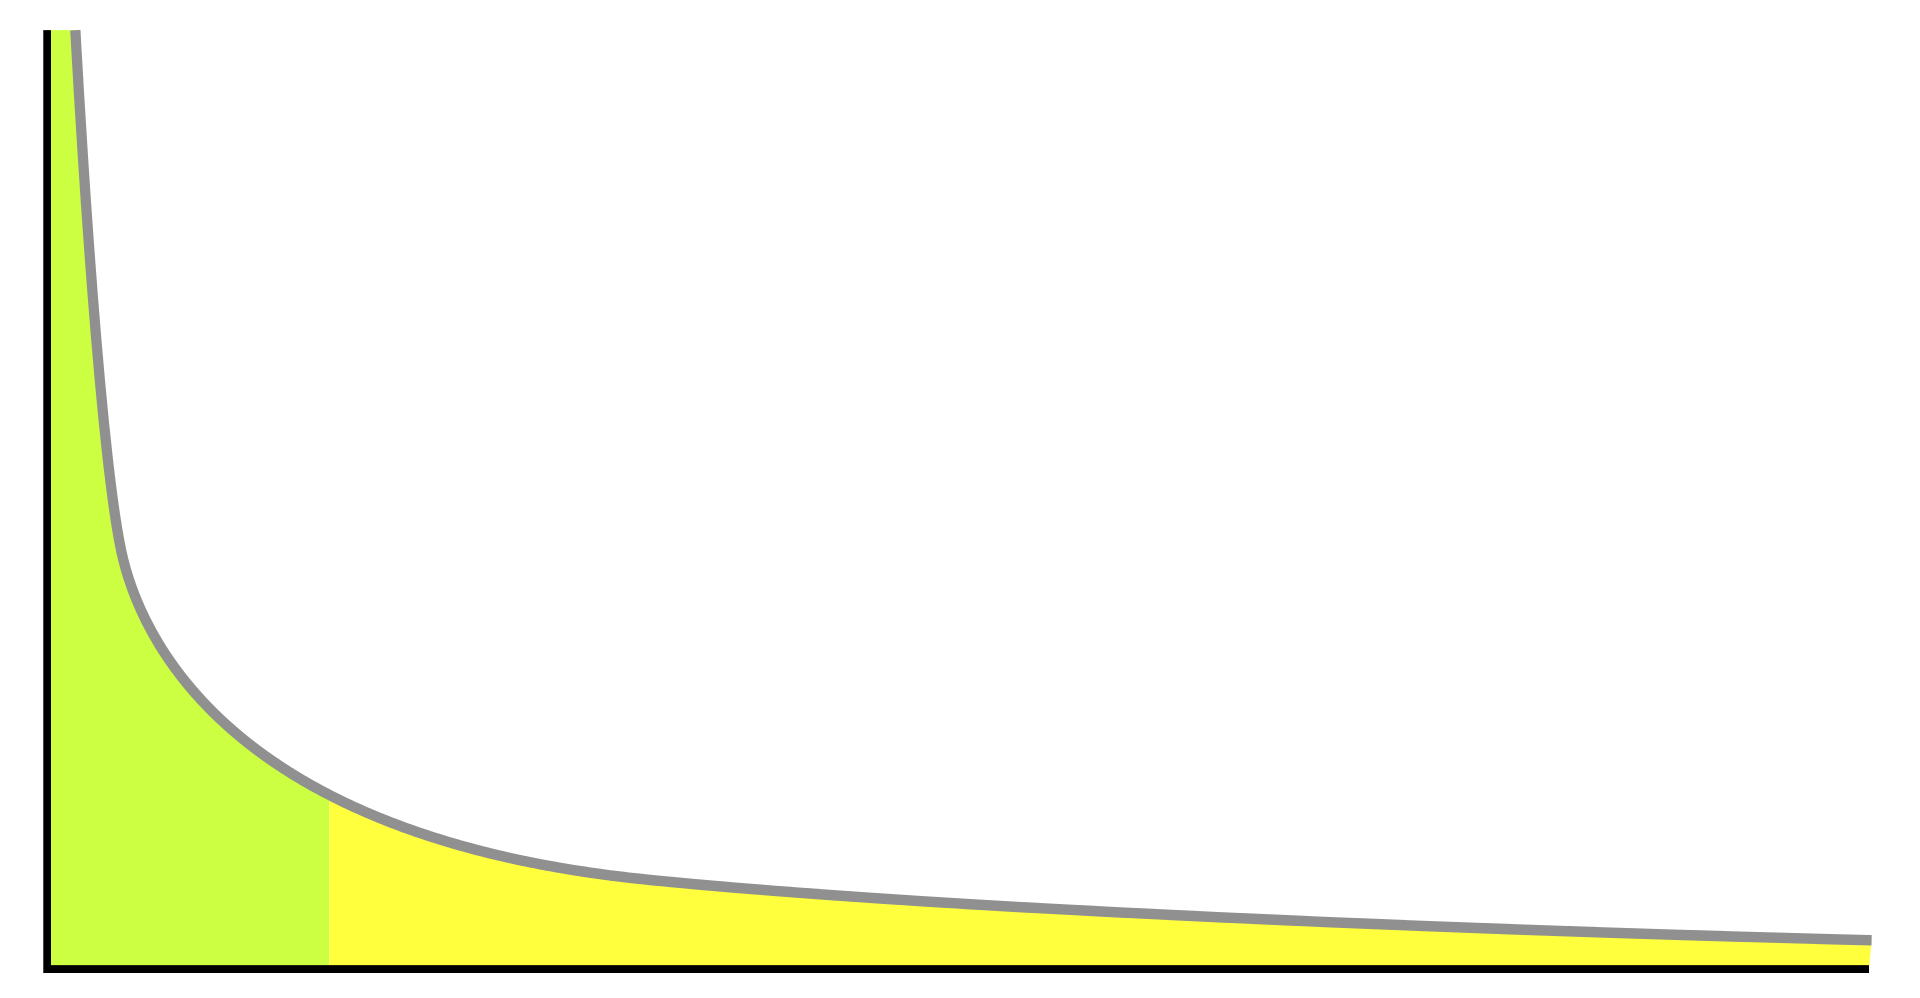
\includegraphics[width=90mm, keepaspectratio]{powerlaw}
	\caption[Egy példa határtörvény-eloszlás]{Egy példa határtörvény-eloszlás, sárgával van jelölve az eloszlás farka (\emph{tail}), zölddel pedig a domináns fej (\emph{head}) rész -- a jól ismert 80-20 szabályhoz hasonlóan.}
	\label{fig:powerlaw}
\end{figure}
\paragraph{Javaslat az ingraph rendszer továbbfejlesztésére}
Ezen ismeretek alapján az ingraph rendszerben szerintem a mintavételezésen alapuló becslési módszert érdemes implementálni, figyelembe véve az \textit{end-biased}~\cite{DBLP:conf/icde/EstanN06} módszert. Ennek a módszernek a lényege, hogy az egyes elemek gyakoriságát nyilvántartja, és az alapján választja ki a mintavételezés során az elemeket. Egy adott $T$ gyakoriság felett minden elemet belevesz a mintába, alatta pedig a gyakoriságával arányos valószínűséggel választja bele a mintába az egyes elemeket. Ez a módszer biztosíthatja, hogy a legmeghatározóbb (leggyakoribb) elemek kiválasztásra kerüljenek, azonban a kevésbé gyakori, azonban összességében az adathalmaz jelentős részét alkotó -- \aref{fig:powerlaw}.~ábrán sárgával jelölt -- elemek közül is megfelelő mennyiségű a mintába kerüljön, így növelve a becslés pontosságát. A módszer lehetőséget biztosít arra, hogy megfelelő hash függvények választásával növeljük annak a valószínűségét, hogy egy adott kulcshoz tartozó elem vagy minden alaprelációban kiválasztásra kerüljön, vagy egyikben sem.


% !TeX spellcheck = hu_HU
% !TeX encoding = UTF-8
\chapter{Összefoglalás és jövőbeli tervek}\label{sec:osszefoglalo}

Dolgozatomban megvizsgáltam azt a kérdést, hogy a manapság elérhető gráf információs rendszerek milyen kifejezővel, teljesítménnyel rendelkeznek, és vajon a hagyományos relációs adatbázisok megfelelő alternatívát nyújthatnak-e gráflekérdezések kiértékelésére~\cite{DBLP:conf/grades/PacaciZLO17}. Ezen kívül megvizsgáltam az illesztési algoritmusok legnagyobb kihívásait a gráfadatbázisokban, és ezek alapján javaslatokat tettem az ingraph rendszer fejlesztésére. Az inkrementális nézetkarbantartás témakörében megvizsgáltam a differenciális adatfolyamokat, mint lehetséges inkrementális számítási modellt.

\section{Kontribúciók}

\paragraph{Teljesítménymérés}

A dolgozat készítése során elkészítettem az LDBC Social Network Benchmark \emph{Business Intelligence} terhelési profiljának lekérdezéseihez a SPARQL nyelvű implementációkat és az \emph{Interactive} terhelési profiljának lekérdezéseihez a Cypher és a SPARQL nyelvű implementációkat, illetve implementáltam a keretrendszerhez szükséges szoftvermodulokat három gráf alapú adatbázis-kezelő eszközhöz. Implementáltam továbbá a Gremlin nyelvet támogató eszközökhöz az adatok betöltését elvégző alkalmazást. Az elkészített implementációkkal lemértem több eszköz teljesítményét és értékeltem a kapott eredményeket. Az eredmények rávilágítottak arra, hogy a hagyományos relációs adatbázisok gráf jellegű terhelési profilok esetén is versenyképesek.

\paragraph{Inkrementális nézetkarbantartás}

Az inkrementális nézetkarbantárssal kapcsolatban megvizsgáltam a lehetséges megközelítéseket, és implementáltam a Transformation Tool Contest verseny 2018 feladatai közül a \emph{Közösségi háló} feladat két lekérdezését differenciális adatfolyamokat felhasználva. Az elkészült implementációt összemértem a versenyre készített megoldások közül hárommal. Az eredmények alapján a differenciális adatfolyamok jól skálázódnak a válaszidőt és a memóriahasználatot tekintve is.


\section{Jövőbeli tervek}

Céljaim között szerepel a teljesítménymérési keretrendszer bővítése, azaz további eszközökhöz szükséges szoftvermodulok implementálása. Kiemelt célom a lekérdezések teljesítményének mérése a \emph{Cypher for Spark}, valamint a \emph{Cypher for Gremlin} eszközökkel. A \emph{Business Intelligence} terhelési profil kapcsán az LDBC SNB munkacsoport célja a profil bővítése kötegelt (batch) frissítésekkel, amelyek az additív frissítéseken túl törlő jellegű frissítéseket is tartalmaznak. Ezen bővítések kidolgozásában és implementálásában is tervezek részt venni. Terveim között szerepel továbbá az \emph{Interactive} terhelési profil komplex lekérdezésein túl a rövid lekérdezések (SR1, \ldots, SR7) és a frissítések (U1, \ldots U8) teljesítménymérése és publikálása is. 

A differenciális adatfolyamhoz kapcsolódóan tervezem implementálni a dolgozatomban bemutatott TTC feladatot a differenciális adatfolyamokat támogató Differental Dataflow nevű, Rust nyelvű keretrendszerben. Az implementáláson túl természetesen a teljesítményét is tervezem összehasonlítani a meglévő megoldások teljesítményével.



% Acknowledgements
%~~~~~~~~~~~~~~~~~~~~~~~~~~~~~~~~~~~~~~~~~~~~~~~~~~~~~~~~~~~~~~~~~~~~~~~~~~~~~~~~~~~~~~
% %----------------------------------------------------------------------------
\chapter*{\koszonetnyilvanitas}\addcontentsline{toc}{chapter}{\koszonetnyilvanitas}
%----------------------------------------------------------------------------




% List of Figures, Tables
%~~~~~~~~~~~~~~~~~~~~~~~~~~~~~~~~~~~~~~~~~~~~~~~~~~~~~~~~~~~~~~~~~~~~~~~~~~~~~~~~~~~~~~
%\listoffigures\addcontentsline{toc}{chapter}{\abrakjegyzeke}
%\listoftables\addcontentsline{toc}{chapter}{\tablazatokjegyzeke}


% Bibliography
%~~~~~~~~~~~~~~~~~~~~~~~~~~~~~~~~~~~~~~~~~~~~~~~~~~~~~~~~~~~~~~~~~~~~~~~~~~~~~~~~~~~~~~
\bibliography{bib/mybib}
\addcontentsline{toc}{chapter}{\irodalomjegyzek}


% Appendix
%~~~~~~~~~~~~~~~~~~~~~~~~~~~~~~~~~~~~~~~~~~~~~~~~~~~~~~~~~~~~~~~~~~~~~~~~~~~~~~~~~~~~~~
%----------------------------------------------------------------------------
\appendix
%----------------------------------------------------------------------------
\chapter*{\fuggelek}\addcontentsline{toc}{chapter}{\fuggelek}
\setcounter{chapter}{\appendixnumber}
%\setcounter{equation}{0} % a fofejezet-szamlalo az angol ABC 6. betuje (F) lesz
\numberwithin{equation}{section}
\numberwithin{figure}{section}
\numberwithin{lstlisting}{section}
%\numberwithin{tabular}{section}

\section{LDBC SNB adatséma}
\label{sec:snb-sema}

\begin{figure}[h]
	\centering
	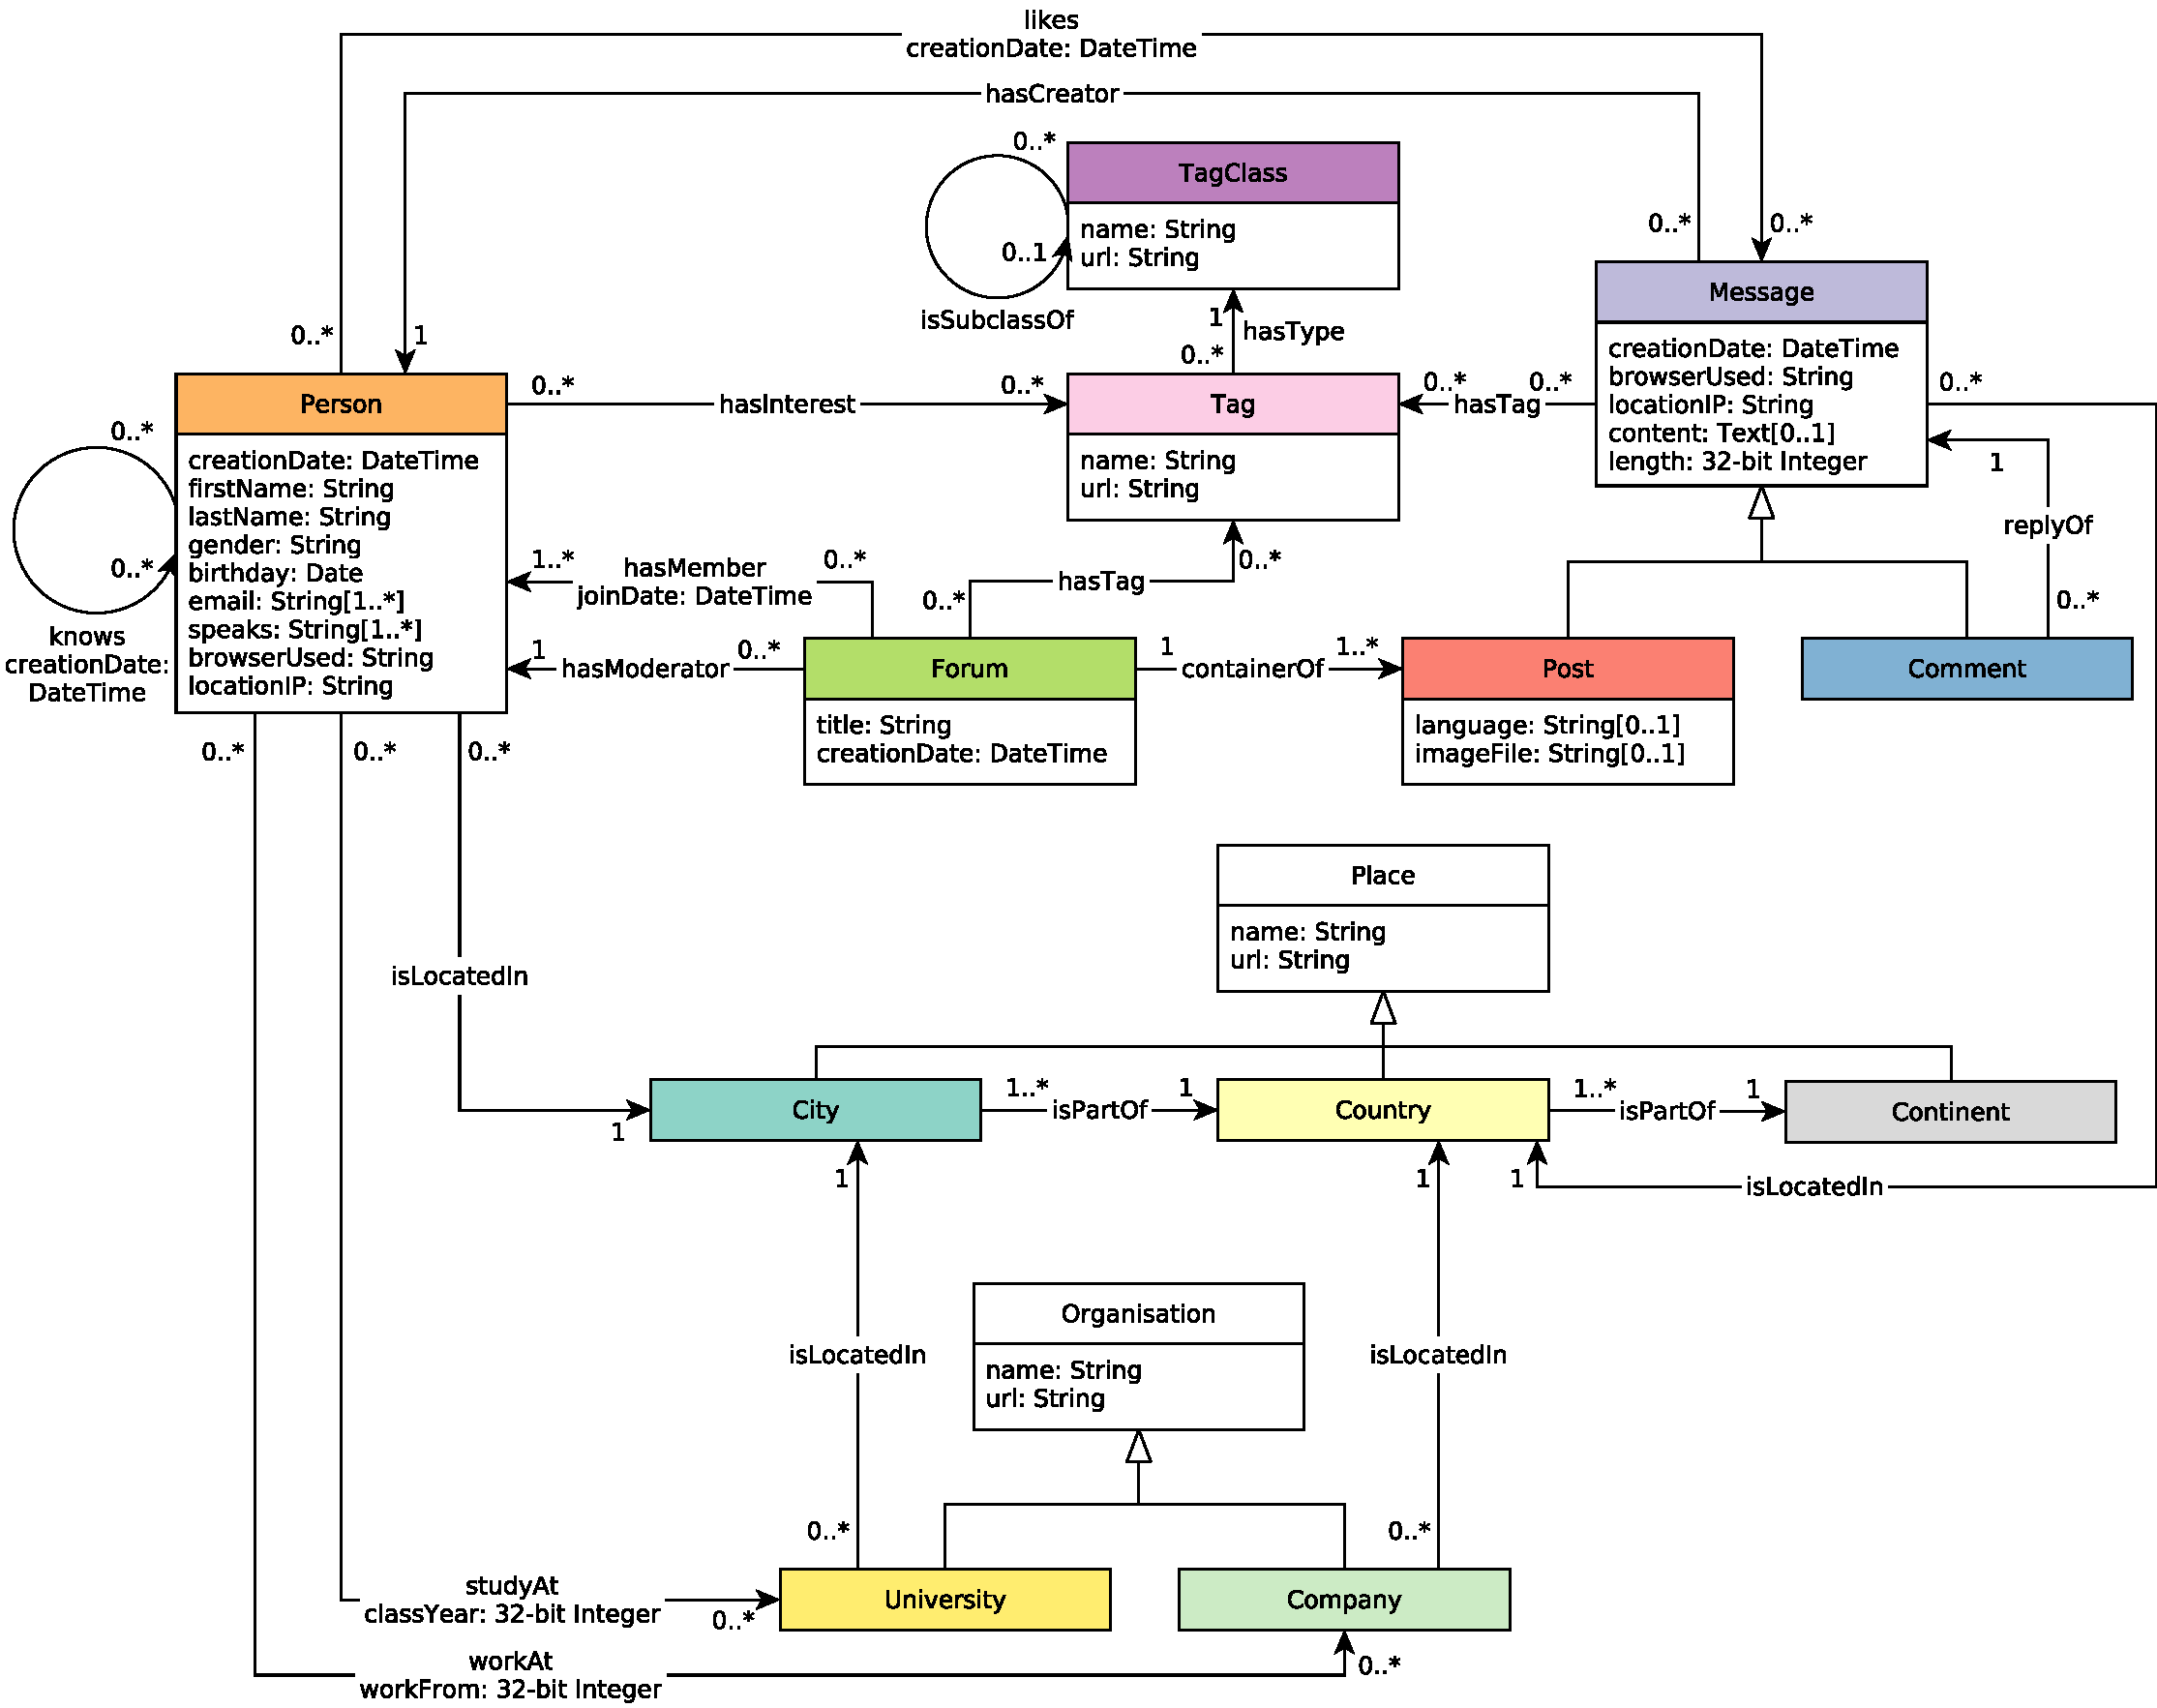
\includegraphics[width=\linewidth]{schema.pdf}
	\caption{Az LDBC Social Network Benchmark gráf sémája}
	\label{fig:dataschema}
\end{figure}

\section{Q1 lekérdezés differenciális adatfolyama}
\label{sec:q1-ddf}

\begin{figure}[h]
	\centering
	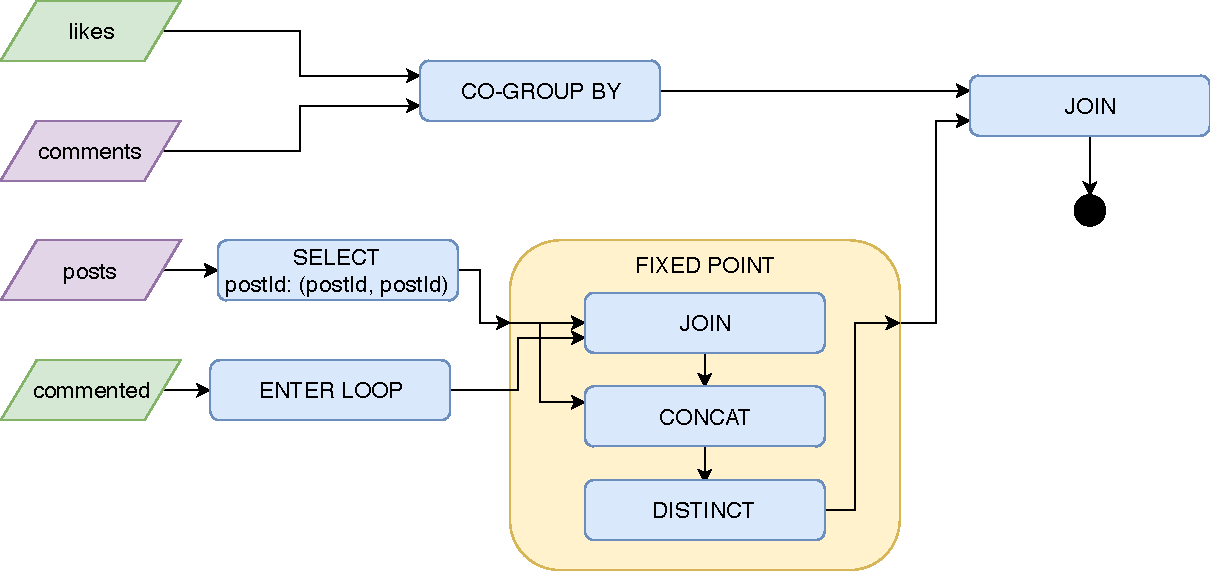
\includegraphics[width=\linewidth]{task1.pdf}
	\caption{A TTC Social Network feladat Q1 lekérdezésének differenciális adatfolyama}
	\label{fig:q1-ddffig}
\end{figure}

%\label{page:last}
\end{document}
